% This is a template for Ph.D. dissertations in the UCI format.
% 
% All fonts, including those for sub- and superscripts, must be 10
% points or larger.  Recommended sizes are 14-point for chapter
% headings, 12-point for the main body of text and figure/table
% titles, and 10-point for footnotes, sub- and super-scripts, and text
% in figures and tables.
%
% Notes: Add short title to figures, sections, via square brackets,
% e.g. \section[short]{long}.
%
\documentclass[12pt,fleqn]{ucithesis}
%\documentclass[12pt,fleqn]{report}

% 
% % A few common packages
% \usepackage{amsmath}
\usepackage{amsthm}
\usepackage{array}
\usepackage{relsize}
% 

\usepackage{tabularx}

% My Packages:
\usepackage{tikz}
\usepackage{natbib}
\usepackage{longtable}
\usepackage{multicol}
\usepackage{multirow}
\usepackage{paralist}
\usepackage{booktabs}
\usepackage[bf]{caption}
\usepackage{subcaption}  % \begin{subfigure}...\end{subfigure} within figure
\usepackage{soul}
\usepackage{graphicx}
\usepackage[normalem]{ulem}


\usepackage[nointegrals]{wasysym}





% other libraries that I use
\usepackage{amsmath,amssymb}
\usepackage{colortbl}
\usepackage{calc}
\usepackage{color}
\usepackage{fancybox}
%\usepackage{subfigure}
\usepackage{verbatim}
\DeclareGraphicsRule{.tif}{png}{.png}{`convert #1 `dirname #1`/`basename #1 .tif`.png}
\usepackage{float,wrapfig}
\usepackage{ifthen}


% \usepackage{lmodern}
% \usepackage[T1]{fontenc}

% \usepackage{fouriernc}
% \usepackage[T1]{fontenc}

\usepackage{tgschola}
\usepackage[T1]{fontenc}

% \usepackage[defaultsans]{droidsans}
% \usepackage{concmath}
% \usepackage[T1]{fontenc}

% \usepackage{droid}
% \usepackage[T1]{fontenc}

% \renewcommand*\familydefault{\sfdefault} %% Only if the base font of the document is to be typewriter style
% \usepackage[T1]{fontenc}
% 
% \usepackage[lf]{electrum}


% \usepackage{kpfonts}
% \usepackage[T1]{fontenc}

% \usepackage{kpfonts} %%
% \renewcommand*\familydefault{\sfdefault} %% Only if the base font of the document is to be sans serif
% \usepackage[T1]{fontenc}

% \usepackage[default,osfigures,scale=0.95]{opensans} %% Alternatively
% %% use the option 'defaultsans' instead of 'default' to replace the
% %% sans serif font only.
% \usepackage[T1]{fontenc}

% \usepackage{nimbus}
% \renewcommand*\familydefault{\sfdefault} %% Only if the base font of the document is to be sans serif
% \usepackage[T1]{fontenc}


% \usepackage[defaultsans]{droidsans}
% \renewcommand*\familydefault{\sfdefault} %% Only if the base font of the document is to be sans serif
% \usepackage[T1]{fontenc}

% \usepackage{lmodern}
% \renewcommand*\familydefault{\sfdefault} %% Only if the base font of the document is to be sans serif
% \usepackage[T1]{fontenc}

% \usepackage{fourier}
%\usepackage{mathptmx}
% \usepackage{tgschola} % option
% \usepackage{bookman} % option
%\usepackage{gfsdidot}
%\usepackage{courier}
% \usepackage{bera}
%\usepackage{palatino}
%\usepackage{times}
%\usepackage[math]{anttor}
% \usepackage[garamond]{mathdesign}

% \usepackage[T1]{fontenc}
% % \usepackage{charter}
% \usepackage[utopia]{mathdesign}

%\usepackage[scaled]{beramono}



\usepackage{listings}
\usepackage{textcomp}
\usepackage{setspace}


\renewcommand{\lstlistlistingname}{List of Code}
\renewcommand{\lstlistingname}{Code Listing}

\definecolor{shade}{HTML}{D4D7FE}
\definecolor{gray}{gray}{0.5}
\definecolor{green}{rgb}{0,0.5,0}

\lstnewenvironment{python}[1][]{
\lstset{
language=python,
basicstyle=\ttfamily\small\setstretch{1},
stringstyle=\color{red},
tabsize=4,
showstringspaces=false,
alsoletter={1234567890},
otherkeywords={\ , \}, \{},
keywordstyle=\color{blue},
emph={access,and,break,class,continue,def,del,elif,else,%
except,exec,finally,for,from,global,if,import,in,is,%
lambda,not,or,pass,print,raise,return,try,while},
emphstyle=\color{black}\bfseries,
emph={[2]True, False, None, self},
emphstyle=[2]\color{green},
emph={[3]from, import, as},
emphstyle=[3]\color{blue},
upquote=true,
morecomment=[s]{"""}{"""},
breaklines=true,
commentstyle=\color{green}\slshape,
emph={[4]1, 2, 3, 4, 5, 6, 7, 8, 9, 0},
emphstyle=[4]\color{blue},
literate=*{:}{{\textcolor{blue}:}}{1}%
	{=}{{\textcolor{blue}=}}{1}%
	{-}{{\textcolor{blue}-}}{1}%
	{+}{{\textcolor{blue}+}}{1}%
	{*}{{\textcolor{blue}*}}{1}%
	{!}{{\textcolor{blue}!}}{1}%
	{(}{{\textcolor{blue}(}}{1}%
	{)}{{\textcolor{blue})}}{1}%
	{[}{{\textcolor{blue}[}}{1}%
	{]}{{\textcolor{blue}]}}{1}%
	{<}{{\textcolor{blue}<}}{1}%
	{>}{{\textcolor{blue}>}}{1}%
	{\_}{}{0\discretionary{\_}{}{\_}},%
framexleftmargin=1mm, framextopmargin=1mm, frame=shadowbox, rulesepcolor=\color{blue},#1
}}{}


\newfloat{floater}{thp}{floater}[chapter]
\floatname{floater}{Floater}




%%%%%%   END LOAD LIBRARIES   %%%%%%   


%%%%%%       Define Colors
\definecolor{grey}{RGB}{152,152,152}
\definecolor{brick}{RGB}{160,0,0}
% % % Math Definitions: 
\DeclareMathOperator*{\median}{median} 


% commands for common volumes and things that are annoying to type
\newcommand{\phic}{$\phi$C31}
\newcommand{\mul}{$\mu$l}
%\newcommand{\ul}{$\mu$l}
\newcommand{\ug}{$\mu$g}
\newcommand{\uM}{$\mu$M}
\newcommand{\degree}{\ensuremath{^\circ}}
\newcommand{\C}{\degree C}
\newcommand\water{H$_2$O}
\newcommand\chlf{CHCl$_3$}
\newcommand\chkBox{ {\Square} }
\newcommand\chkBoxX{ {\CheckedBox} }




% miniSolns are little on-the-spot mixes rather than stock solutions
% \newcommand\miniSoln[1]{%
%         %\bigskip
%         \begin{center}\sffamily%
%                 \ovalbox{\parbox[l]{5in}{\vskip1ex \hskip1ex \textbf{Solution:} \textcolor{black}{#1}}}%
%         \end{center}%
%         %\bigskip%
% }

\newcommand\synopsis[1]{%
        %\bigskip
        \begin{center}%
                \fbox{
					\begin{minipage}[c]{.95\linewidth}
					\vskip1ex \hskip1ex \textbf{Synopsis: \\} \textcolor{black}{#1}
					\end{minipage}
				}%
        \end{center}%
        %\bigskip%
}

\newcommand\topicBox[2]{%
        %\bigskip
        \begin{center}%
                \fbox{
					\begin{minipage}[c]{.95\linewidth}
					\vskip1ex \hskip1ex \textbf{#1 \\} \textcolor{black}{#2}
					\end{minipage}
				}%
        \end{center}%
        %\bigskip%
}

% bioCheats are hacks that might work as a last resort to fix a failed experiment
\newcommand\bioCheat[1]{%
        %\bigskip
        \begin{center}\sffamily% 
                \ovalbox{\parbox[l]{5in}{\textbf{Bio-cheats:} \textcolor{green}{#1}}}%
        \end{center}%
        %\bigskip%
}

% bioTip are little suggestions for getting slightly better results or optimization
\newcommand\bioTip[1]{%
        %\bigskip
        \begin{center}\sffamily%
                \ovalbox{\parbox[l]{5in}{\textbf{BioTip:} \textcolor{green}{#1}}}%
        \end{center}%
        %\bigskip%
}

% valuable lessons are little problems that you finally figure out how to solve
\newcommand\valuableLesson[1]{%
	%\bigskip
	\begin{center}\sffamily%
		\ovalbox{\parbox[l]{5in}{\textbf{Valuable Lesson:} \textcolor{blue}{#1}}}%
	\end{center}%
	%\bigskip%
}

% gotchas are things that could cause your experiment to fail if you aren't careful
\newcommand\gotcha[1]{%
	%\bigskip
	\begin{center}\sffamily%
		\ovalbox{\parbox[l]{5in}{\textbf{Gotchas:} \textcolor{red}{#1}}}%
	\end{center}%
	%\bigskip%
}

% this is how I link to raw data
% you have to update this url to whereever you put your own data

% brief conclusions sum up a section
\newcommand\briefConclude[1]{\paragraph{Brief Conclusions:} #1}

% brief updates are added later after I learn something that might be relevant to a previous section
%\newcommand\briefUpdate[2]{\paragraph{Brief Update \emph{#1}:} \textcolor{magenta}{#2}}
\newcommand\briefUpdate[2]{%
	%\bigskip
	\begin{center}%
	\begin{tikzpicture}
 		\node [fill=shade,rounded corners=7pt]
		{ \parbox[l]{6in}{\bsf{Brief Update \emph{#1}:} \textcolor{magenta}{\bsf{#2}}} };
	\end{tikzpicture}
	\end{center}%
	%\bigskip%
}

% to dos are temporary reminders of stuff I'd like to do;  I usually try to remove 
% them after I've done the stuff.
\newcommand\toDo[1]{\paragraph{\textcolor{green}{To Do!!!}}\textcolor{red}{#1}}

% format a file name
\newcommand\fName[1]{\texttt{\textcolor{green}{#1}}}

% format a simple command
\newcommand\cmd[1]{\texttt{\textcolor{brick}{#1}}}

% format a bold sans serif
\newcommand\bsf[1]{\textbf{\textsf{#1}}}

% format a sans serif
\newcommand\nsf[1]{\textsf{#1}}

% Alert text Style
\newcommand\alert[1]{\textcolor{magenta}{#1}}

% rArrow short
\newcommand\rArw{$\Rightarrow$}

% et al
\newcommand\etal{\textit{et al.}}

%paraBreak
\newcommand{\pb}{\vskip2.5ex}

\newcommand{\CITEME}{\alert{CITEME}}

% BLIND TEXT DEFINITIONS
\usepackage{lipsum}
\newcommand{\dummytext[1]}{\alert{\lipsum[#1]}}


% plainpages=false fixes the "duplicate ignored" error with page counters
% Set pdfborder to 0 0 0 to disable colored borders around PDF hyperlinks
\usepackage[plainpages=false,pdfborder={0 0 0},colorlinks]{hyperref}
% \usepackage[plainpages=false,pdfborder={0 0 0}]{hyperref}


\usepackage[acronym]{glossaries}
\makeglossaries


\newglossaryentry{hemolymph}{name=hemolymph,
description={A fluid analogous to blood that constitutes the circulatory system of most invertebrates}}

\newglossaryentry{gene-drive}{name={gene drive},
description={molecular genetic tactics that cause a linked trait or gene to spread through a population at faster rates than expected based on fitness alone; generally operating independently of natural selection and genetic drift}}
	
\newglossaryentry{transposon}{name=transposon,see=transposable-element}
\newglossaryentry{transposable-element}{name=transposable element,
description={relatively short regions of DNA in an organism's genome that have the ability to cut (or copy) themselves from the genome and insert themselves into a new location in the genome}}
	
\newglossaryentry{effector-gene}{name={effector gene},
description={a gene that will cause the desired change in the environment of the mosquito or other vector.  An example might be a gene that codes for a protein that targets and destroys the pathogen}}

\newglossaryentry{prevalence}{name=prevalence,
description={the number or proportion of cases or events or attributes among a given population}}

\newglossaryentry{incidence}{name=incidence,
description={a measure of the frequency with which new cases of illness, injury, or other health condition occurs among a population during a specified period}}

\newglossaryentry{midgut}{name=midgut,
description={the location in the mosquito's digestive system where the bloodmeal is processed}}

\newglossaryentry{vector}{name=vector,
description={an organism that facilitates the transfer of pathogens from one host to another}}


%\newacronym{<label>}{<abbrv>}{<full>}

\newacronym{TS}{TS}{Total Score}

\newacronym{HMM}{HMM}{hidden Markov model}

\newacronym{SGE}{SGE}{\gls{SunGridEngine}}

\newacronym{MOODS}{MOODS}{MOtif Occurrence Detection Suite}

\newacronym{Argot2}{Argot2}{Annotation Retrieval of Gene Ontology Terms (\url{http://www.medcomp.medicina.unipd.it/Argot2/})}

\newacronym{RNA-Seq}{RNA-Seq}{RNA sequencing}

\newacronym{DNA-Seq}{DNA-Seq}{DNA sequencing}

\newacronym{ChIP-Seq}{ChIP-Seq}{chromatin immunoprecipitation followed by DNA-Seq}

\newacronym{FDR}{FDR}{false discovery rate}

\newacronym{PyPI}{PyPI}{Python Package Index}

\newacronym{gFunc}{gFunc}{graph-based functional genomics framework}

\newacronym{STEME}{STEME}{Suffix Tree Em for Motif Elicitation}

\newacronym{MEME}{MEME}{Multiple Em for Motif Elicitation}

\newacronym{PTCI}{PTCI}{Phylogenetic Transcriptional Correlation Index}

\newacronym{mAP}{mAP}{mRNA accumulation profile}

\newacronym{20E}{20E}{20-hydroxyecdysone}

\newacronym{JH}{JH}{juvenile hormone}

\newacronym{EIP}{EIP}{extrinsic incubation period}

\newacronym{dpi}{dpi}{days post infection}

\newacronym{ROS}{ROS}{reactive oxygen species}

\newacronym{DENV}{DENV}{dengue virus}

\newacronym{DENVI}{DENVI}{dengue virus infected}

\newacronym{DENV2}{DENV2}{dengue virus serotype 2}

\newacronym{Rex-D}{Rex-D}{Rexville D Puerto Rico}

\newacronym{CTM}{CTM}{Chetumal}

\newacronym{LVP}{LVP}{Liverpool}

\newacronym{AMP}{AMP}{attacin}

\newacronym{NBF}{NBF}{non-bloodfed}

\newacronym{TSS}{TSS}{transcriptional start sites}

\newacronym{SCOPE}{SCOPE}{Suite for Computational identification Of Promoter Elements}

\newacronym{PBM}{PBM}{post bloodmeal}

\newacronym{RNAi}{RNAi}{RNA interference}

\newacronym{NFKB}{\nfkb}{Nuclear Factor $\kappa$-light-chain-enhancer of activated B cells}

\newacronym{MDOS}{MDOS}{Motif Discovery using Orthologous Sequences}

\newacronym{Mya}{Mya}{million years ago}

\newacronym{FPKM}{FPKM}{fragments per kilobase of transcript per million mapped reads}

\newacronym{CRE}{CRE}{\textit{cis}-regulatory element}

\newacronym{CRM}{CRM}{\textit{cis}-regulatory module}

\newacronym{RIDL}{RIDL}{release of insects carrying a dominant lethal phenotype}

\newacronym{SIT}{SIT}{sterile insect technique}

\newacronym{TF}{TF}{transcription factor}

\newacronym{TFBS}{TFBS}{transcription factor binding site}

% Uncomment the following two lines to use the algorithm package,
% which provides an algorithm environment similar to figure and table
% ("\begin{algorithm}...\end{algorithm}"). A list of algorithms will
% automatically be added in the preliminary pages. Note that you
% probably want a package for the actual code to go with this (e.g.,
% algorithmic).
%\usepackage{algorithm}
%\renewcommand{\listalgorithmname}{\protect\centering\protect\Large LIST OF ALGORITHMS}

% Uncomment the following line to enable Unicode support. This will allow you
% to enter non-ASCII characters (such as accented characters) directly without
% having to use LaTeX's awkward escape syntax (e.g., \'{e})
% NOTE: You may have to install the ucs.sty package for this to work. See:
% http://www.unruh.de/DniQ/latex/unicode/
\usepackage[utf8x]{inputenc}

% Uncomment the following to avoid "widowing", where page breaks cause
% single lines of paragraphs to float onto the next page (this is not
% a UCI requirement but more of an aesthetic choice).
\widowpenalty=10000
\clubpenalty=10000

% Modify or extend these at will.
\newtheorem{theorem}{{\sc Theorem}}[chapter]
\newtheorem{definition}{{\sc Definition}}[chapter]
\newtheorem{example}{{\sc Example}}[chapter]

% Uncomment the following to have numbered subsubsections (by default
% numbering goes only to subsections).
%\setcounter{secnumdepth}{4}


% Set this to only select a subset of the includes directives below.
% Very handy to speed up compilation if you're working on a certain
% part of your thesis. It conserves page numbers, references, etc.
% even for non-included files.
\includeonly{0_introduction,appendix}

\begin{document}

% Preliminary pages are always loaded (TOC, CV, etc.)
\thesistitle{
  Comparative transcriptomics of blood-feeding in midguts of three disease-vector mosquito species
}

\degreename{Doctor of Philosophy}

% Use the wording given in the official list of degrees awarded by UCI:
% http://www.rgs.uci.edu/grad/academic/degrees_offered.htm
\degreefield{Biological Sciences}

% Your name as it appears on official UCI records.
\authorname{William Augustine Dunn III}

% Use the full name of each committee member.
\committeechair{Anthony A. James}
\othercommitteemembers
{
  Xiaohui Xie\\
  Donald F. Senear
}

\degreeyear{2014}

\copyrightdeclaration
{
\todo[inline]{add copy-write text to preliminaries}
  {\copyright} {\Degreeyear} \Authorname
}

% If you have previously published parts of your manuscript, you must list the
% copyright holders; see Section 3.2 of the UCI Thesis and Dissertation Manual.
% Otherwise, this section may be omitted.
% \prepublishedcopyrightdeclaration
% {
% 	Chapter 4 {\copyright} 2003 Springer-Verlag \\
% 	Portion of Chapter 5 {\copyright} 1999 John Wiley \& Sons, Inc. \\
% 	All other materials {\copyright} {\Degreeyear} \Authorname
% }

% The dedication page is optional.
\dedications
{

For my unbelievably smart, funny, beautiful, and immeasurably supportive wife, Sarah.
The last year would not have been remotely possible without the mental and material support that she so generously provides in spades. 

For my parents.
Thank you for encouraging and \textit{indulging} the interests and behaviors of a young boy flirting with the natural world and how things are put together.
Thank you for providing grandparent-quality childcare to Liam for so long while I worked on this document.
Neither would I have been able to achieve this without you both.

For my son Liam, you are an inspiration of raw, unbridled energy and joy.
A true force to behold!
}

\acknowledgments
{
% 

I would like to thank those entities whose funding made this work possible.
% NLM/NIH
% PSWRCE

In addition, the inclusion of our previous articles discussed in this document was made possible by the generous policies of --PUBLISHERS--.

Professor Xiaohui Xie and his students provided much appreciated advice and tutorship in the computational realm.
Professor Donald Senear provided insightful commentary as well as his valuable time during committee meetings and private consultation.
Finally, I must thank Professor Anthony James for his invaluable advice and mentorship as well as his moral support.

%   
%   (You must acknowledge grants and other funding assistance. 
%   
%   You may also acknowledge the contributions of professors and
%   friends.
%   
%   You also need to acknowledge any publishers of your previous
%   work who have given you permission to incorporate that work
%   into your dissertation. See Section 3.2 of the UCI Thesis and
%   Dissertation Manual.)
}


% % Some custom commands for your list of publications and software.
% \newcommand{\mypubentry}[3]{
%   \begin{tabular*}{1\textwidth}{@{\extracolsep{\fill}}p{4.5in}r}
%     \textbf{#1} & \textbf{#2} \\ 
%     \multicolumn{2}{@{\extracolsep{\fill}}p{.95\textwidth}}{#3}\vspace{6pt} \\
%   \end{tabular*}
% }
% \newcommand{\mysoftentry}[3]{
%   \begin{tabular*}{1\textwidth}{@{\extracolsep{\fill}}lr}
%     \textbf{#1} & \url{#2} \\
%     \multicolumn{2}{@{\extracolsep{\fill}}p{.95\textwidth}}
%     {\emph{#3}}\vspace{-6pt} \\
%   \end{tabular*}
% }

% Include, at minimum, a listing of your degrees and educational
% achievements with dates and the school where the degrees were
% earned. This should include the degree currently being
% attained. Other than that it's mostly up to you what to include here
% and how to format it, below is just an example.
\curriculumvitae
{
\includepdf[pages=-]{CV/cv.pdf}
}
% {
% \todo[inline]{in-line my CV document and match styles}
% \textbf{EDUCATION}
%   
%   \begin{tabular*}{1\textwidth}{@{\extracolsep{\fill}}lr}
%     \textbf{Doctor of Philosophy in Computer Science} & \textbf{2012} \\
%     \vspace{6pt}
%     University name & \emph{City, State} \\
%     \textbf{Bachelor of Science in Computational Sciences} & \textbf{2007} \\
%     \vspace{6pt}
%     Another university name & \emph{City, State} \\
%   \end{tabular*}
% 
% \vspace{12pt}
% \textbf{RESEARCH EXPERIENCE}
% 
%   \begin{tabular*}{1\textwidth}{@{\extracolsep{\fill}}lr}
%     \textbf{Graduate Research Assistant} & \textbf{2007--2012} \\
%     \vspace{6pt}
%     University of California, Irvine & \emph{Irvine, California} \\
%   \end{tabular*}
% 
% \vspace{12pt}
% \textbf{TEACHING EXPERIENCE}
% 
%   \begin{tabular*}{1\textwidth}{@{\extracolsep{\fill}}lr}
%     \textbf{Teaching Assistant} & \textbf{2009--2010} \\
%     \vspace{6pt}
%     University name & \emph{City, State} \\
%   \end{tabular*}
% 
% \pagebreak
% 
% \textbf{REFEREED JOURNAL PUBLICATIONS}
% 
%   \mypubentry{Ground-breaking article}{2012}{Journal name}
% 
% \vspace{12pt}
% \textbf{REFEREED CONFERENCE PUBLICATIONS}
% 
%   \mypubentry{Awesome paper}{Jun 2011}{Conference name}
%   \mypubentry{Another awesome paper}{Aug 2012}{Conference name}
% 
% \vspace{12pt}
% \textbf{SOFTWARE}
% 
%   \mysoftentry{Magical tool}{http://your.url.here/}
%   {C++ algorithm that solves TSP in polynomial time.}
% 
% }

% The abstract should not be over 350 words, although that's
% supposedly somewhat of a soft constraint.
\thesisabstract
{
With the goal of executing a multi-dimentional comparative study of the transcriptomics of blood-feeding in midguts of \Aea, \Ang, and \Cxq, I have designed multiple software solutions to integrate and analyze \gls{RNA-Seq} data (midgut-specific time-course: 0, 4, 6, 8, 10h \gls{PBM}); orthology relationships; predicted \gls{20E} responsive transcription factor binding site locations, and promoter sequence conservation.
Using these tools, I compile gene sets that are simultaneously correlated by way of functionality (e.g. putatively \gls{20E}-regulated), evolutionary history, and maintenance of mRNA abundance-patterns across species-divergence times as large as 150 million years.  

Frequently, \gls{functional-genomics} approaches contain problems or subproblems that require generating biologically meaningful gene-sets.
Optimizing signal-to-noise ratios in data is a major challenge to generating useful gene-sets.
The rise of the Omics Era presents the challenge of integrating data from multiple large-scale input streams in an informative way.
Network Graphs offer a natural framework for storing and analyzing highly dimensional relationships and have provided insight when applied to areas such as gene interaction relationships as well as human relationships.

This project leverages 3-way 1:1 orthology relationships to successfully target \glspl{mAP} associated with the \gls{20E} regulatory program in the midguts of the three divergent mosquito species for functional annotation and review.
}


%%% Local Variables: ***
%%% mode: latex ***
%%% TeX-master: "thesis.tex" ***
%%% End: ***

\preliminarypages

% Include the different components of your thesis, in separate files.
% Using \include allows you to set \includeonly above.
\chapter{Introduction}

\section{Purpose}

Introduce core concepts relating to my project such as:

\begin{enumerate}
\item Importance of Dengue and Malaria
\item Transmission cycle dependent on Mosquitoes
\item Limited effectiveness (medical/finacial) of treatment of the diseases in rural poor human communities
\item Vector Control Strategies
\item How Transgenesis modifies the vector control landscape
\item Elements of Successful Transgenesic Vector Control
\item Introduction to control of transcription and imoprtance of \glspl{CRE}/\glspl{CRM}
\end{enumerate}


\section{Dengue fever and malaria are mosquito borne diseases}

\synopsis{
\begin{itemize}
\item there are many but we focus on Dengue Fever and Malaria
\item causative agents are RNA viruses and Plasmodium protists, respectively
\item people don't give people these two diseases
\item mosquitoes generally don't give mosquitoes these diseases
\end{itemize}
}

There are many mosquito borne diseases that afflict the world's population; \alert{however, the James Lab focuses on two of the major ones: dengue fever and malaria}.
The causative agents of these two diseases are a suite of four species of RNA viruses (Dengue Virus 1-4) and a suite of five species of protist from the genus \textit{Plasmodium}, respectively.
However, in any \textbf{single} geographic location they are generally transmitted by a single species of mosquito \alert{CITEME}. 

\alert{TABLE HERE}

The fact that both of these diseases are caused by multiple pathogen species complicates efforts to prevent human disease: particularly when addressed from the perspective of providing therapeutic or prophylactic care directly to human patients.

\section{The transmission cycles of dengue fever and malaria require mosquitoes}

Another very important aspect of both of these diseases is that people do not become infected through interaction with other people, and mosquitoes do not become infected through interaction with other mosquitoes.
The transmission cycles transmission of both diseases require that the pathogen be passed from human to mosquito or from mosquito to human.
This pattern has important consequences that we can exploit to prevent the transmission cycle from producing as many infected individuals.

\subsection{Transmission cycle}

\begin{enumerate}
\item a female mosquito bites infected person
\item the pathogen is taken into mosquito midgut with bloodmeal
\item the pathogen must escape the midgut and gain access to the mosquito's circulatory system (the animal is now \textbf{infected})
\item the pathogen must gain access to the mosquito's salivary glands (the animal is now \textbf{infectious})
\item the infectious female mosquito bites an uninfected human and pathogens in her saliva are introduced to the person's body
\end{enumerate}
While the specifics of how viruses and protists live and reproduce in mosquitoes and humans are quite different, the transmission cycles of dengue and malaria are very similar in their major events.
The transmission of either pathogen from one infected human to another can both be summarized into five fundamental events.
First, a female mosquito feeds on an infected human's blood taking up the pathogen as well.
The bloodmeal is digested in the mosquito's midgut, \alert{and as you might expect, the midgut is the first stop for the pathogen too.}
Escape of the midgut is the first critical step for the survival of the pathogen inside the mosquito.
If it is trapped in the midgut, it will eventually be passed as waste after the bloodmeal is digested.
If it manages to escape to the \gls{hemolymph}, the pathogen must gain access to the mosquito's salivary glands if it is to infect another human.
If this step is unsuccessful, then the mosquito, while itself \textbf{infected}, is not \textbf{infectious} to other humans.
For this, the pathogen must be injected into the bloodstream of the next human along with the contents of the mosquito's saliva.

\section{Public health: \emph{multiple targets}}

\synopsis{
\begin{itemize}
\item The specifics of the transmission cycle of these diseases provides multiple targets for public health interventions
\item focus on the human
\item focus on the vector
\end{itemize}
}

Because the arrow of transmission always\footnote{While some mosquito
  to non-human vertebrate transmission may occur, it is not thought to
  be sufficient to maintain the pathogen if the mosquito:human loop is
  broken.} points from mosquito to human or from human to mosquito, if either of those arrows are broken, the cycle will collapse and the area would eventually be cleared of the pathogen provided the intervention is maintained.
This model suggests that there are two primary targets for public health interventions aiming to reduce the \gls{incidence}
(followed by \gls{prevalence}) of infection in a population.

\begin{enumerate}
\item
  prevent mosquitoes from infecting humans
\item
  prevent humans from infecting mosquitoes
\end{enumerate}

However, many of the interventions can not be clearly divided into addressing purely the human or vector side of the cycle.
For example, any efforts to reduce the number of bites that humans receive from mosquitoes affects both the probabilities of the vector \emph{and} the human becoming infected.
This is one reason that vector control rather than purely human-based interventions are almost always part of prevention strategies.
For the purposes of this document, I will define human-based interventions to be those that are directly administered to the human's body.
Essentially: medical interventions.

It should be noted that in this respect, the long term goals of public health are more focused on prevention than the treatment of acute cases.

Of course sick people need to be treated, and finding and clearing people who are infected is a part of preventing mosquitoes from acquiring the pathogen from people.
However, in the long game it is much more effective to prevent the infection.
These efforts are what we will focus on.

\subsection{Options for the humans}

Because of the definition of human-based interventions that I am using, there are relatively few effective options in this category for malaria and dengue fever.
Normally, this section would include vaccines and swift, effective patient identification and treatment to clear the infection.
\alert{For reasons that will be discussed in a later post, these interventions simply do not exist on the market or in a cost-effective form applicable to the isolated and impoverished areas that are most affected.}

\subsection{Conventional options for the vectors}

Because medical options are generally quite scarce, most attention in the field is directed toward controlling access of the vector populations to human contact.
This can include removal of nearby mosquito breeding sites (usually standing water), spraying of insecticides, introduction of biological predators, and/or bed nets, etc.
One fairly novel approach that has implications for the next post in this series is sterile insect technique.



\subsection{Sterile Insect Technique}
\href{http://en.wikipedia.org/wiki/Sterile\_insect\_technique}{Sterile insect technique (SIT)} exploits a peculiar aspect of some insects' reproductive behavior. 
In many insects, it is only (or at least
primarily) the first mating event that ``matters''.
Subsequent mating events contribute little to no genetic material to the females progeny, \textbf{even when the first event involves a sterile male}.
This means that if massive numbers of sterilized males are introduced into a native population, any wild female that mates first with one of the sterile males will be effectively sterilized herself.
This can have dramatic effects on the local population.
For a famously effective SIT campaign, look up \href{http://goo.gl/DF7bv}{screwworm eradication} on google.


\section{Transgenic options for the vectors}

Most conventional vector control strategies involve what might be termed \textbf{vector population reduction}.
As we get into what transgenics can do for vector control, we will see that in addition to population reduction we have a new strategy available which has quite exciting implications to the sustainability of the vector control aspect of public health interventions for dengue and malaria.
This could be called \textbf{vector population conversion}.

\section{Introducing Inheritable Transgenes into the Mosquito Genome}

Before one can employ transgenic methods for vector control, one must of course have the ability to make transgenic vectors.
For mosquitoes, this is quite a bit more labor intensive than for other fly species like \emph{Drosophila melanogaster}.
However, it has been accomplished, and protocols to reliably introduce transgenes into many mosquito species now exist.
Unfortunately, the relative difficulty is still high, and it takes roughly 2-3 months before a stable line is established.
So while this step can be filed under ``accomplished'', work is constantly being done to improve its ease and efficiency.

The method of gene insertion into the genome generally relies on re-purposing the activities of small, ``parasitic'', mobile DNA elements called \glspl{transposon} or \glspl{transposable-element}.
These elements have the ability to cut themselves out of one part of the DNA and re-insert themselves into another.
We can engineer them in the lab to carry our genes instead of the genes that they usually contain.
This allows our genes to be inserted into the genome instead of the contents of the original transposon.

Until recently, most if not all transposons used inserted the genes into more-or-less random regions, and in single, double or \textbf{multiple} copies and/or locations \cite{Adelman2004}, \cite{Sethuraman2007}.
This makes characterizing the effects of the effector genes complicated.
However, with the successful implementation of the \href{http://en.wikipedia.org/wiki/Site-specific\_recombinase\_technology\#PhiC31\_Integrase}{phic31 site specific integration system} in \emph{Aedes aegypti} and \emph{Anopheles stephensi} \cite{Thorpe1998}, \cite{Nimmo2006}, \cite{Isaacs2012}, we can now reliably target specific, known regions of the genome for transgene integration of a single copy.

The ``heritable'' part is achieved through which cells take up the transgene.
Only certain types of cells have the ability to project their genetic code into the next generation.
In order to have a transgene be heritable by the following generations we must make sure that at least egg cells).

A peculiarity about fly development is that as the embryo is developing the cells that will become the germ line always position themselves at one end (or pole) of the embryo.
They earned the moniker ``pole cells''.
This makes targeting these cells for the transgene feasible.
When the solution containing the transgene construct is injected into the embryos, it is done where the pole cells are.
This means that the first set of mosquitoes that might be fully transgenic is not the set that you injected but the first generation of offspring that your injected mosquitoes produce.

\section{Effector Genes}

With the ability to integrate transgene constructs into the vectors' genomes, we need constructs that carry genes that will effect the response that we desire in the vector.
Two broad strategies are commonly applied when designing an anti-transmission phenotype.

\subsection{Vector Population Reduction:}

The goal of vector population reduction is the same as the conventional vector control modalities.
\emph{Reduce the size of the vector population to decrease the probability of infectious interactions between vectors and humans.}

\textbf{Conventional tactics} include removal of breeding sites through draining of swamps, removal of items that store water (tires, buckets, etc) where larvae develop from populated areas, and of course, chemical insecticidal campaigns.
Another, more recent tactic is sterile insect technique.

A \textbf{transgenic tactic} for the population reduction strategy is illustrated by \href{http://www.oxitec.com/}{Oxitec's} \emph{Aedes aegypti} strain \href{http://www.oxitec.com/health/our-products/aedes-agypti-ox3604c/}{OX3604C} developed with support from the \href{http://www.grandchallenges.org/Pages/Default.aspx}{Bill and Melinda Gates Foundation's Grand Challenges for Global Health Initiative}.
OX3604C, represents a female-specific \gls{RIDL} approach which uses a poison transgene that kills any female adult expressing the transgene unless the female is being fed the ``antidote'' through its water supply.

Releasing enough of these mosquitoes will affect the local mosquito species population in a way that is analogous to \gls{SIT}.

\subsection{Vector Population Replacement (Conversion):}

Vector population conversion is a novel strategy for vector control that only exists within the context of genetically altering the vectors.
This strategy actually promises to be the most long-lasting vector-focused intervention; because unlike \textbf{all} vector population reduction tactics, there is a theoretical point in a conversion intervention (the anti-transmission trait works and is present in local populations at near 100\%) when the human interaction can be ceased but the intervention continues to function.
For population reduction to approach this result, the vector species must not simply be eliminated from the local area, but approach elimination on a continental scale, or more realistically achieve global eradication.

The reason is that these mosquitoes (especially \emph{Aedes aegypti}) can and do travel long distances, as eggs or larvae, in the backs of trucks (between villages) or in the pools of water collected in super-tankers (transcontinentally).
So a local village is only free of the vectors until more migrate into the area.
But in a conversion scenario, those migrants mate with the local vector population, and their offspring are assimilated into transmission-deficient mosquitoes.
The protection of the local village can be preserved \emph{even if some surrounding villages fail to maintain control of their mosquitoes}.

An example of a \textbf{transgenic tactic} for population conversion of \emph{Aedes aegypti} into a transmission-deficient phenotype involves an effector gene that codes for double stranded portion of the target dengue virus as RNA \cite{Franz2006}, \cite{Mathur2010}.
Because most animal cells have a system that detects and degrades double stranded RNA
\footnote{Double stranded RNA generally signals that a virus is active in the cell.}
in a sequence specific manner, this primes the mosquito cells' antiviral response to specifically attack the dengue virus if the effector gene is expressed in the cell before it gets infected.

\section{Controlling When and Where the Effector Genes are Expressed}

Even armed with an effector gene that clears 100\% of the pathogen 100\% of the time, you will not be successful in limiting transmission if it is not turned on in the right time and place.
If your effector gene works best when the pathogen is in the midgut, but your gene is only expressed in the antennae, you have wasted your time.

The region of DNA directly before the sequence of the gene is \emph{usually} the most influential determinant of the pattern of expression and is referred to as the promoter.
It determines when the gene will be turned on (let's say directly following the ingestion of a bloodmeal), and in which tissue type (let's say the midgut).
The way that this is accomplished is due to the binding of special proteins called transcription factors that recognize specific DNA sequences.
Once bound to the promoter they recruit the special machinery needed for the gene to be turned on.

If we wanted to control a transgene in a specific way (turned on after a bloodmeal in the midgut), one way to go about it would be to identify genes in the mosquito that already have a similar expression pattern to the ideal that you want.
Then we could copy the promoter from that gene and paste it in front of our transgene
\footnote{The story is \textbf{of course} more complicated than this, and the replication of the
    original expression pattern may not always be perfect with this simplified method; however,
    it is suitably explanatory for our purposes at the moment.}.
Because we will have replicated the specific \glspl{TFBS} that control the original gene, our transgene should inherit a very similar expression pattern.

This is a very common process used to engineer the expression patterns of real transgenes in mosquitoes.
In \cite{Moreira2000}, the promoter sequences of a gene called carboxypeptidase (normally expressed in the midgut after a meal to help digest it) from \emph{Aedes aegypti} and \emph{Anopheles gambiae} were pasted in front of a transgene that causes the cells that express the gene to light up.
This type of transgene is called a \gls{reporter gene} because it allows the researchers to visualize the activity of the promoter used to drive its expression.

From the abstract of \cite{Moreira2000}:

\begin{quote}
Six independent transgenic lines were obtained with the AeCP construct and one with the
AgCP
construct.
Luciferase mRNA and protein were abundantly expressed in the
guts of transgenic mosquitoes in four of the six AeCP lines and in the
AgCP line.
Expression of the reporter gene was gut-specific and reached
peak levels at about 24 h post-blood ingestion.
\end{quote}

\section{Achieving Swift, Dramatic, and Clinically Meaningful Effects on the Native Vector Population}

In many ways, this is the most difficult part of the puzzle.
In order for the transgene to have its self-sustaining properties as well as achieve effective anti-transmission results, it must spread through the native mosquito population to the point that the percent of individuals possessing the gene approaches 100\%.

Optimistically assuming that the transgene carries a negligible fitness cost
\footnote{By fitness cost/advantage here, I mean that the transgene
    causes the mosquitoes that inherit it to be either less or more
    successful at producing offspring, respectively.},
or even a slight fitness advantage, achieving near 100\% conversion could take decades.
Funding terms for efforts like this in poor nations can be closer to 5 years or less.
To enable the population conversion strategies to work, we must come up with genetic ``tricks'' that cause the gene to spread through a mosquito population \textbf{much} faster than could happen naturally.
Efforts to discover or design this \gls{gene-drive} system are an on going and active area in this field.
\chapter{Development of Analytical Approach}

\section{Purpose}
Review a selection of my contributions to the literature that have informed the approach used in this project throughout my tenure as a member of the lab
\begin{enumerate}
 \item Comparative genomics allows the discovery of cis-regulatory elements in mosquitoes
  \begin{itemize}
   \item Use of comparative genomics to discover putative CREs from orthologous promoter regions in mosquitoes that were able to be corelated with bloodmeal associated transcription control
  \end{itemize}
 \item RNA-seq analyses of blood-induced changes in gene expression in the mosquito vector species, Aedes aegypti
  \begin{itemize}
   \item relevance
  \end{itemize}

 \item Strain Variation in the Transcriptome of the Dengue Fever Vector, Aedes aegypti
   \begin{itemize}
   \item relevance
  \end{itemize}
 \item Comparative Transcriptome Analyses of Deltamethrin-Resistant and-Susceptible Anopheles gambiae Mosquitoes from Kenya by RNA-Seq
   \begin{itemize}
   \item relevance
  \end{itemize}
 \item Complex Modulation of the Aedes aegypti Transcriptome in Response to Dengue Virus Infection
   \begin{itemize}
   \item relevance
  \end{itemize}
\end{enumerate}

\section{Comparative genomics allows the discovery of cis-regulatory elements in mosquitoes}


Figure \ref{fig:mosqPhyloTree}


Figure \ref{fig:sieglaff2009_full}



\begin{figure}[hp]

\hfil
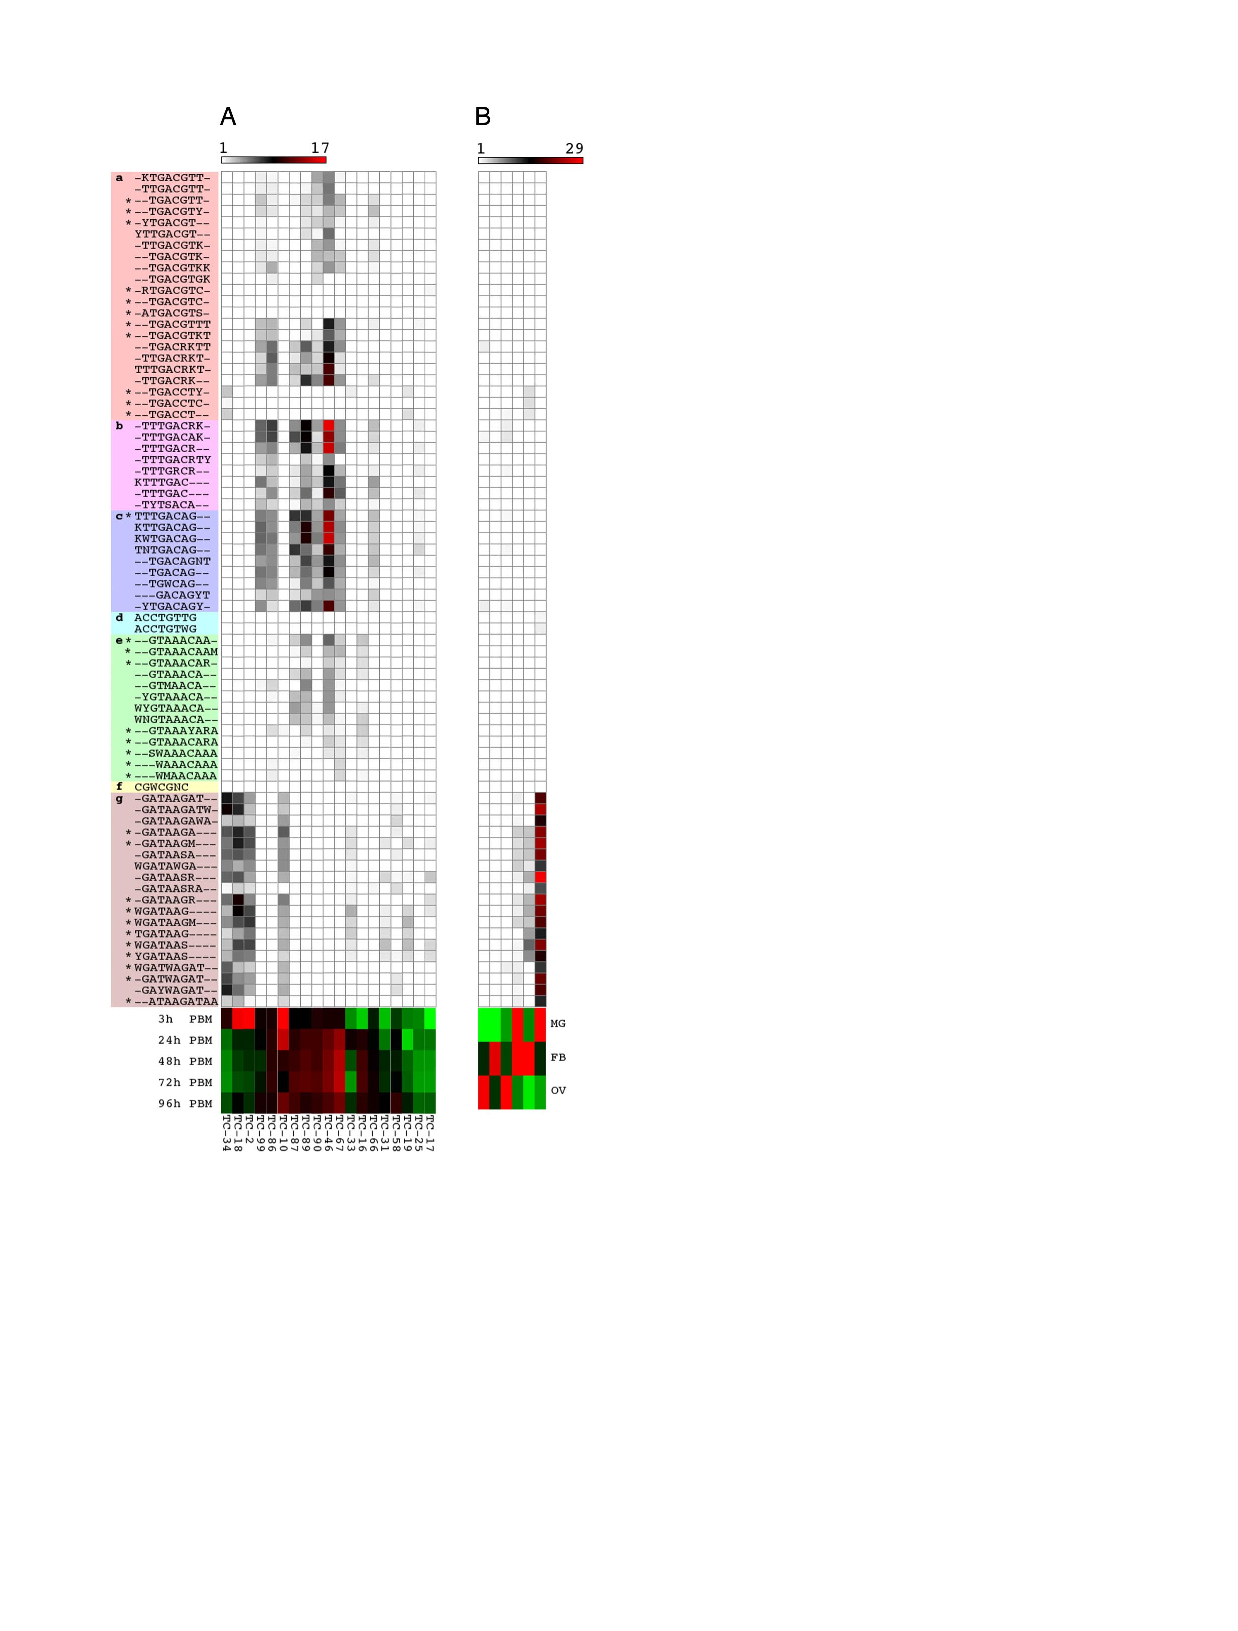
\includegraphics[scale=.95]{figures/figs/sieglaff2009_full.pdf}
\hfil
\caption[Associations of mosquito motifs with gene expression profiles in \Ag]{\bsf{Associations of mosquito motifs with gene expression profiles in \Ag:} \\ \sf
Motif enrichment within (A) 5′-end flanking regions of genes in clusters responsive to blood meal ingestion, and in (B) 5′-end flanking regions of genes in clusters enriched in selected tissues. The significance of motif enrichment is indicated by pseudocolor of -log10 (P-value) determined through hypergeometric statistics, and the median expression profile of each gene cluster is shown below each respective column. Red and green colors represent higher and lower relative mRNA accumulation, respectively. Asterisks (*) indicate a match to a previously described mosquito TFBS. Heatmaps were created with Matrix2png (\CITEME:local-58). FB, fat body; hPBM, hours post blood meal; MG, midgut; OV, ovaries; TC, time course clusters.

Adapted from \cite{Sieglaff2009}}
\label{fig:sieglaff2009_full}
\end{figure}

\begin{figure}[hp]
\centering

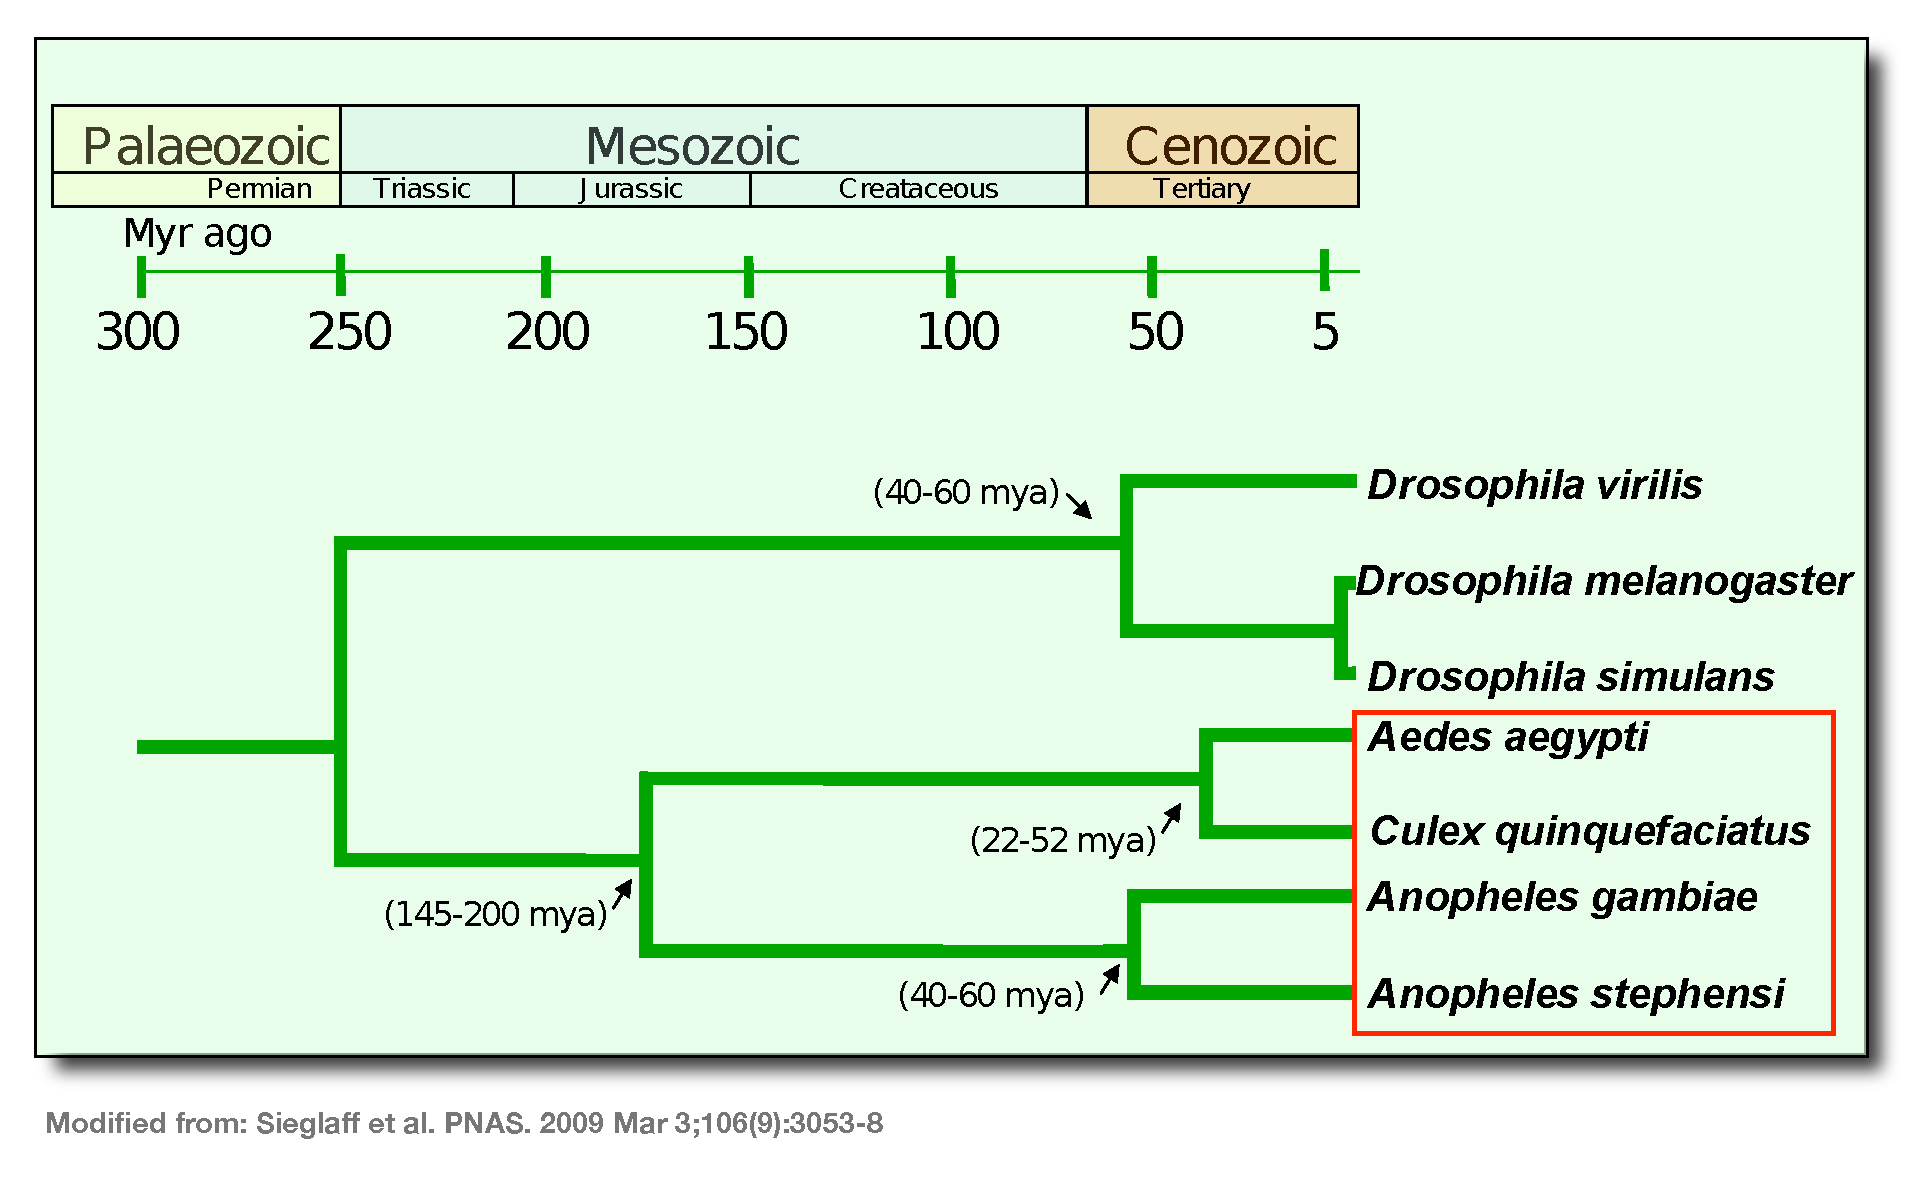
\includegraphics[width=.7\textwidth]{figures/figs/mosqPhyloTree.pdf}

\caption[Phylogenetic relationships between four vector mosquitoes]{\bsf{Phylogenetic relationships between four vector mosquitoes compared with representative \textit{Drosophila} species:} \\ \sf
\dummytext[1]

Adapted from \cite{Sieglaff2009}}
\label{fig:mosqPhyloTree}
\end{figure}


\section{RNA-seq analyses of blood-induced changes in gene expression in the mosquito vector species, Aedes aegypti}

Figure \ref{fig:aedesHMMsplice}


Figure \ref{fig:bonnizoniCREs}


\begin{figure}[hp]
\centering
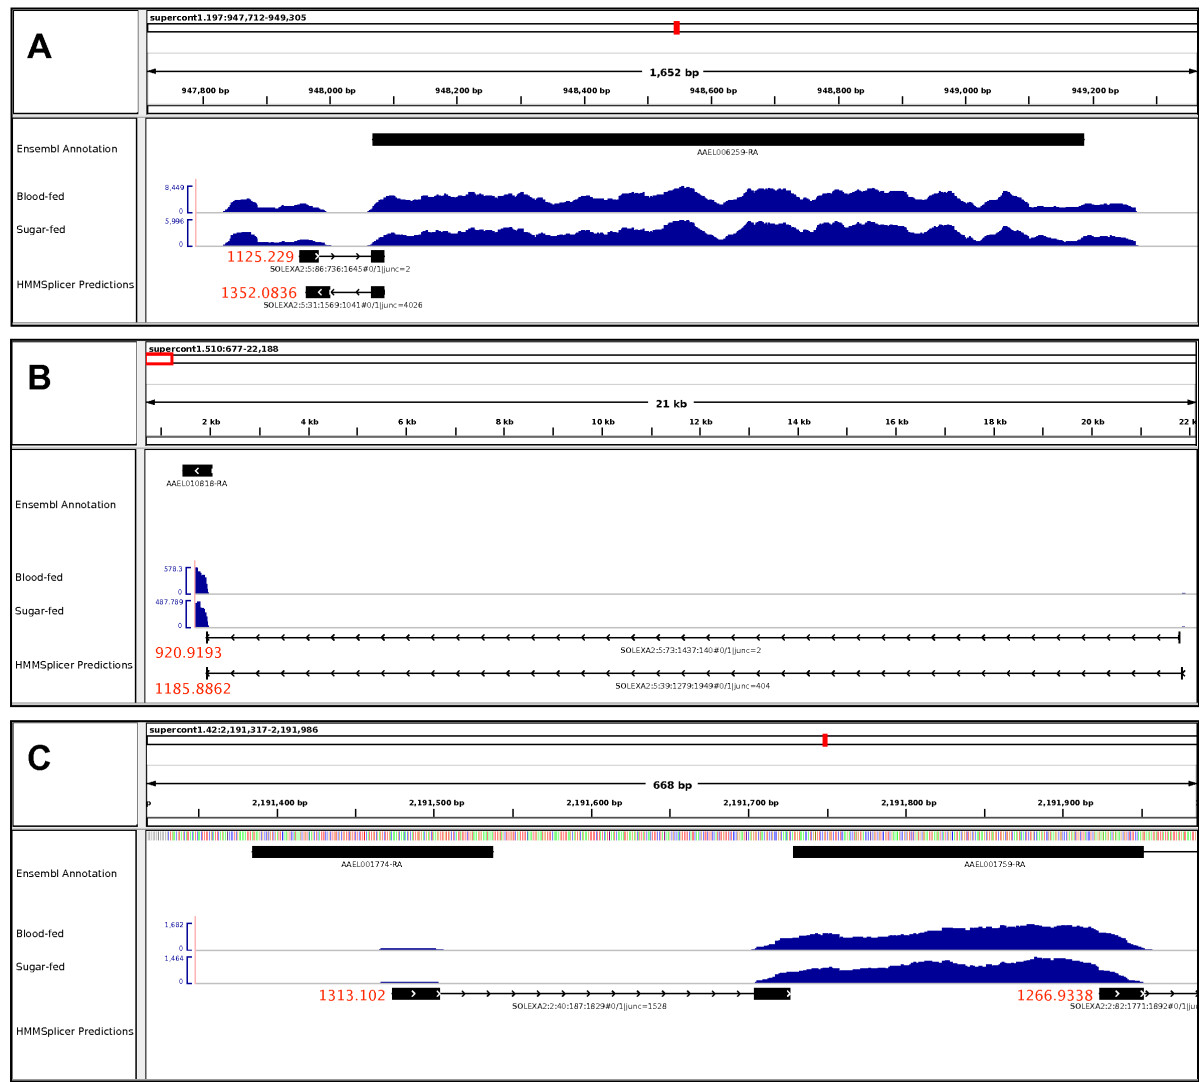
\includegraphics[width=.95\textwidth]{figures/figs/aedesHMMsplice.jpg}

\caption[Examples of amendments to the \Aa\ annotation supported by HMMSplicer results]{\sf \textbf{Examples of amendments to the \Aa\ annotation supported by HMMSplicer results:} Black bars in the top tracks represent the current gene annotations. Blue histograms in the second track represent the non-normalized coverage of RNA-seq reads at each position. The range of the histogram values shown in each view is depicted on the labeled y-axis of each RNA-seq track. Black boxes in the lower track represent splice-site predictions based on the RNA-seq reads using HMMSplicer determined in this study. Each function has a unique identifier listed below and its HMMSplicer score is listed in red. If multiple reads support a single junction, "junc = x" lists the number of supporting reads. This information provides evidence to link two islands of transcription as a single transcription event, therefore, exons of a common mRNA. All predicted junctions shown here also are supported by EST alignments. Genes are (A) AAEL006259; (B) AAEL010818; and (C) AAEL001774 and AAEL001759.

Excerpted from \cite{Bonizzoni2011}}
\label{fig:aedesHMMsplice}
\end{figure}

\begin{figure}[hp]

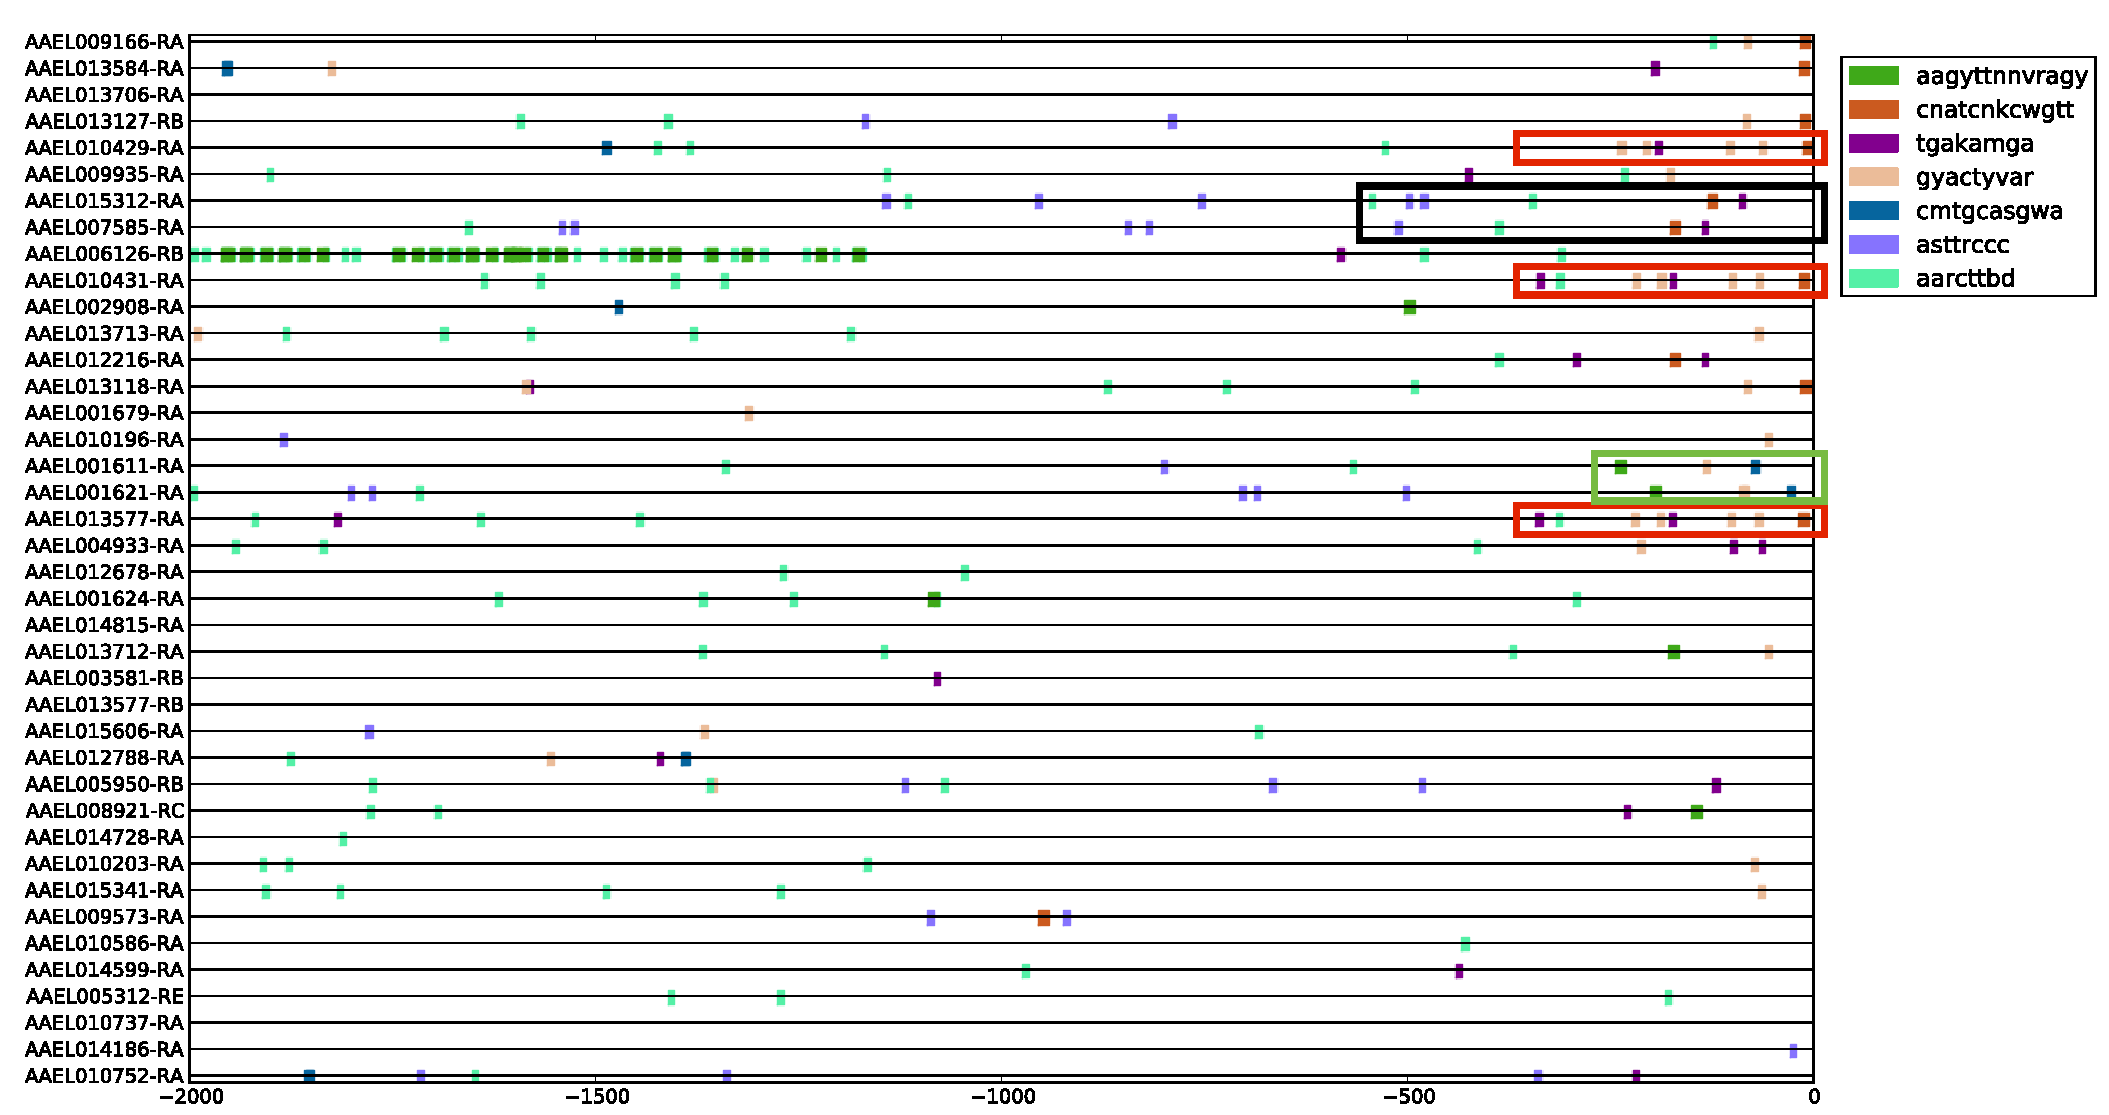
\includegraphics[width=.9\textwidth]{figures/figs/bonnizoniCREs.pdf}

\caption[Motif map of putative CREs from transcripts detected only in bloodfed female \Aa]{\sf \textbf{Motif map of putative CREs discovered by SCOPE using transcripts detected significantly only in bloodfed female \Aa:} Locations of representative SCOPE-derived CRE motifs in the 2000 bp upstream of the annotated translational start site in the 40 transcripts detected significantly only in bloodfed females. Transcript names on the left are ordered from most (top) to least (bottom) abundant.  Candidate CRMs are highlighted in like-colored rectangles.

Adapted from \cite{Bonizzoni2011}}
\label{fig:bonnizoniCREs}
\end{figure}

\section{Strain Variation in the Transcriptome of the Dengue Fever Vector, Aedes aegypti}

Figure \ref{fig:aa-diff-paralogs}

\begin{figure}[h]

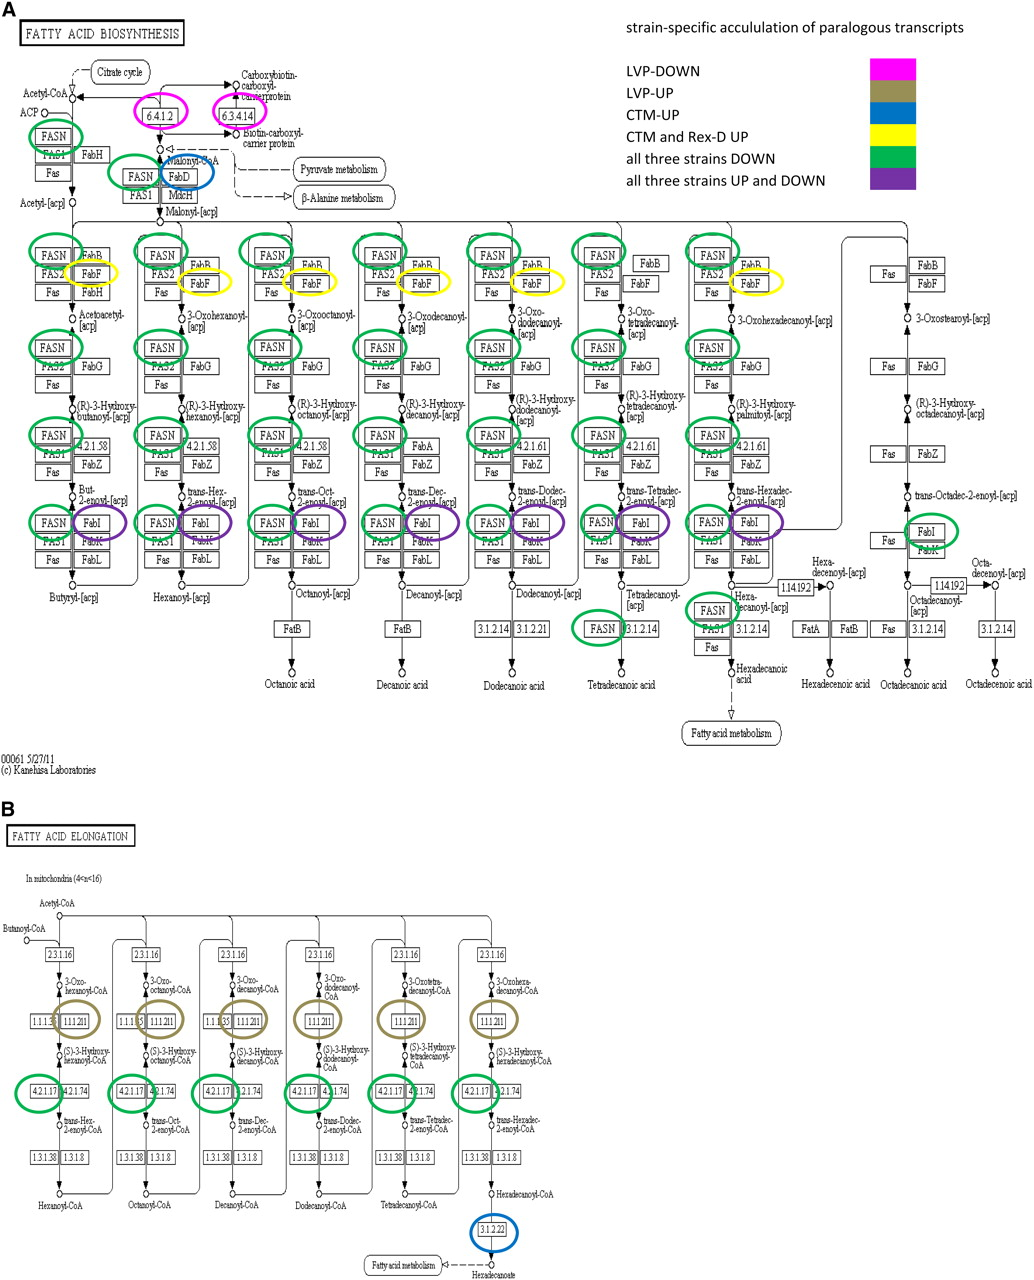
\includegraphics[width=.9\textwidth]{figures/figs/aa-diff-paralogs.jpg}

\caption[Fatty acid biosynthesis and elongation in mitochondria]{\sf \textbf{Fatty acid biosynthesis and elongation in mitochondria:} Proteins corresponding to transcripts accumulated in a strain-specific manner are circled in a color corresponding to the strain and condition defined in the legend (panels A and B).

Excerpted from \cite{bonizzoni2012strain}}
\label{fig:aa-diff-paralogs}
\end{figure}



\section{Complex modulation of the Aedes aegypti transcriptome in response to dengue virus infection}

Figure \ref{fig:bonizzoni2012complex-cre}

\begin{figure}[hp]
\centering

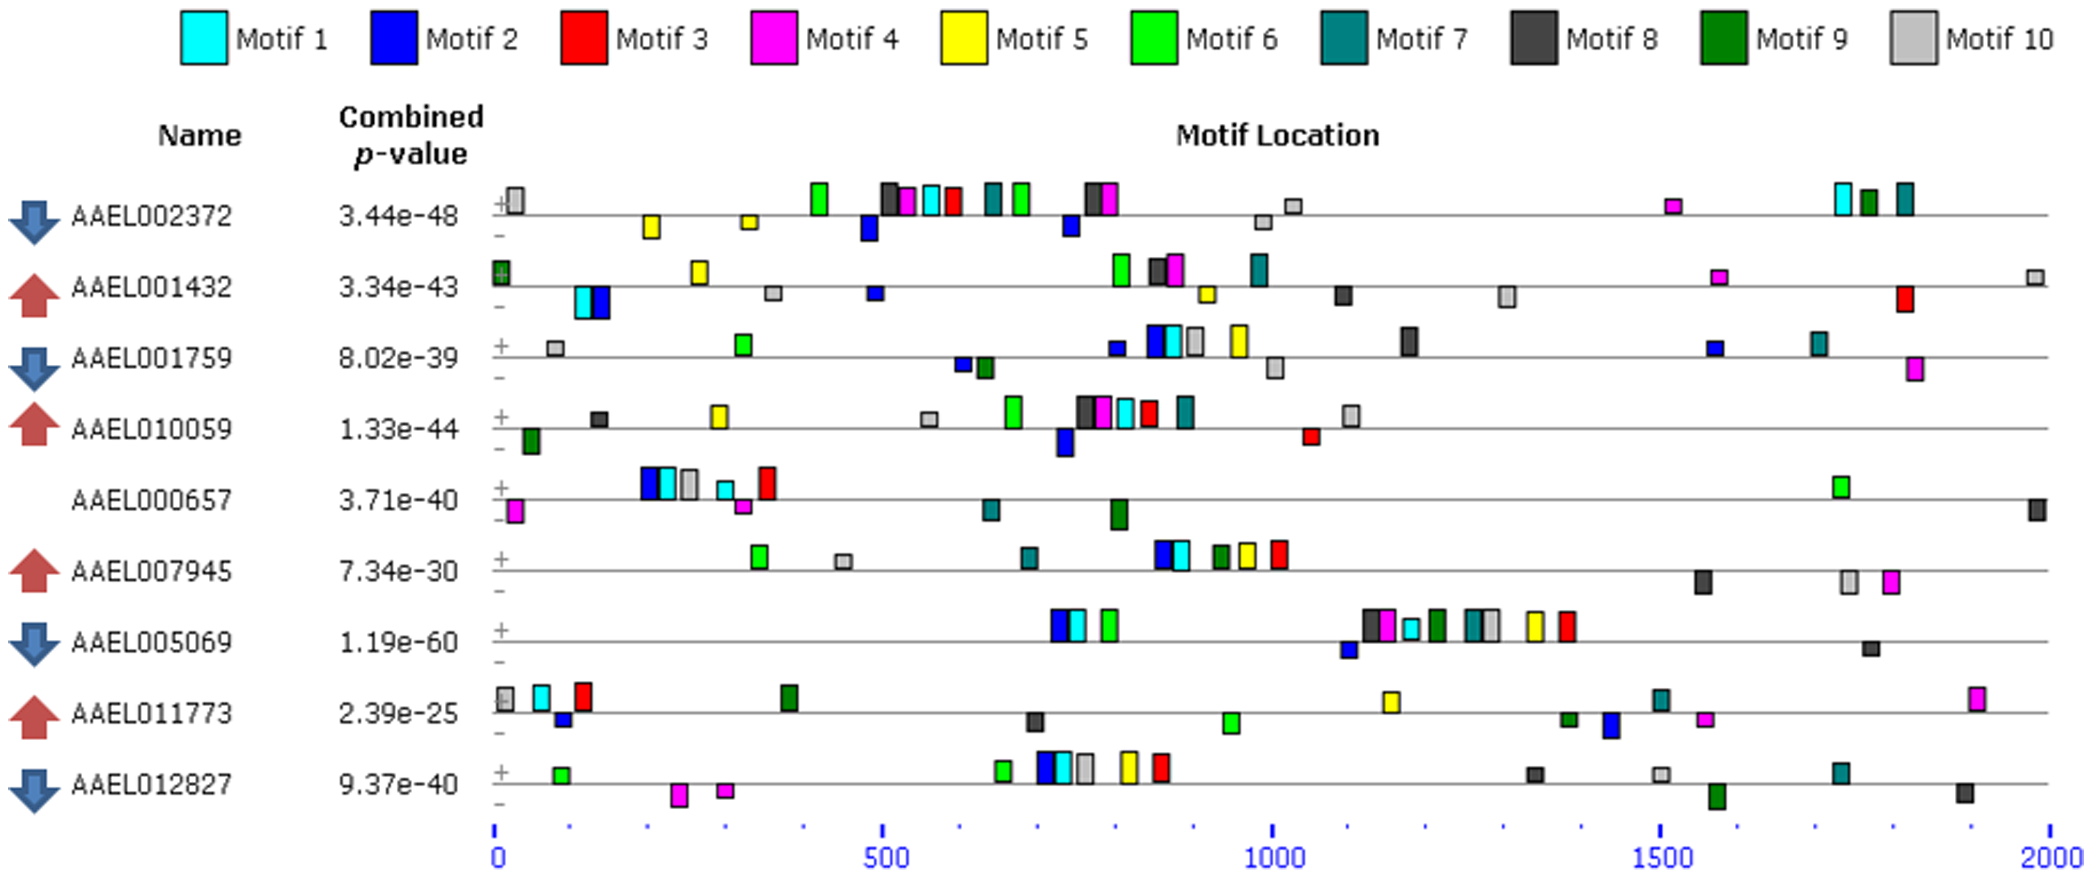
\includegraphics[width=.99\textwidth]{figures/figs/bonizzoni2012complex-cre.png}

\caption[MEME analysis of nine genes with \texorpdfstring{FPKM\textsubscript{DENVI}}{FPKM DENVI} ≥ 100 in carcasses and salivary glands at 14 dpi]{\sf \textbf{MEME analysis of nine genes with \texorpdfstring{FPKM\textsubscript{DENVI}}{FPKM DENVI} ≥ 100 in carcasses and salivary glands at 14 dpi} These genes also were identified with transcripts exhibiting significant differential accumulation in analyses of salivary gland samples of the Liverpool strain infected with DEV2 Thailand 16881 [26]. Colored boxes represent individual putative CREs and their locations in promoters of each gene. Red and blue arrows adjacent to Ensembl Gene ID indicate those genes whose transcripts were detected previously as more or less abundant following DENV infection [26]. Distances in base-pairs are provided below the schematic of each gene.
doi:10.1371/journal.pone.0050512.g004

Excerpted from \cite{bonizzoni2012complex}}
\label{fig:bonizzoni2012complex-cre}
\end{figure}

% \texorpdfstring{FPKM\textsubscript{DENVI}}{FPKM DENVI}


\section{\texorpdfstring{like\textsubscript{this}}{like this}}

%%% Local Variables: ***
%%% mode: latex ***
%%% TeX-master: "thesis.tex" ***
%%% End: ***

% Figure / table inputs

\chapter{Approach and Custom Software solutions}
\todo[inline]{replace CITEME tags in Approach and Custom Software solutions}

\section{Purpose}
Illustrate how lessons learned in previous chapter (as well as new lessons introduced here) are addressed through custom software solutions.
\begin{enumerate}
 \item RNA-seq analysis, reproducibility, updating
 \item Integration of multiple disparate Omics scale data types
 \item Documentation of exactly how analyses were carried out (IPython notebooks)
\end{enumerate}

\todo[inline]{MEGA: you need to write most of this chapter}

\section{The phylogenetic transcriptional correspondence index (PTCI)}








Look at the parameter space of the PTCI (Figure \ref{fig:ptci-space}).  




\begin{figure}[hp]
\centering
  \begin{subfigure}[b]{.9\linewidth}
    \centering

    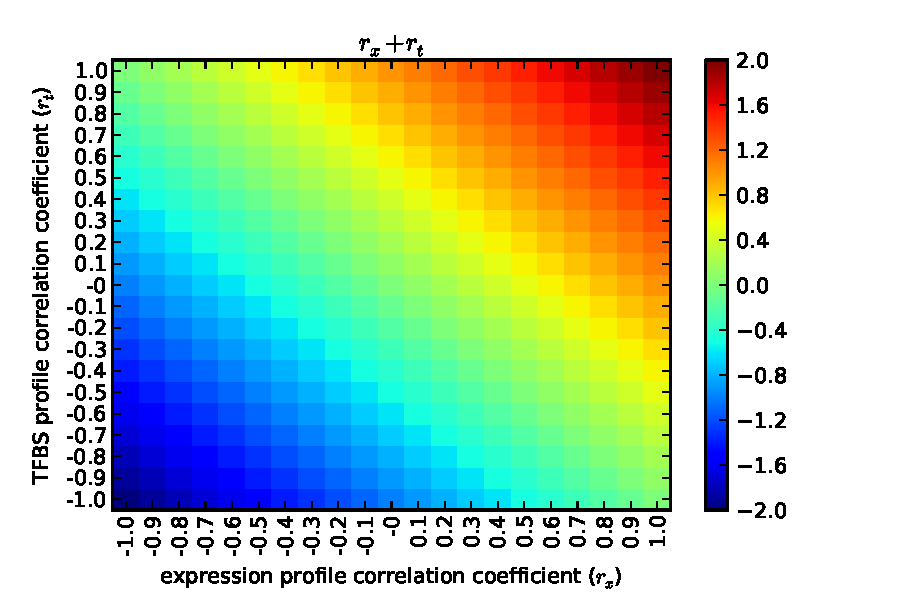
\includegraphics[width=.9\linewidth]{figures/figs/thesis-xprn-tfbs.pdf}
    \caption{}
    \label{fig:ptci-space-a}
  \end{subfigure}%

  

  \begin{subfigure}[b]{.9\linewidth}
    \centering

    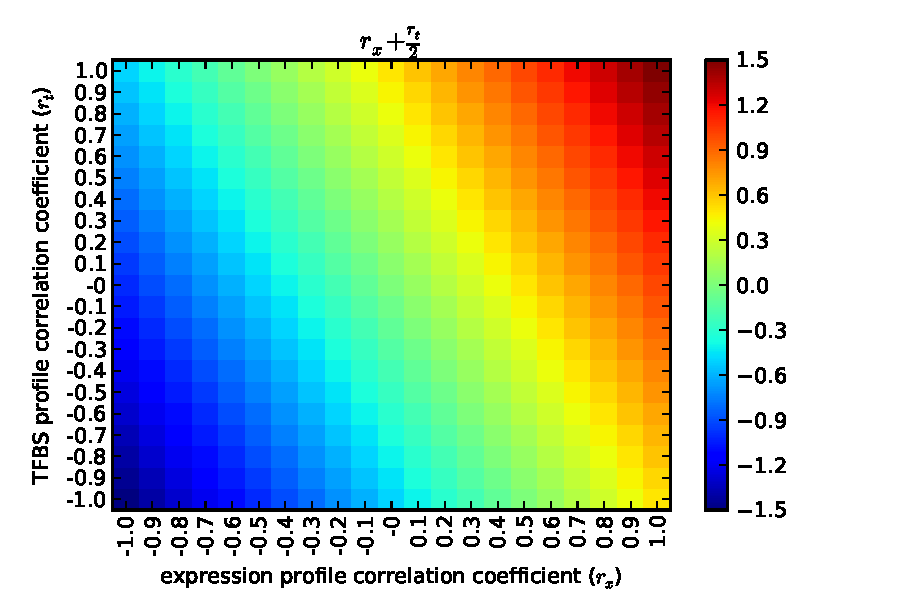
\includegraphics[width=.9\linewidth]{figures/figs/thesis-xprn-scaled-tfbs.pdf}
    \caption{}
    \label{fig:ptci-space-b}
  \end{subfigure}

\caption[Exploring the parameter space of the expression and TFBS components of the PTCI]{\sf \textbf{Exploring the parameter space of the expression and TFBS components of the PTCI:} \\
\textbf{(A)} The expression and TFBS profile correlations each carry the same weight.  TFBS data is not strictly empirical, and position weight matrix models inherently are prone to produce false positive predictions. Here, each correlation-type exerts equal influence on the final score assigned to the ortholog relationship.  \textbf{(B)} The TFBS profile correlation is penalized due to the non-empirical nature and expected false positive information it contains. Here, TFBS profile data contributes to the final score at most 50\% as much as expression data.}
\label{fig:ptci-space}
\end{figure}

Here is the PTCI calculation:


\begin{equation} \label{eq:ptci}
PTCI = ( r_{x} + \frac{r_{t}}{2} ) \cdot w(d)
\end{equation}


The graph model is useful (Figure \ref{fig:nway-ortholog-graph})


\begin{figure}[hp]
\centering
% 
    \begin{subfigure}[t]{.5\linewidth}
    \centering
    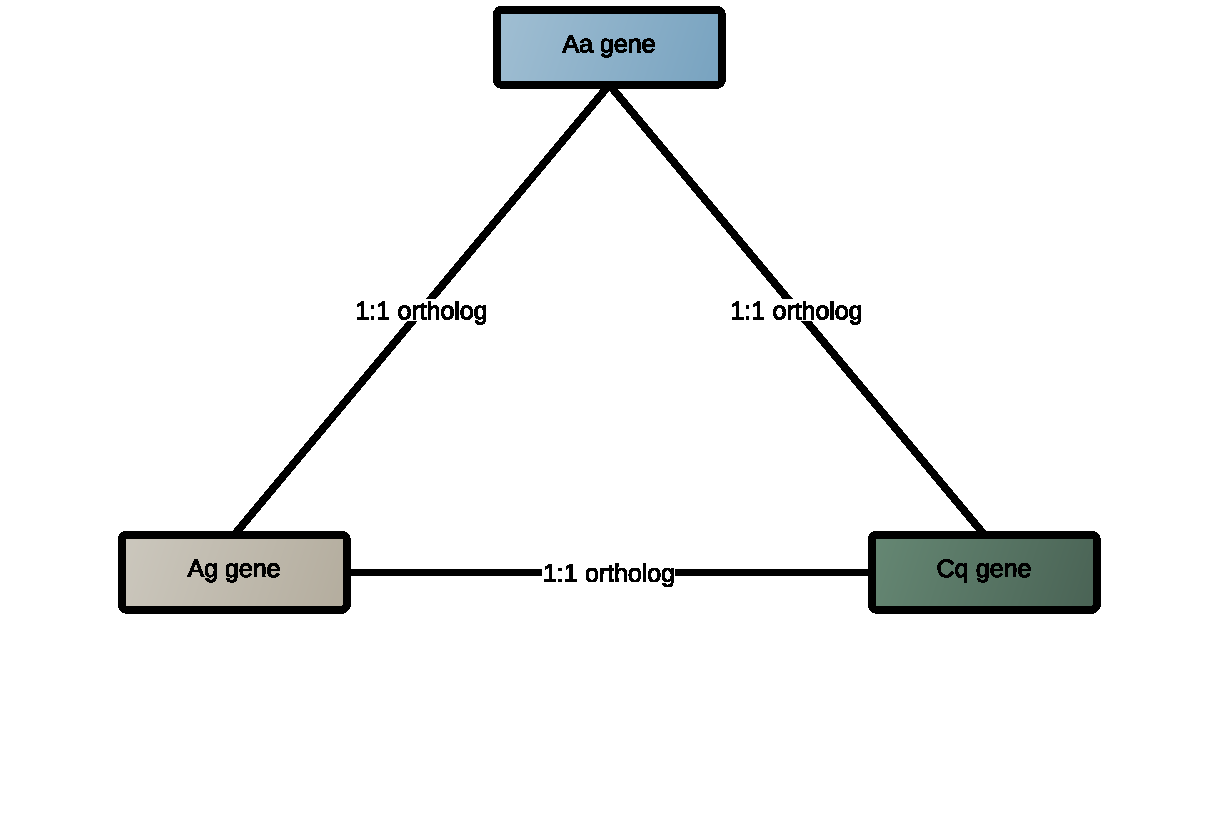
\includegraphics[width=\linewidth]{figures/figs/gfunc_graph_figs/ortho-graph-model.pdf}
    \caption{N-way 1:1 ortholog graph structure}\label{fig:nway-ortholog-graph-model}
    \end{subfigure}%
% 
% 
% 
    \begin{subfigure}[t]{.5\linewidth}
    \centering
    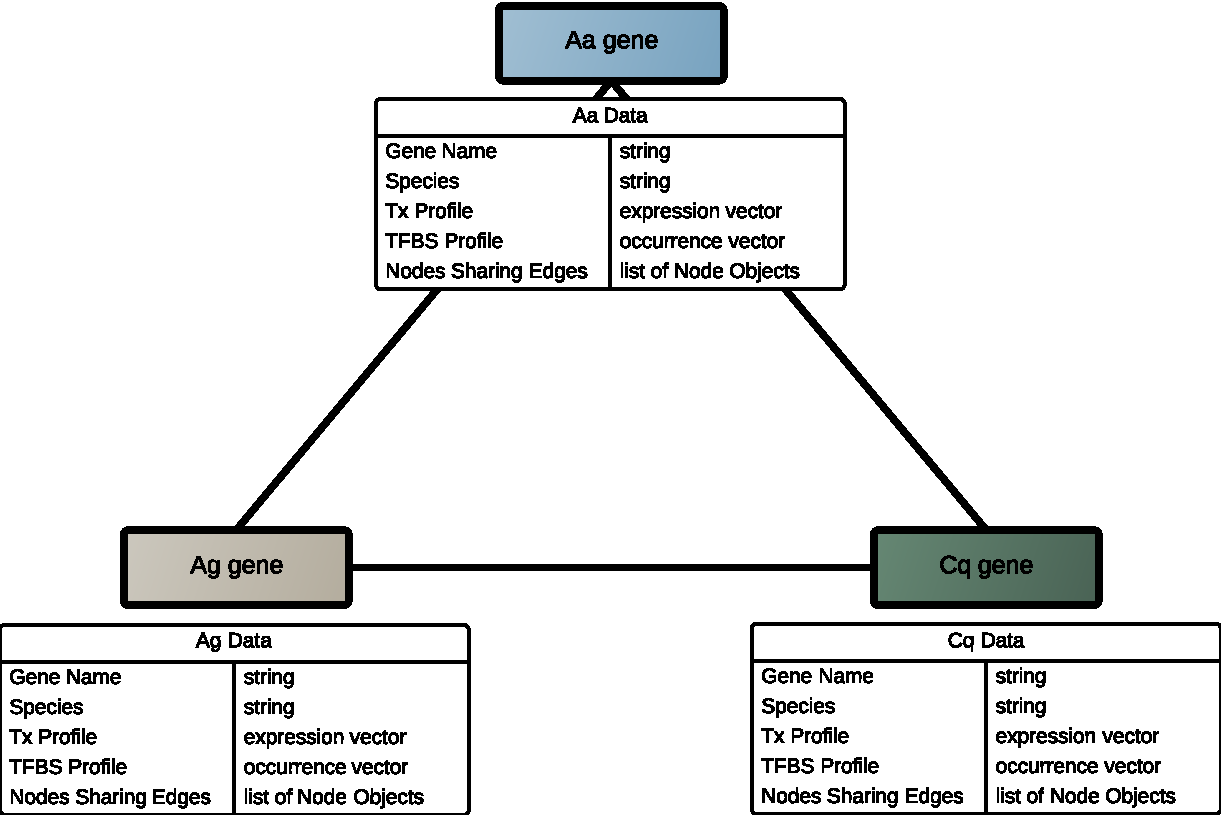
\includegraphics[width=\linewidth]{figures/figs/gfunc_graph_figs/ortho-graph-node-data.pdf}
    \caption{Node data model}\label{fig:nway-ortholog-graph-node-data}
    \end{subfigure}
% 
% 
% 
% 
% 
% 
    \begin{subfigure}[t]{.5\linewidth}
    \centering
    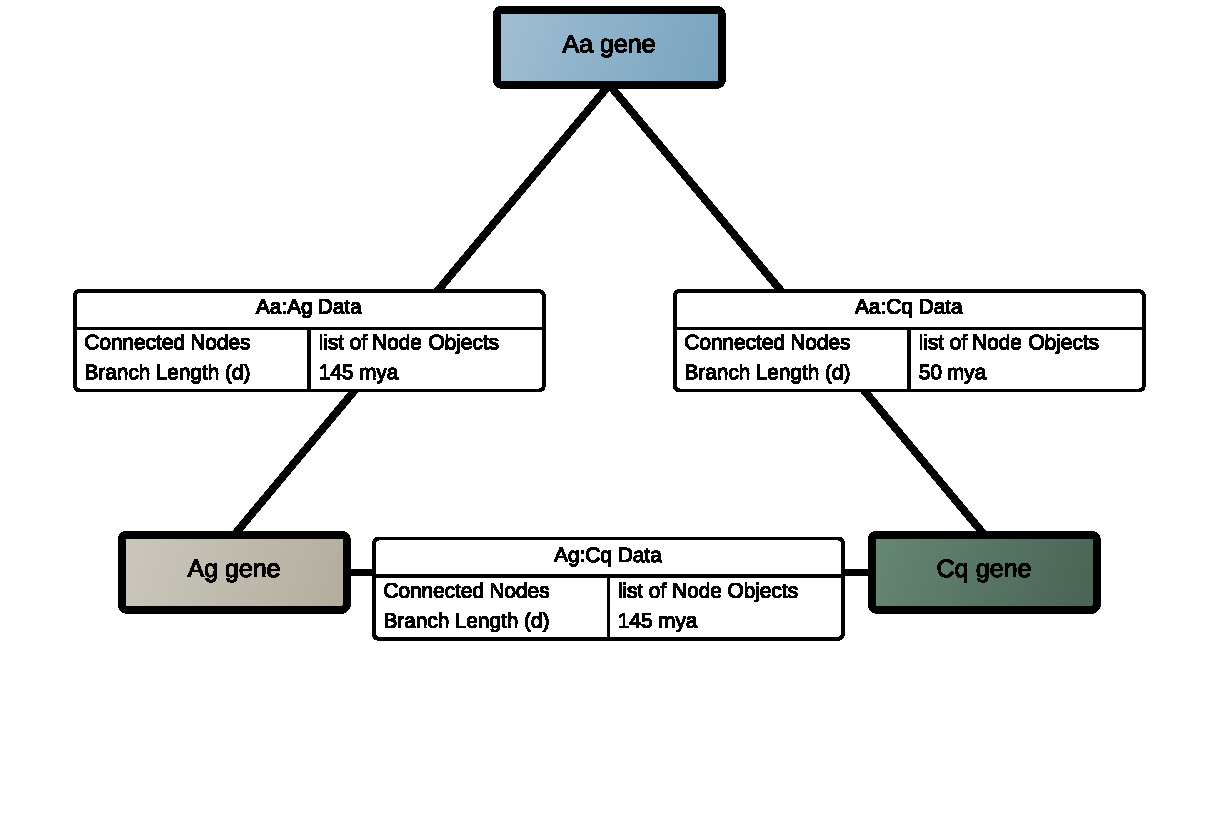
\includegraphics[width=\linewidth]{figures/figs/gfunc_graph_figs/ortho-graph-edge-data.pdf}
    \caption{Edge data model}\label{fig:nway-ortholog-graph-edge-data}
    \end{subfigure}%
% 
% 
%     
    \begin{subfigure}[t]{.5\linewidth}
    \centering
    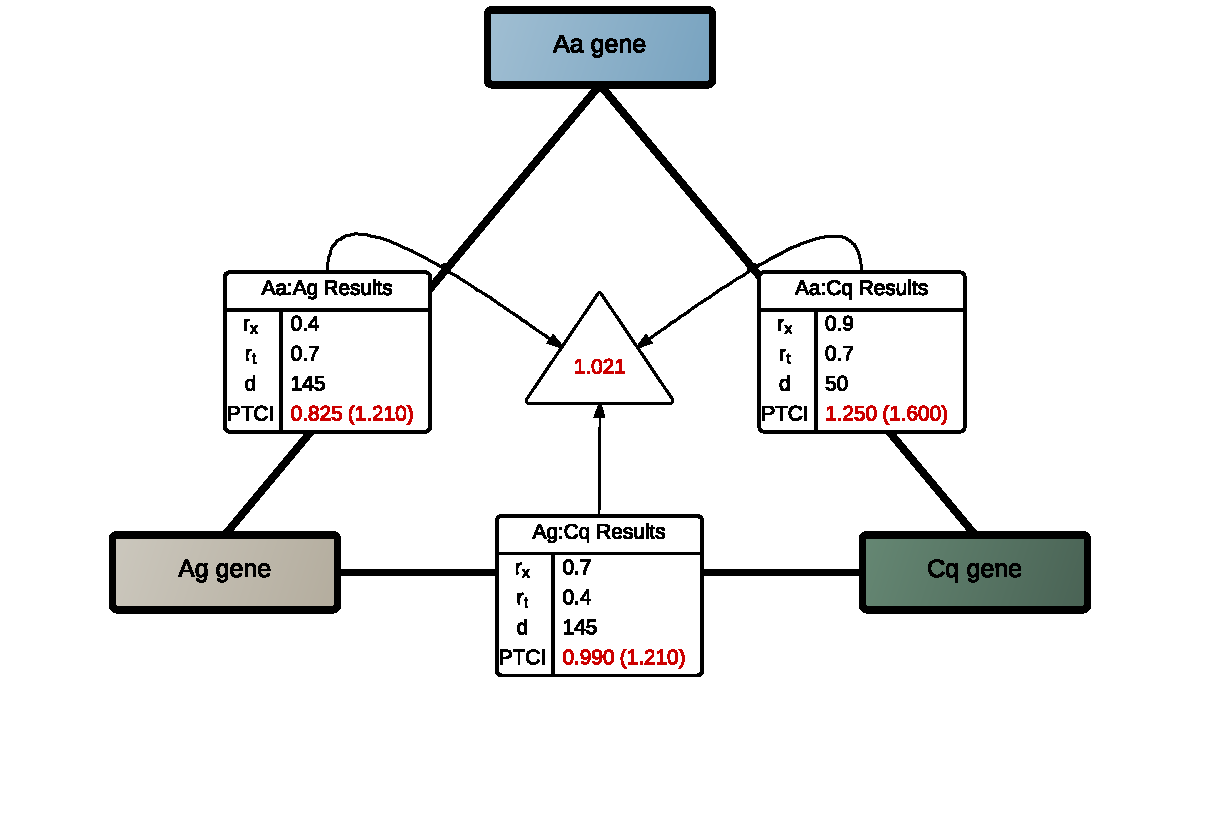
\includegraphics[width=\linewidth]{figures/figs/gfunc_graph_figs/ortho-graph-ptci.pdf}
    \caption{Example PTCI data}\label{fig:nway-ortholog-graph-ptci}
    \end{subfigure}
% 
% 
% 
\caption[Graph model used to integrate data types]{\sf \textbf{Graph model used to integrate data types.}}\label{fig:nway-ortholog-graph}
\end{figure}


\pagebreak[4]
\section{Blacktie RNA-seq pipeline}

See Figure \ref{fig:tuxedo}




\begin{landscape}
 
 
 \begin{figure}[hp]
\centering
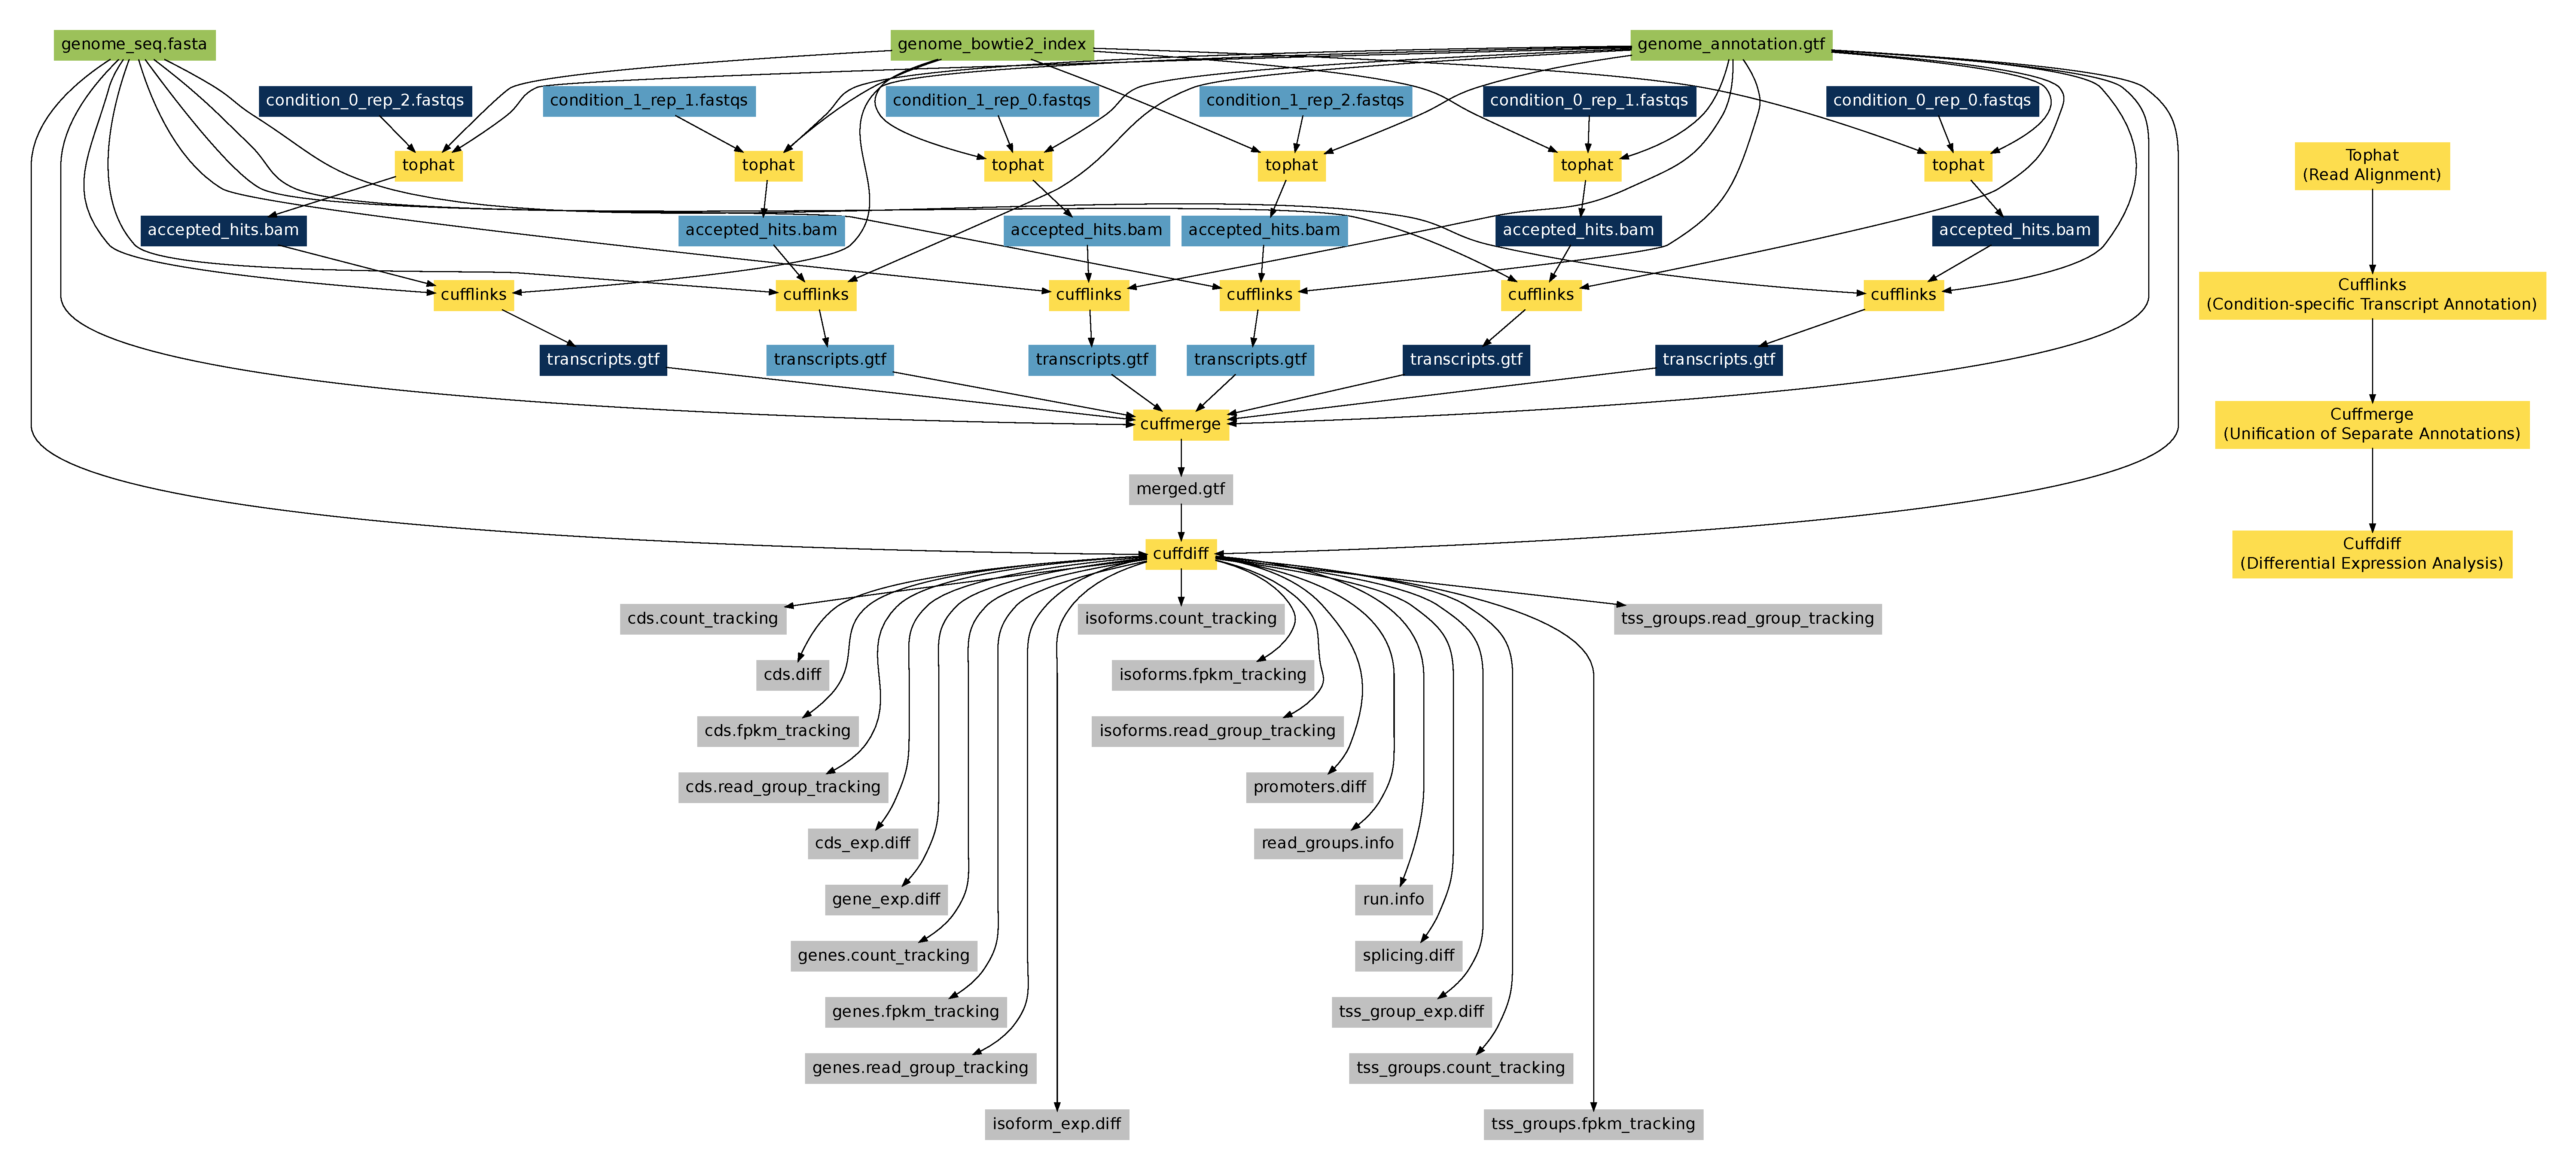
\includegraphics[width=\linewidth]{figures/figs/tuxedo_dot/707354_6/tophat_cufflinks_ins_outs.pdf}
\caption[Diagram of Abbreviated Tophat/Cufflinks Inputs and Outputs]{\sf \textbf{Diagram of Abbreviated Tophat/Cufflinks Inputs and Outputs:}\\
	This figure demonstrates the complexities of a typical RNA-seq experiment as analyzed with the \gls{TuxProt}. It models a fairly \textbf{simple} two condition experiment with each condition having three replications. It is ``abbreviated'' in that it only displays the output files that will be used in the next step for all steps except the \UseVerb{cuffdiff} step. The complete output of \UseVerb{cuffdiff} is included to demonstrate the final challenge of integrating the data which exists in multiple cross-referenced files.\\ 
	(\emph{Dark Blue} - Inputs/Outputs associated with Condition Zero; 
	\emph{Light Blue} - Inputs/Outputs associated with Condition One; 
	\emph{Grey} - Inputs/Outputs associated with Condition Zero \textbf{AND} Condition One; 
	\emph{Green} - Inputs Specific to the Reference Genome; 
	\emph{Gold} - Program Calls)
}
	\label{fig:tuxedo}
\end{figure}
 
 
 
\end{landscape}






%%% Local Variables: ***
%%% mode: latex ***
%%% TeX-master: "thesis.tex" ***
%%% End: ***

\chapter{Analysis of Conservation of Midgut Transcriptional Response to Bloodfeeding in Four Vector Mosquitoes}
\todo[inline]{replace CITEME tags in Analysis of Conservation of Midgut Transcriptional Response to Bloodfeeding in Four Vector Mosquitoes}

\todo[inline]{write all the figures}

\todo[inline]{MEGA: you need to write most of this chapter}

\section{Background}
\begin{enumerate}
 \item Biological importance of bloodmeal to mosquito
 \item Biological importance of bloodmeal to transmission cyc
\end{enumerate}



\begin{figure}[hp]
% 
\begin{subfigure}[t]{.5\linewidth}
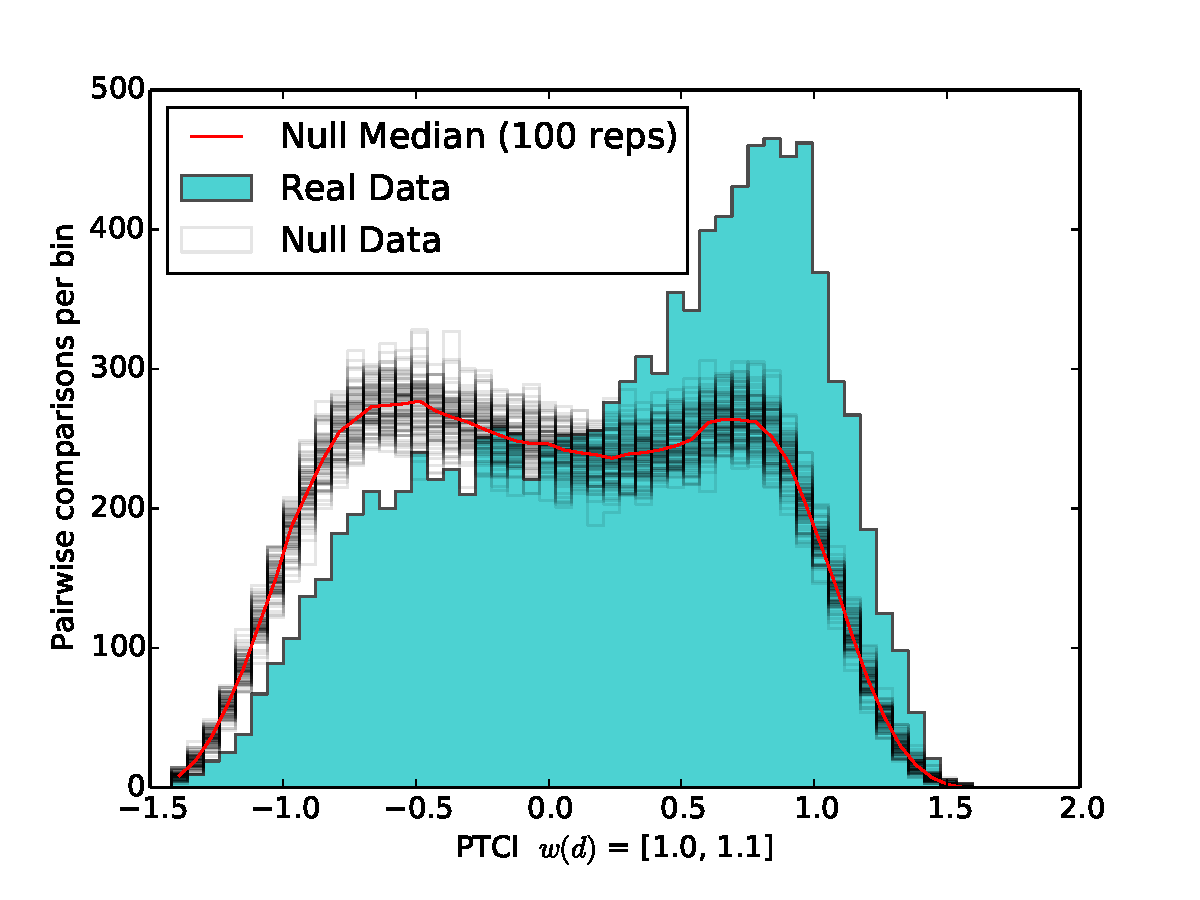
\includegraphics[width=\linewidth]{/home/gus/Dropbox/repos/git/uci-thesis-latex/figures/figs/ecr_team_ptci/pairwise_ptci_hist.pdf}
\caption{}
\label{fig:pairwise-ptci-hists-base}
\end{subfigure}%
\quad
\begin{subfigure}[t]{.5\linewidth}
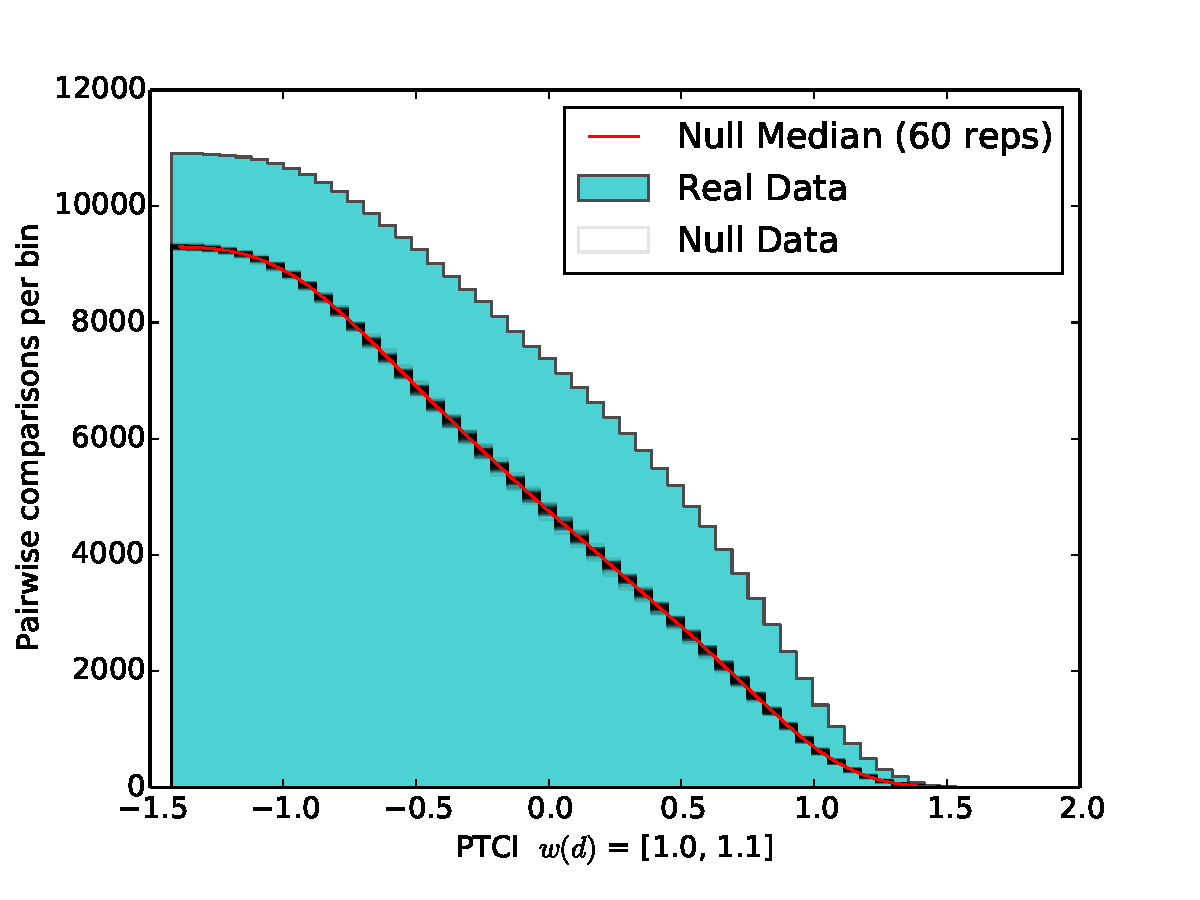
\includegraphics[width=\linewidth]{/home/gus/Dropbox/repos/git/uci-thesis-latex/figures/figs/ecr_team_ptci/pairwise_ptci_cum_hist.pdf}
\caption{}
\label{fig:pairwise-ptci-hists-rcum-hist}
\end{subfigure}
% 
\begin{subfigure}[t]{.5\linewidth}
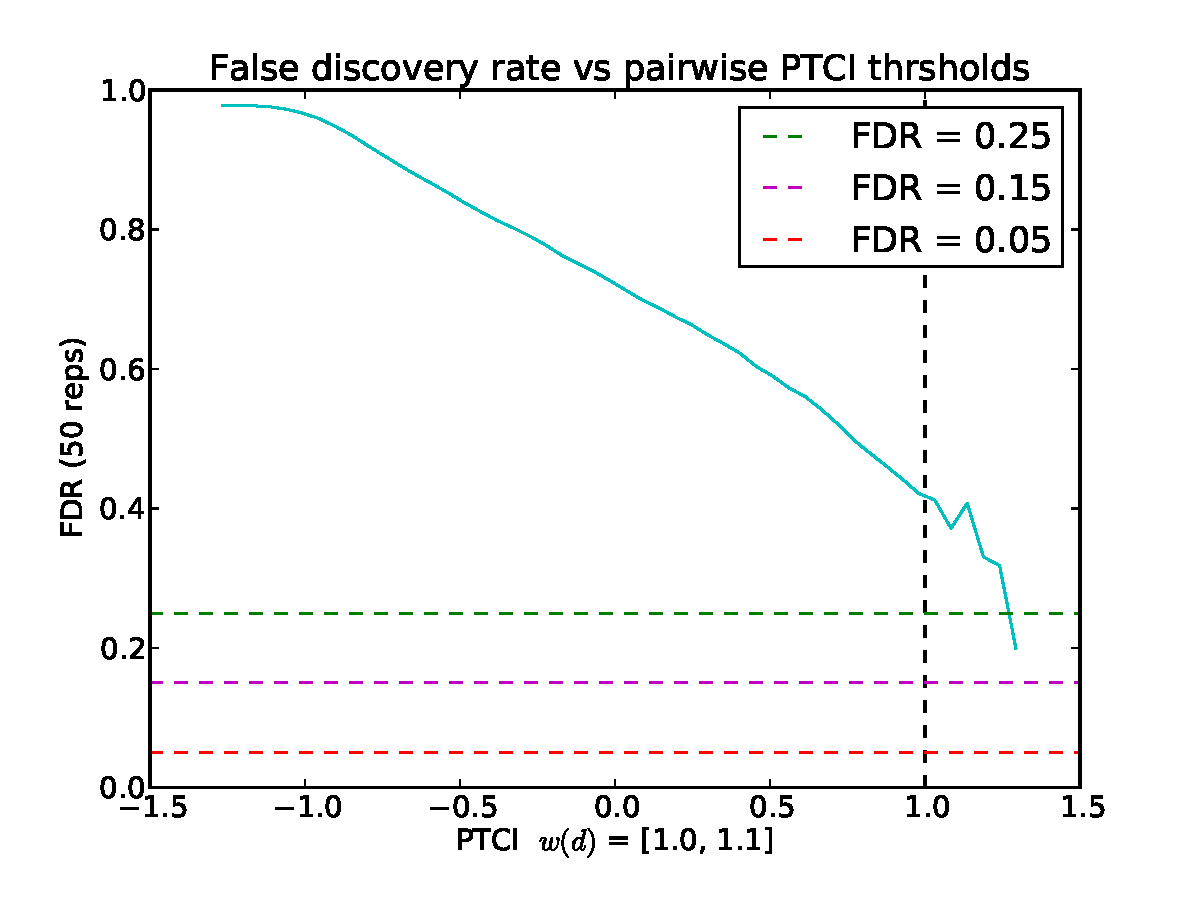
\includegraphics[width=\linewidth]{/home/gus/Dropbox/repos/git/uci-thesis-latex/figures/figs/ecr_team_ptci/pairwise_ptci_fdr.pdf}
\caption{}
\label{fig:pairwise-ptci-hists-fdr}
\end{subfigure}
% 
\caption[Pairwise PTCI results]{\sf \textbf{Pairwise PTCI results}:\\
\textbf{(A)} Histogram of pairwise PTCI results vs null distributions.
\textbf{(B)} Reverse Cumulative histogram of pairwise PTCI results vs null distributions.
\textbf{(C)} False discover rate vs PTCI threshold.}
\label{fig:pairwise-ptci-hists}
\end{figure}
Figure \ref{fig:pairwise-ptci-hists}


\begin{figure}[hp]
%
\subcaptionbox{\label{fig:mean-ptci-hists-base}}
{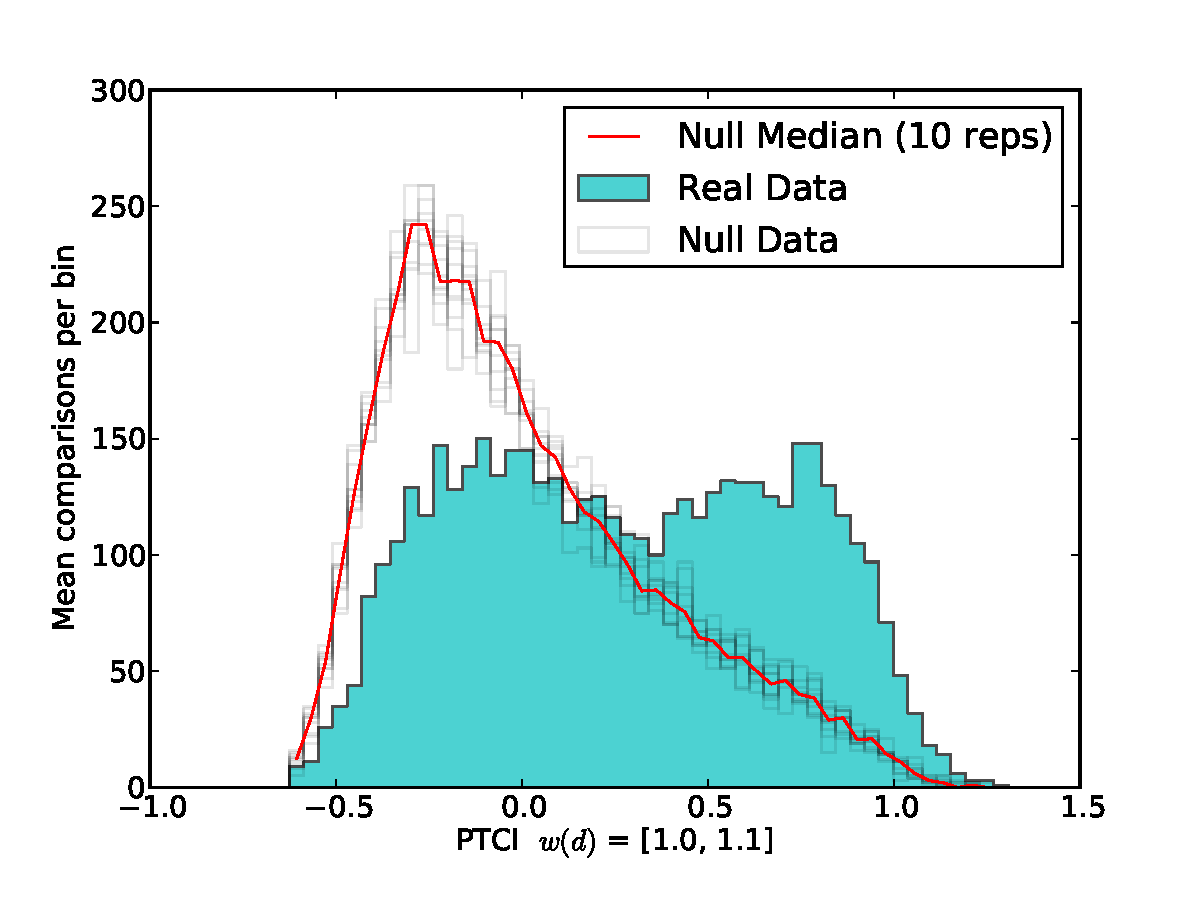
\includegraphics[width=.5\linewidth]{figures/figs/ecr_team_ptci/mean_ptci_hist.pdf}}
% 
\subcaptionbox{\label{fig:mean-ptci-hists-rcum-hist}}
{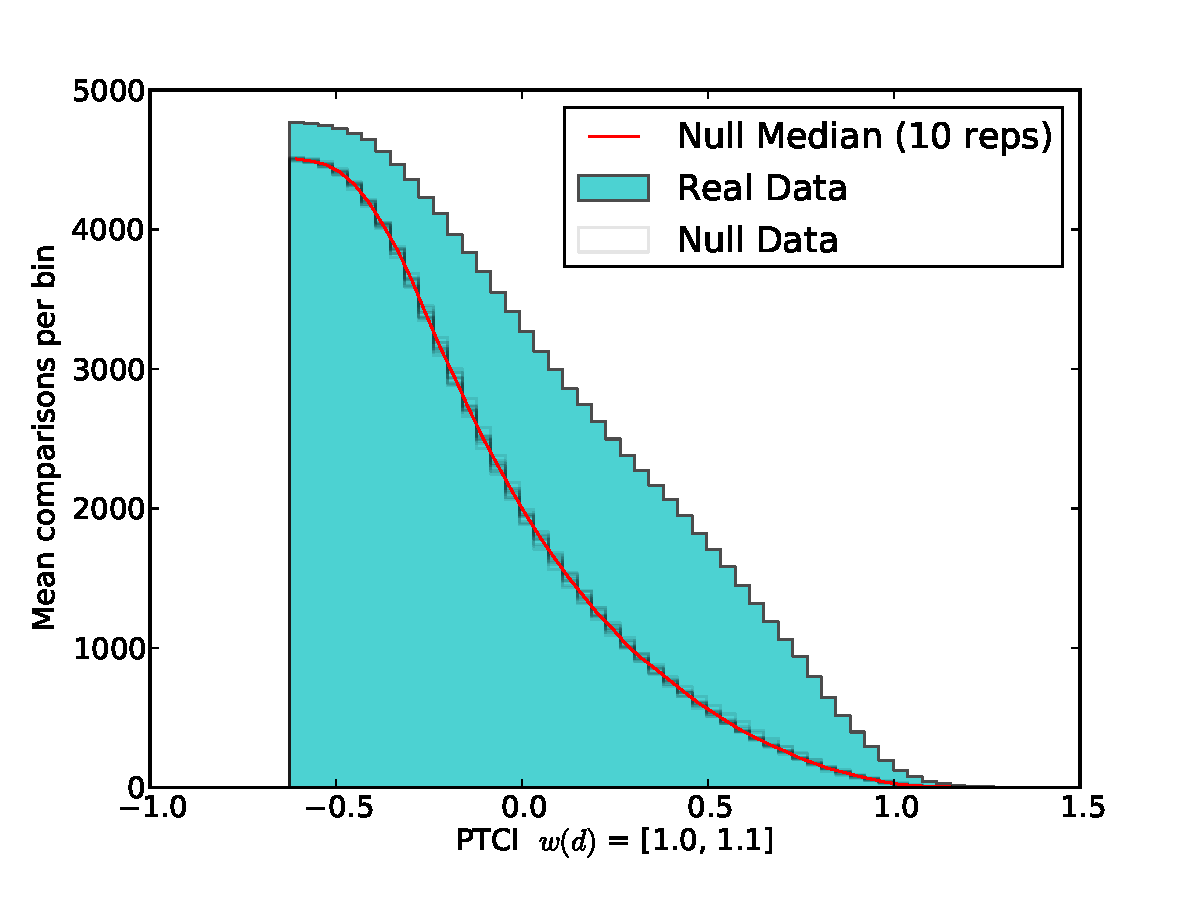
\includegraphics[width=.5\linewidth]{figures/figs/ecr_team_ptci/mean_ptci_cum_hist.pdf}}
% 
\subcaptionbox{\label{fig:mean-ptci-hists-fdr}}
{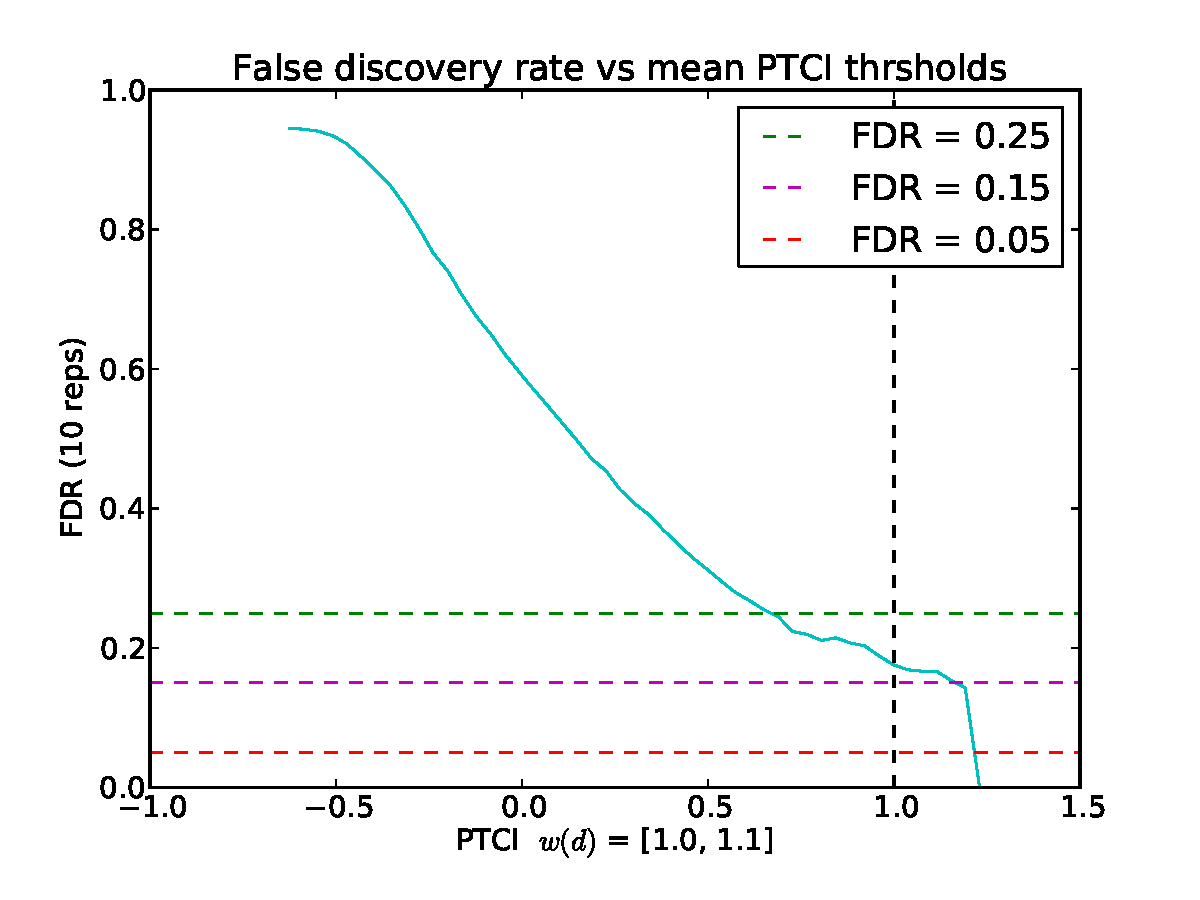
\includegraphics[width=.5\linewidth]{figures/figs/ecr_team_ptci/mean_ptci_fdr.pdf}}
% 
% 
\caption[Mean PTCI results]{\sf \textbf{Mean PTCI results}:\\
\textbf{(A)} Histogram of mean PTCI results vs null distributions.
\textbf{(B)} Reverse Cumulative histogram of mean PTCI results vs null distributions.
\textbf{(C)} False discover rate vs PTCI threshold.}
\label{fig:mean-ptci-hists}
\end{figure}
Figure \ref{fig:mean-ptci-hists}



\begin{landscape}

    \begin{figure}[h]
    \centering
    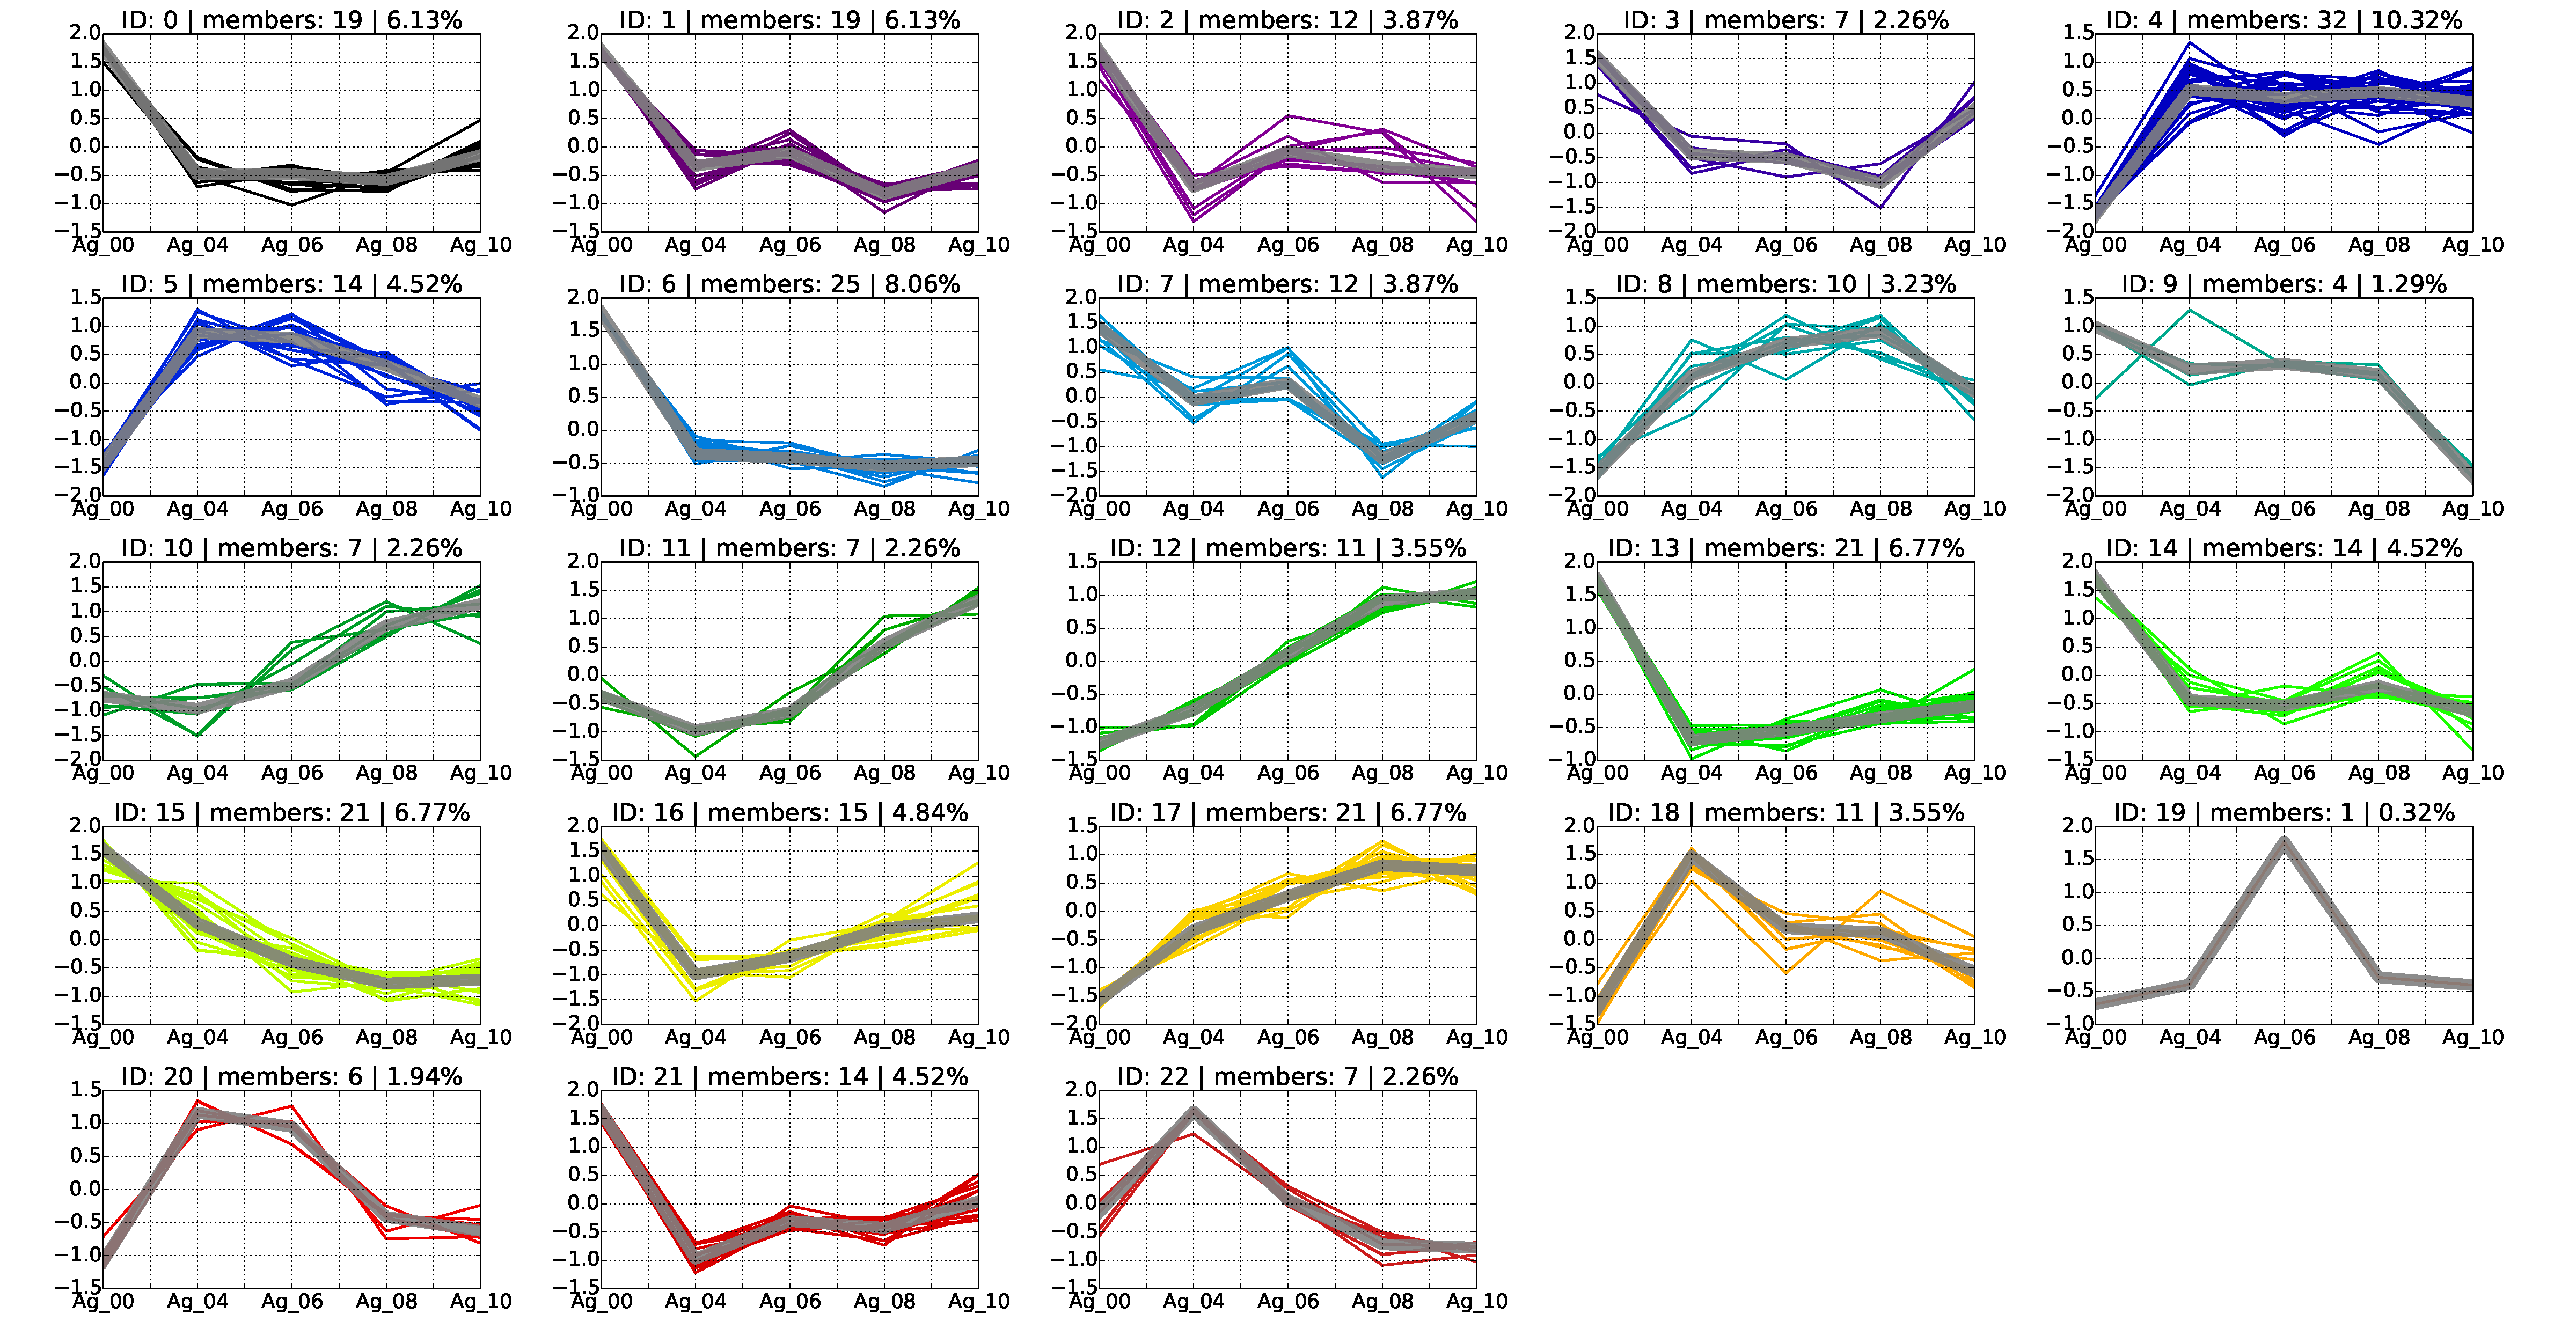
\includegraphics[width=\linewidth]{figures/figs/ecr_and_insects_ptci_20130918_orthodb7/23clusters_ptci_0_95_orthodb7.pdf}
    \caption[\Ag\ clustered abundance profiles]{\sf \textbf{\Ag\ clustered abundance profiles.} \\ 
    Clusters were generated using k-means clustering as implemented in Biopython version 1.62 \cite{Cock2009}.  Abundance profile data was log transformed after one FPKM was added to all data to remove zeros ($log_{10}(\mathrm{FPKM}+1)$).  K-means was then applied using the arithmetic mean as the center for cluster definition.  The data displayed here is the gene-wise standardization of the \textbf{raw} FPKM data such that each profile has mean = 0 and standard deviation = 1. Each median abundance profile is marked by a thick gray line. \textbf{Panel Titles} - ID: cluster identifier | members: number of genes in cluster | percentage of genes represented in all clusters. \textbf{Time Points} - \gls{NBF}, 4, 6, 8, 10 h \gls{PBM}.
}
    \label{fig:23-clusters}
    \end{figure}
    
\end{landscape}


Figure \ref{fig:23-clusters}

% 
\begin{figure}[hp]
% 
\subcaptionbox{\label{fig:cluster6-Aa}}
{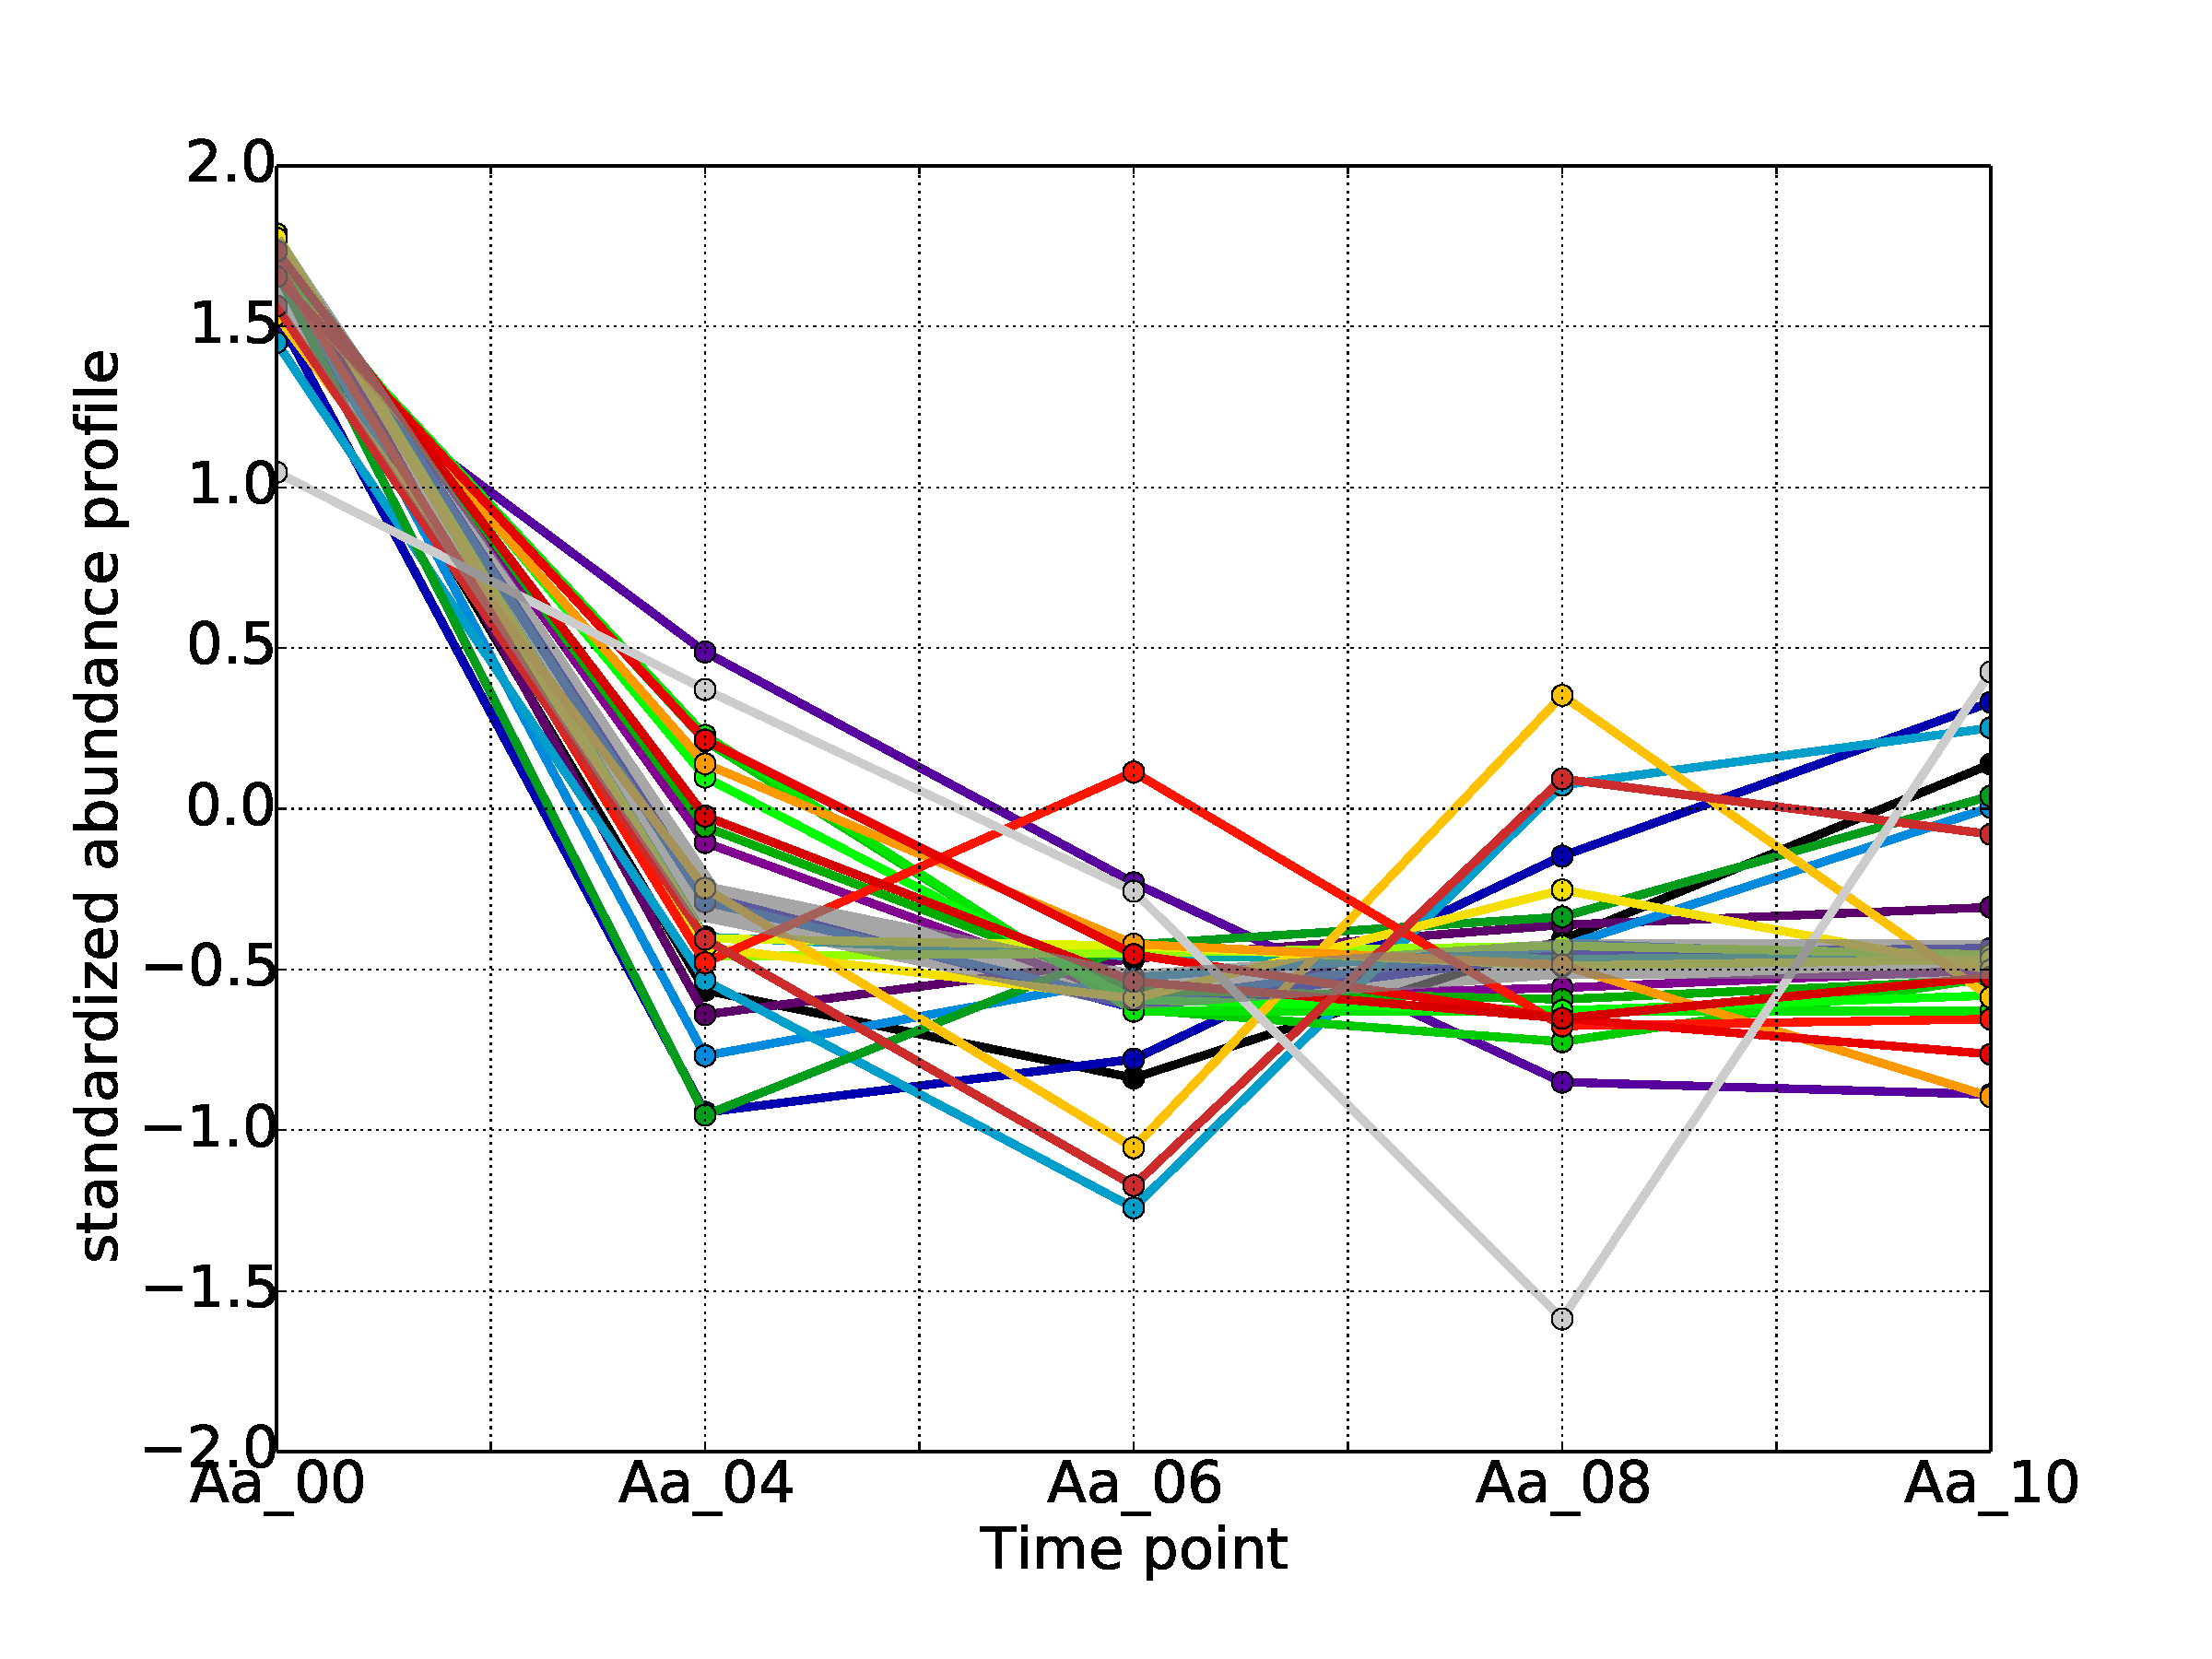
\includegraphics[width=.5\linewidth]{figures/figs/ecr_and_insects_ptci_20130918_orthodb7/downAfter4_gene_profiles_from_cummerbund/Aa_downAfter4_cls6_Ag_target_FPKMs_vb_orthos.pdf}}
%
\subcaptionbox{\label{fig:cluster6-Ag}}
{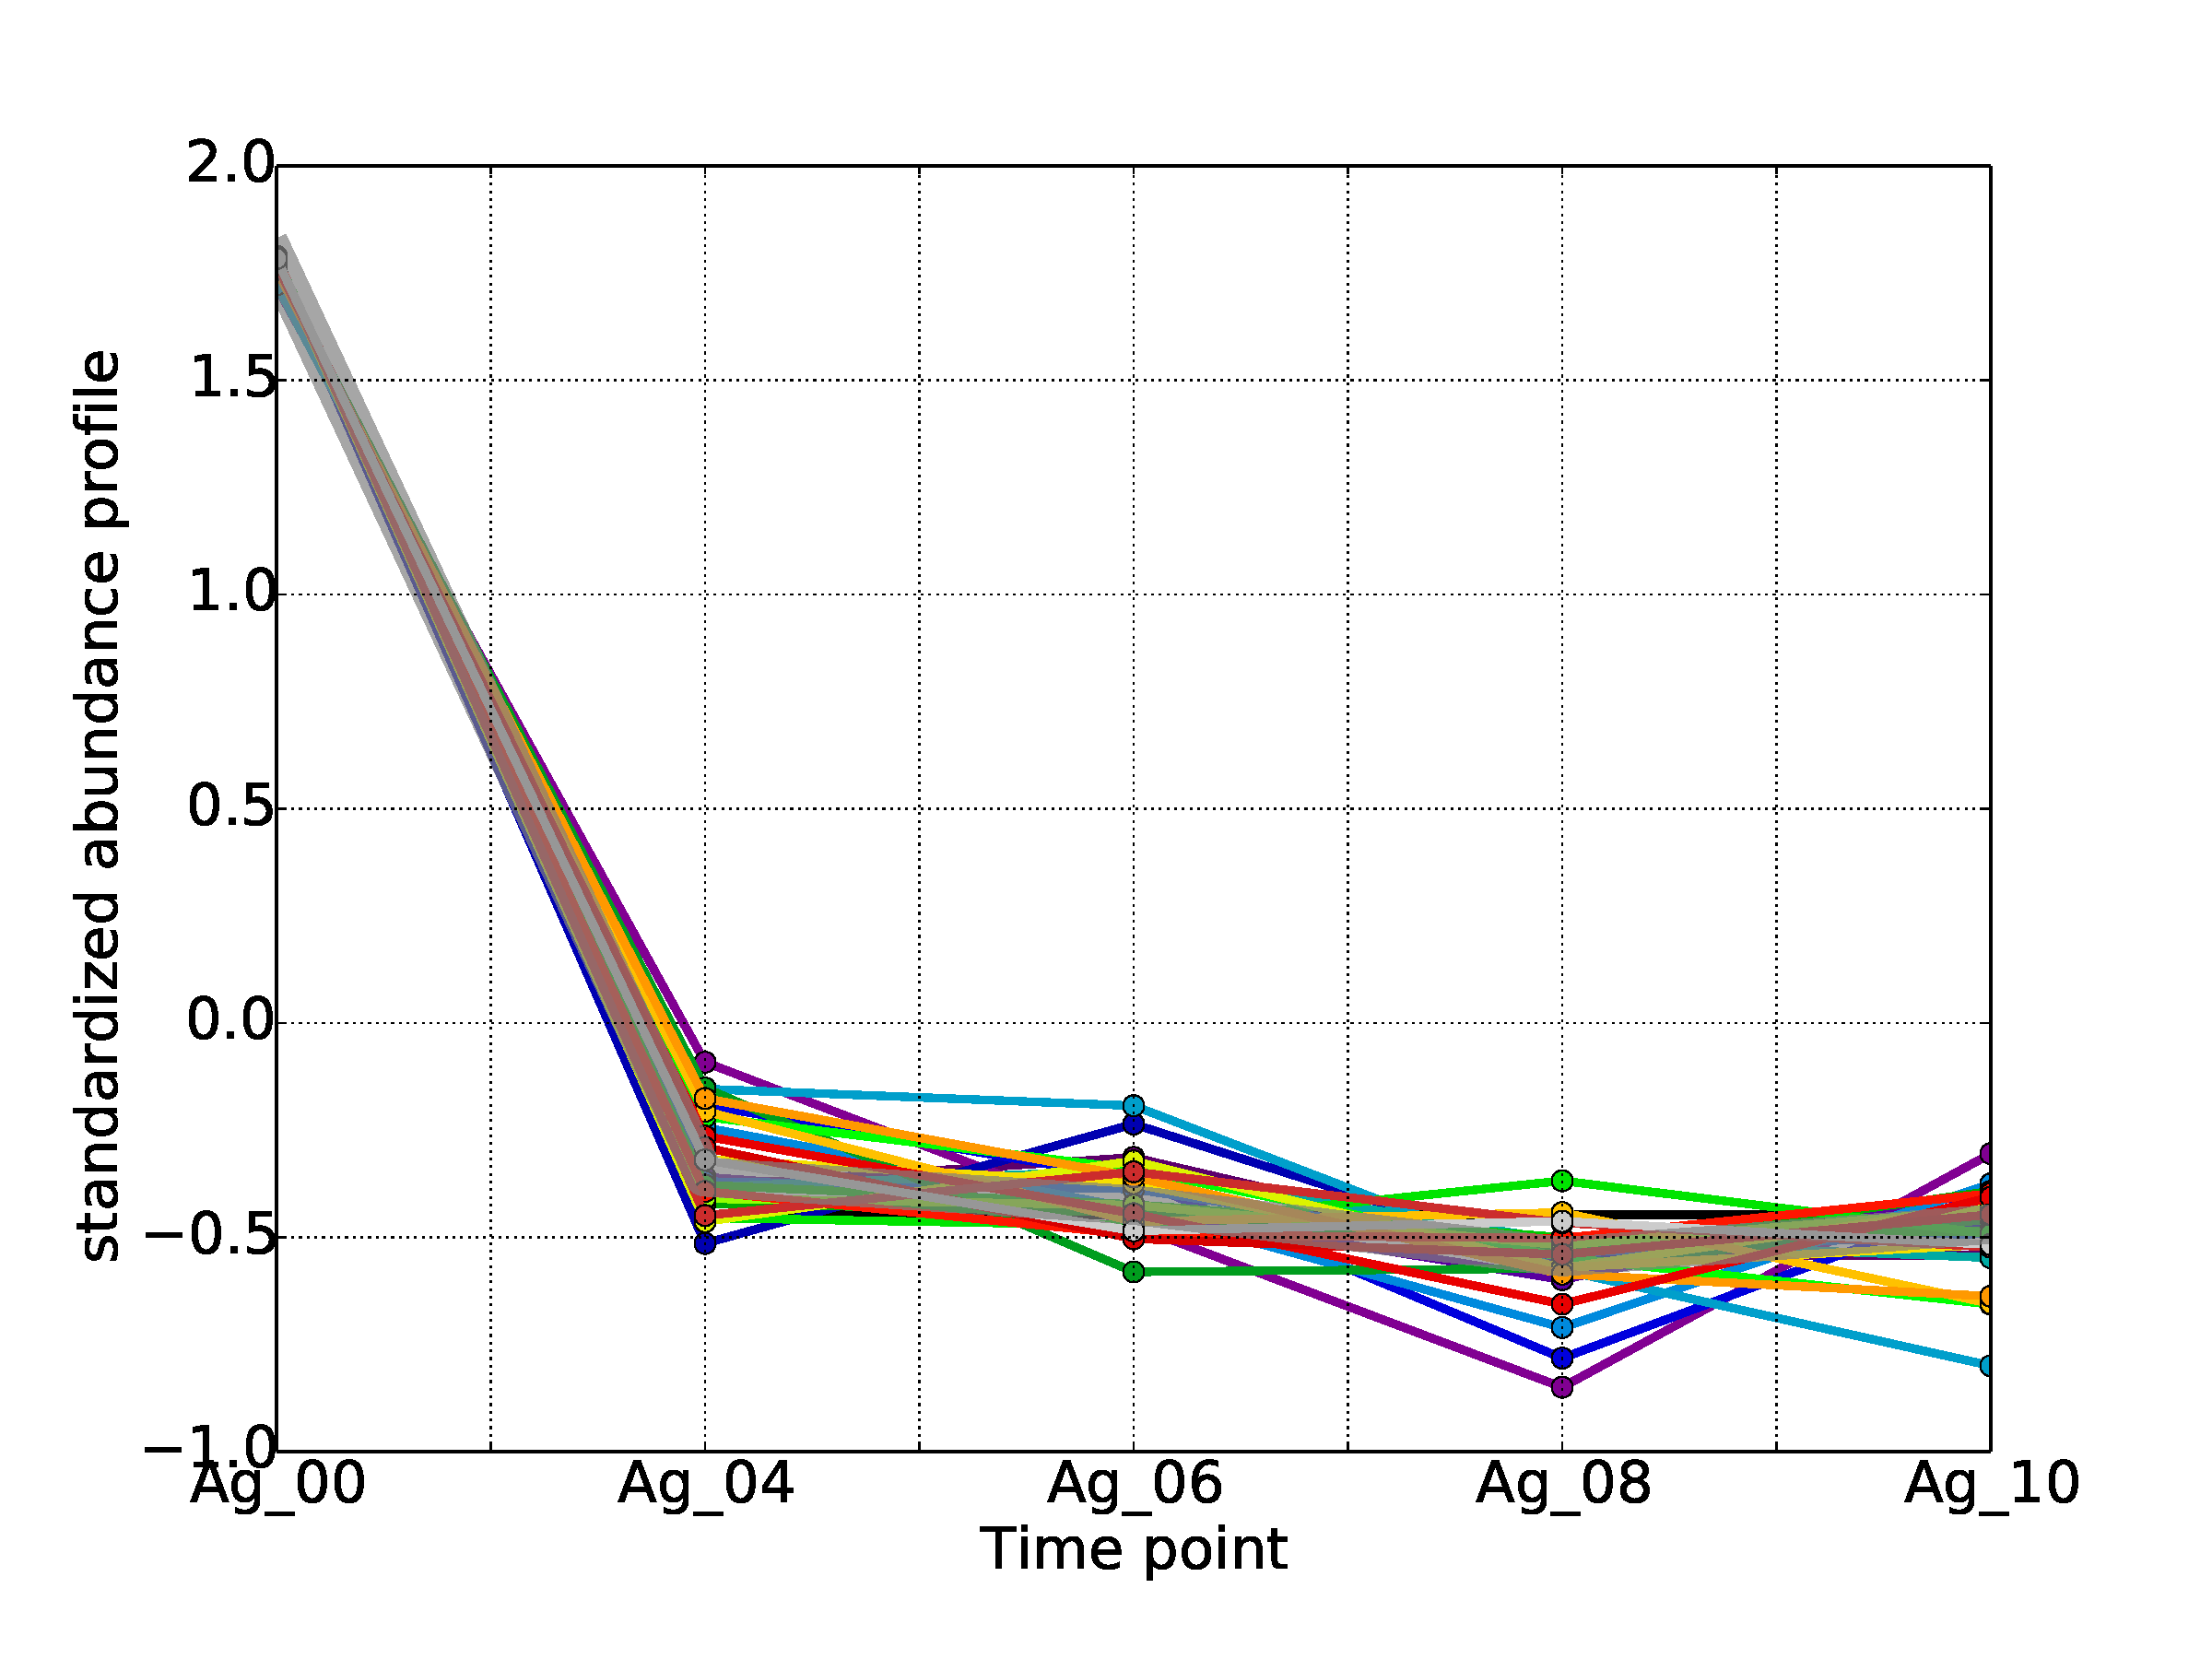
\includegraphics[width=.5\linewidth]{figures/figs/ecr_and_insects_ptci_20130918_orthodb7/downAfter4_gene_profiles_from_cummerbund/Ag_downAfter4_cls6_Ag_target_FPKMs_vb_orthos.pdf}}
%
\subcaptionbox{\label{fig:cluster6-Cq}}
{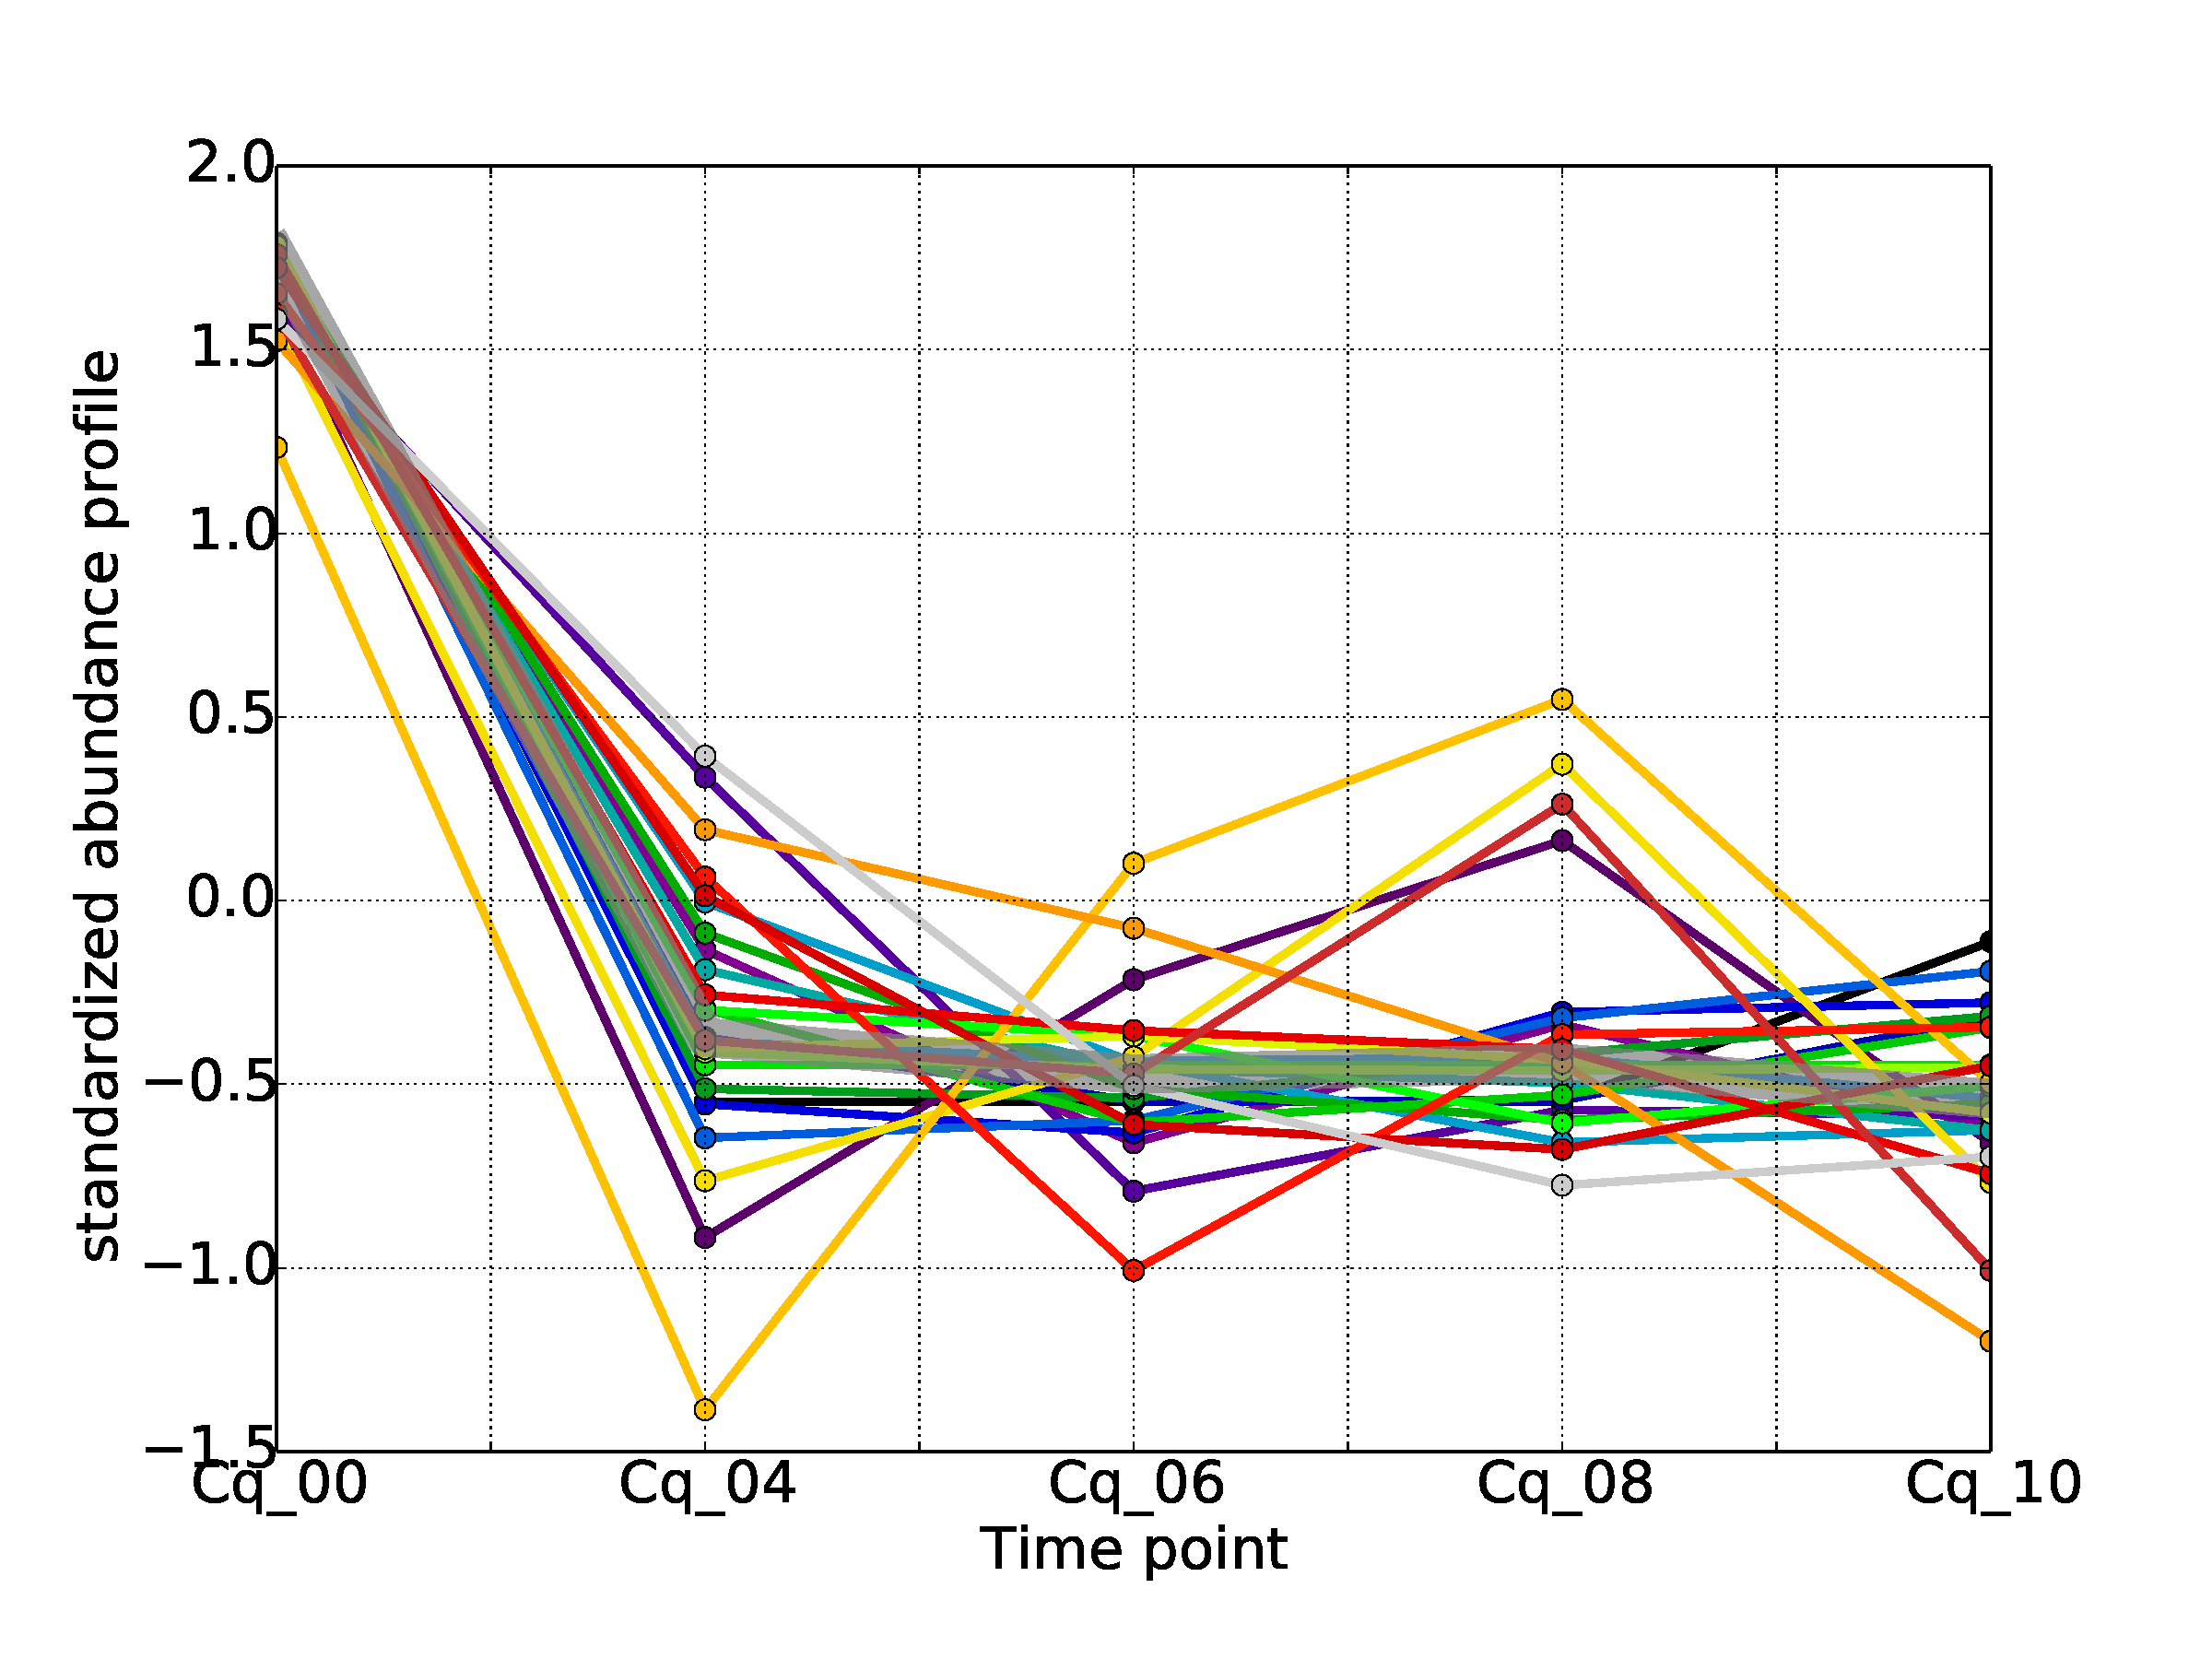
\includegraphics[width=.5\linewidth]{figures/figs/ecr_and_insects_ptci_20130918_orthodb7/downAfter4_gene_profiles_from_cummerbund/Cq_downAfter4_cls6_Ag_target_FPKMs_vb_orthos.pdf}}
% 
\caption[Orthologs of cluster 6]{\sf \textbf{Orthologs of cluster 6 (down after 4h):}\\
The same color scheme is used for each species which means that orthologs are given the same color in all three panels.
The thick, transparent gray line represents the median \gls{mAP} for the panel.
\textbf{(A)} \Aa.
\textbf{(B)} \Ag.
\textbf{(C)} \Cq.
}\label{fig:cluster6}
\end{figure}
% Figure \ref{fig:cluster6}
% 
% 
\begin{figure}[hp]
% 
\begin{subfigure}[t]{.5\linewidth}
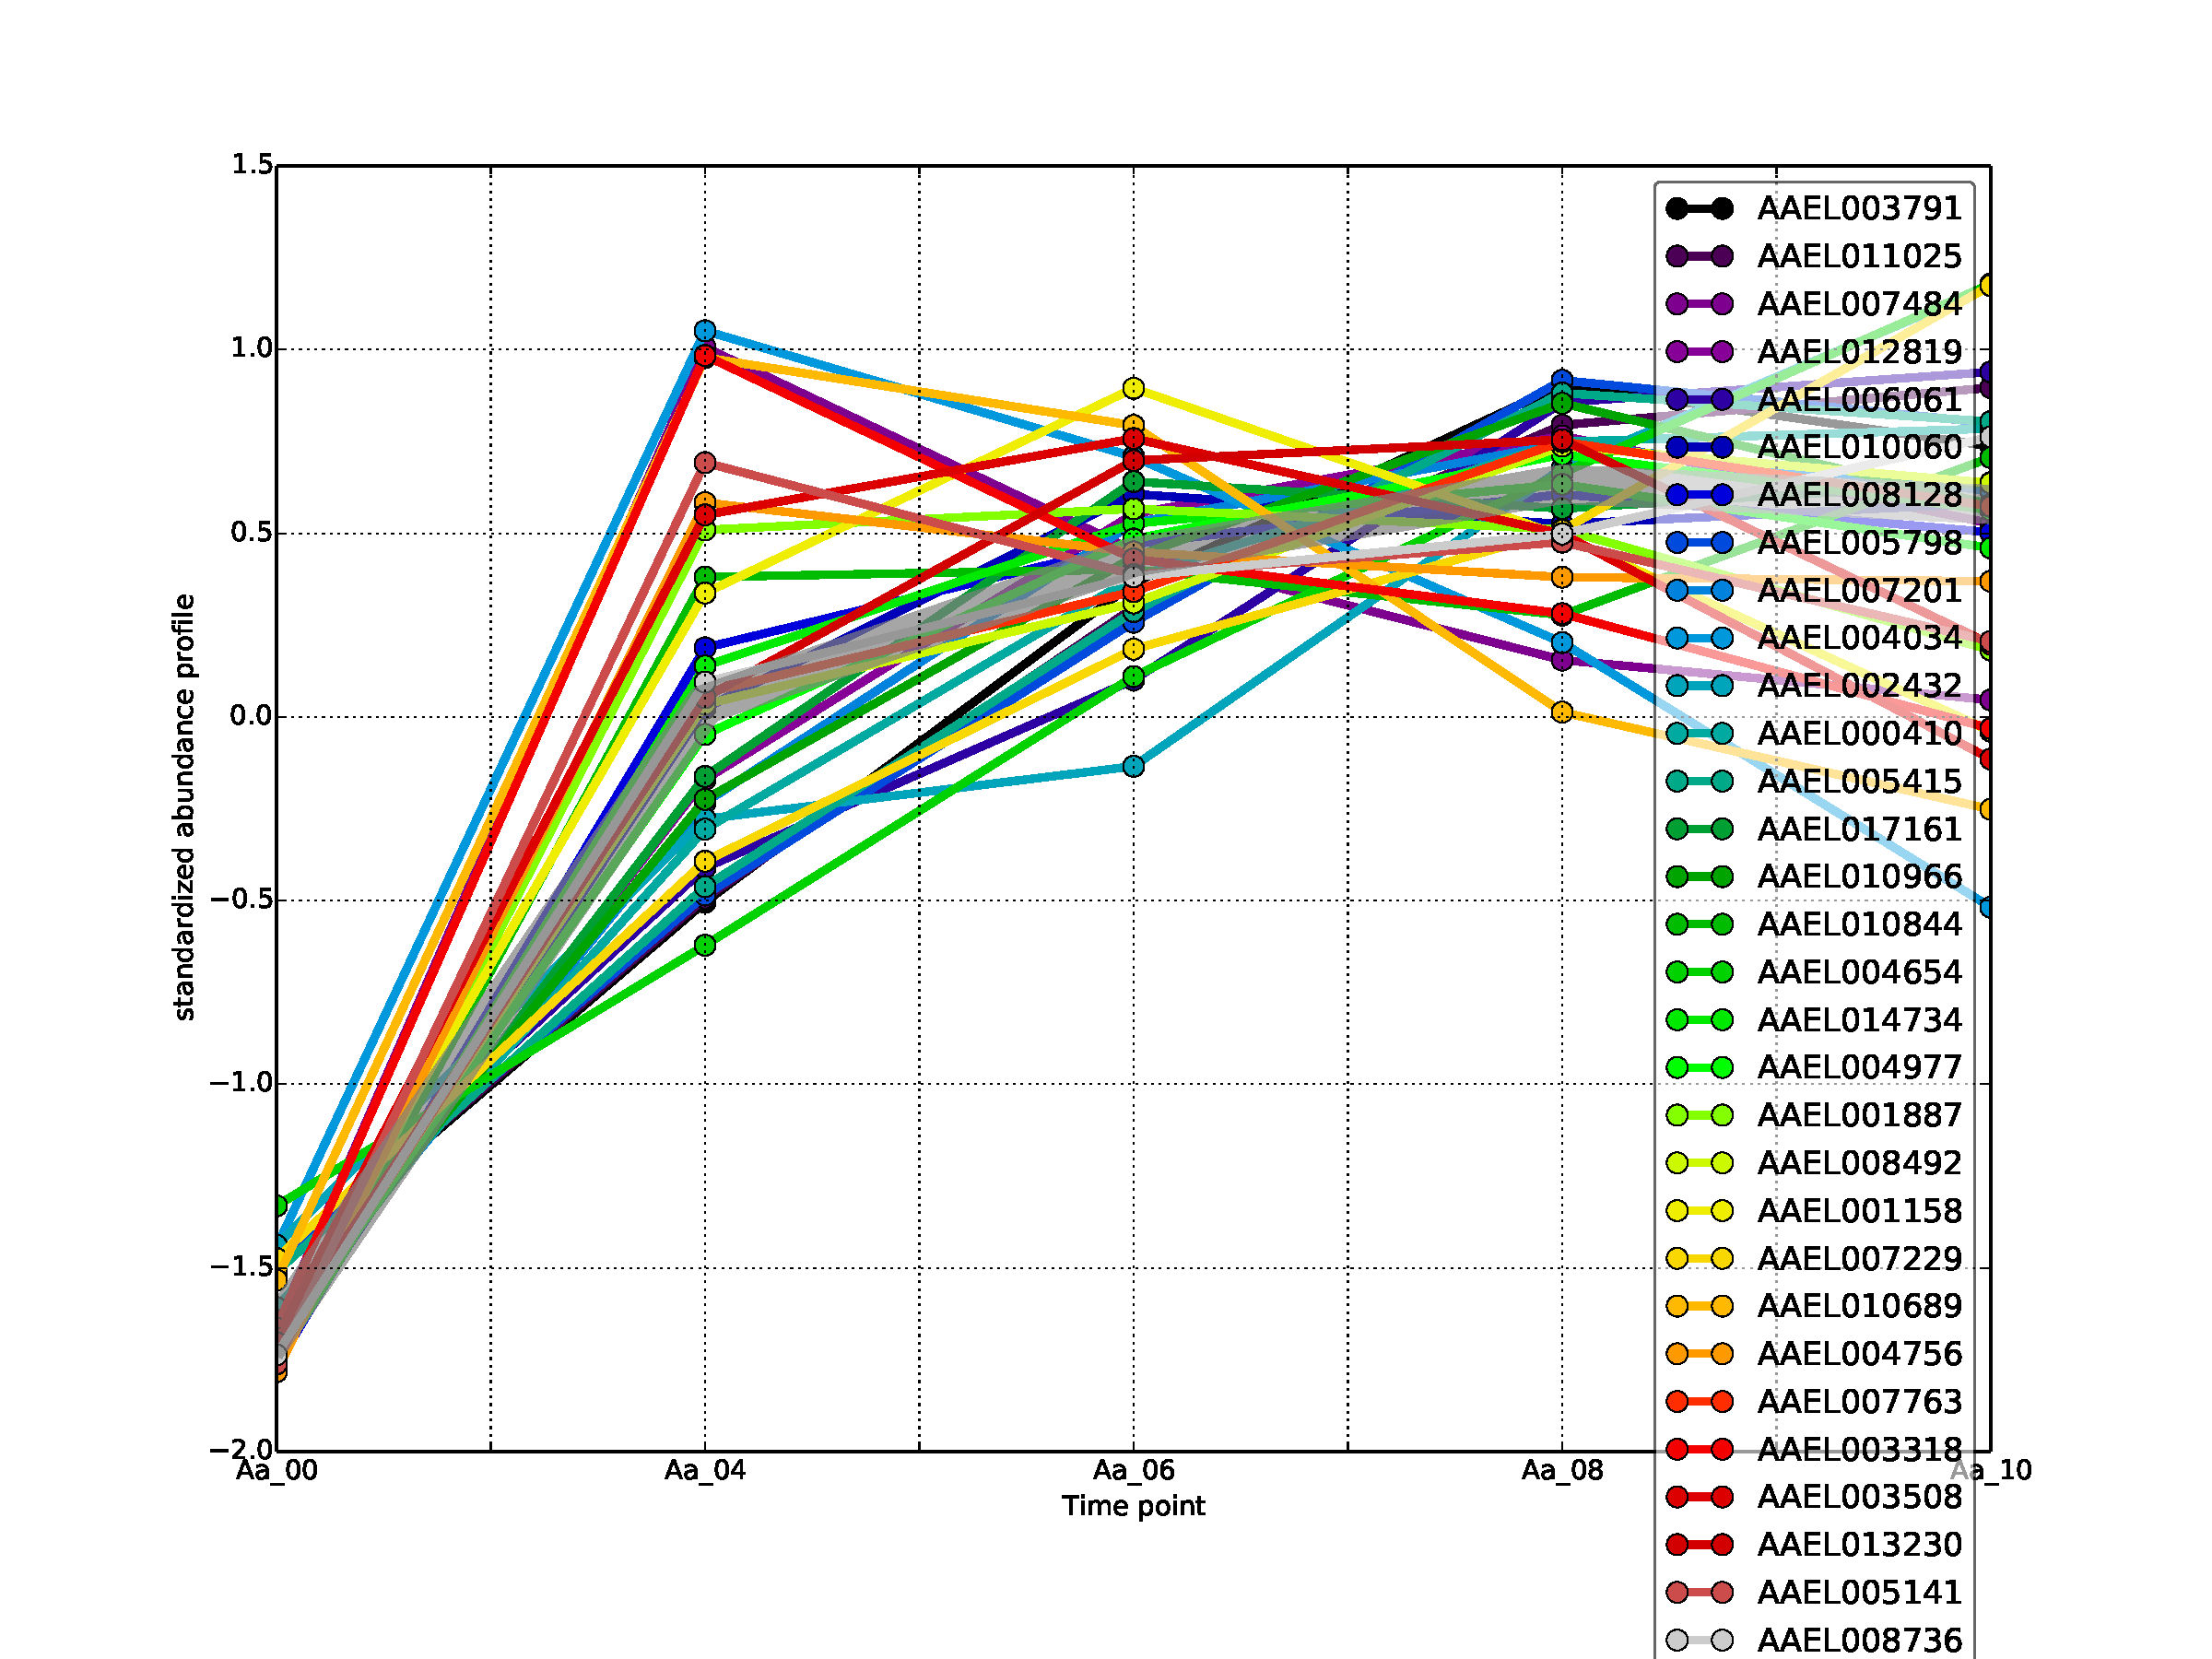
\includegraphics[width=\linewidth]{figures/figs/ecr_and_insects_ptci_20130903/upAfter4_gene_profiles_from_cummerbund/Aa_upAfter4_cls7_Ag_target_FPKMs_vb_orthos.pdf}
\caption{}
\label{fig:cluster7-Aa}
\end{subfigure}%
%
\begin{subfigure}[t]{.5\linewidth}
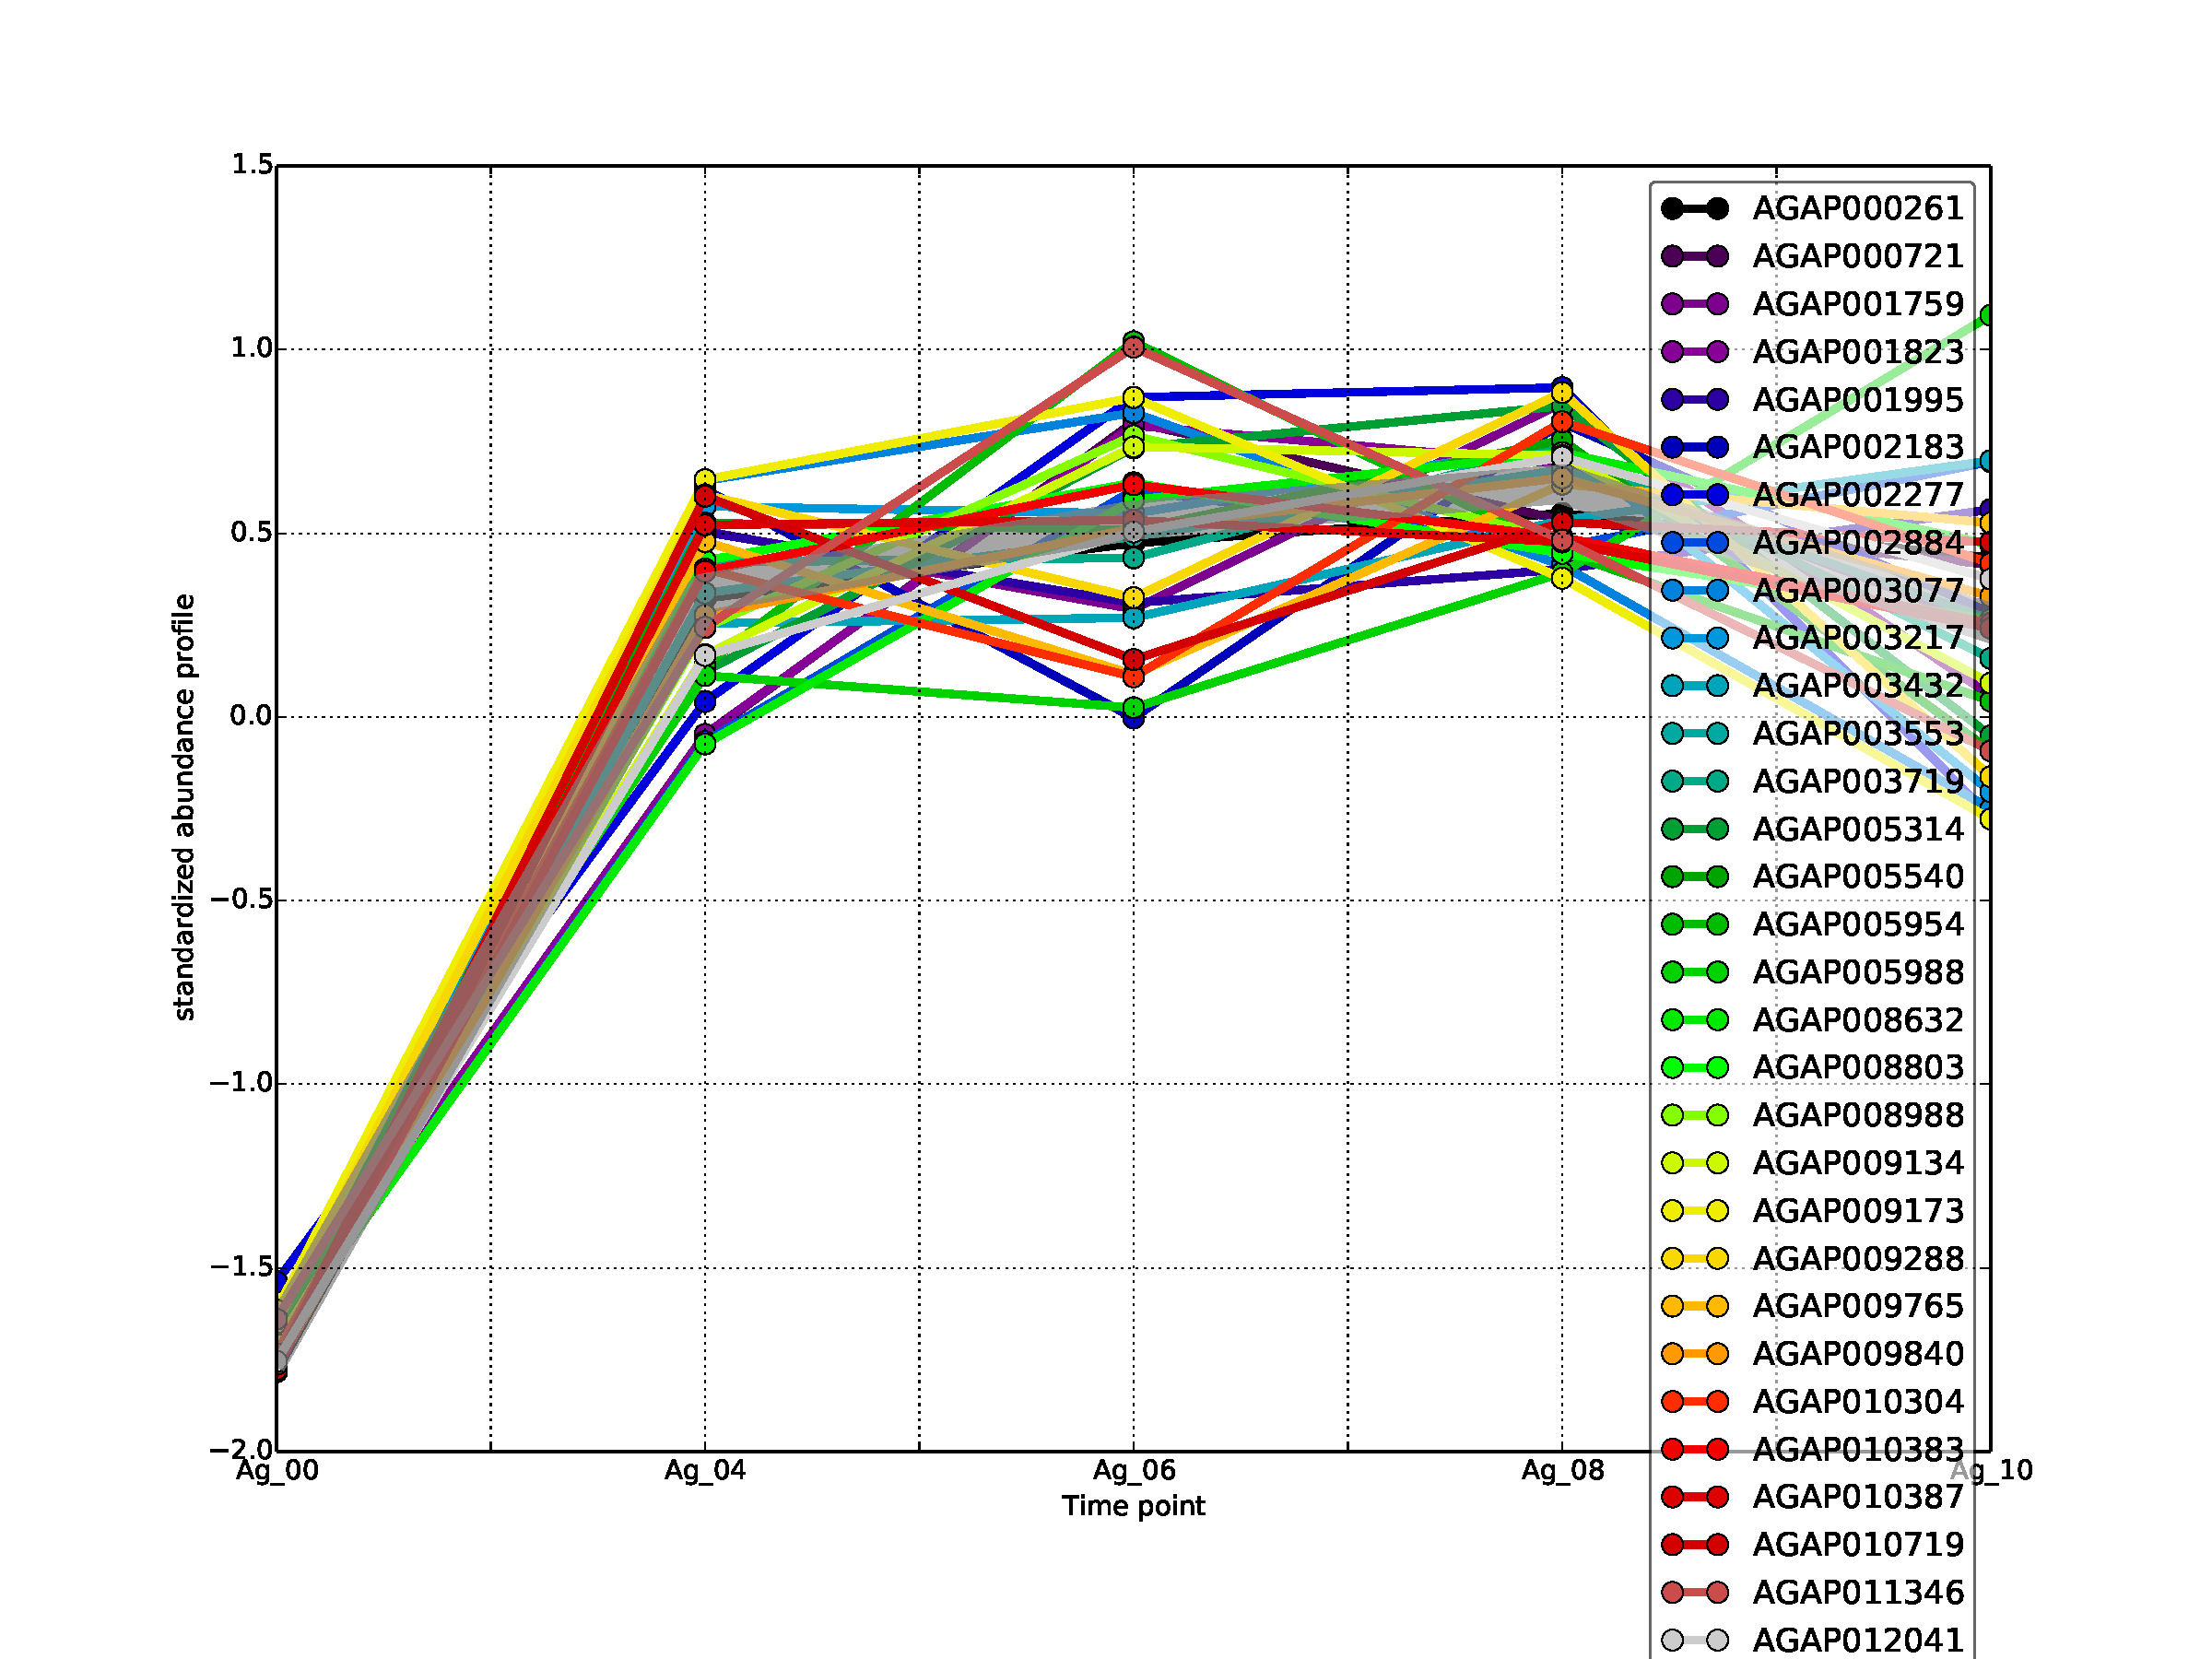
\includegraphics[width=\linewidth]{figures/figs/ecr_and_insects_ptci_20130903/upAfter4_gene_profiles_from_cummerbund/Ag_upAfter4_cls7_Ag_target_FPKMs_vb_orthos.pdf}
\caption{}
\label{fig:cluster7-Ag}
\end{subfigure}
% 
\begin{subfigure}[t]{.5\linewidth}
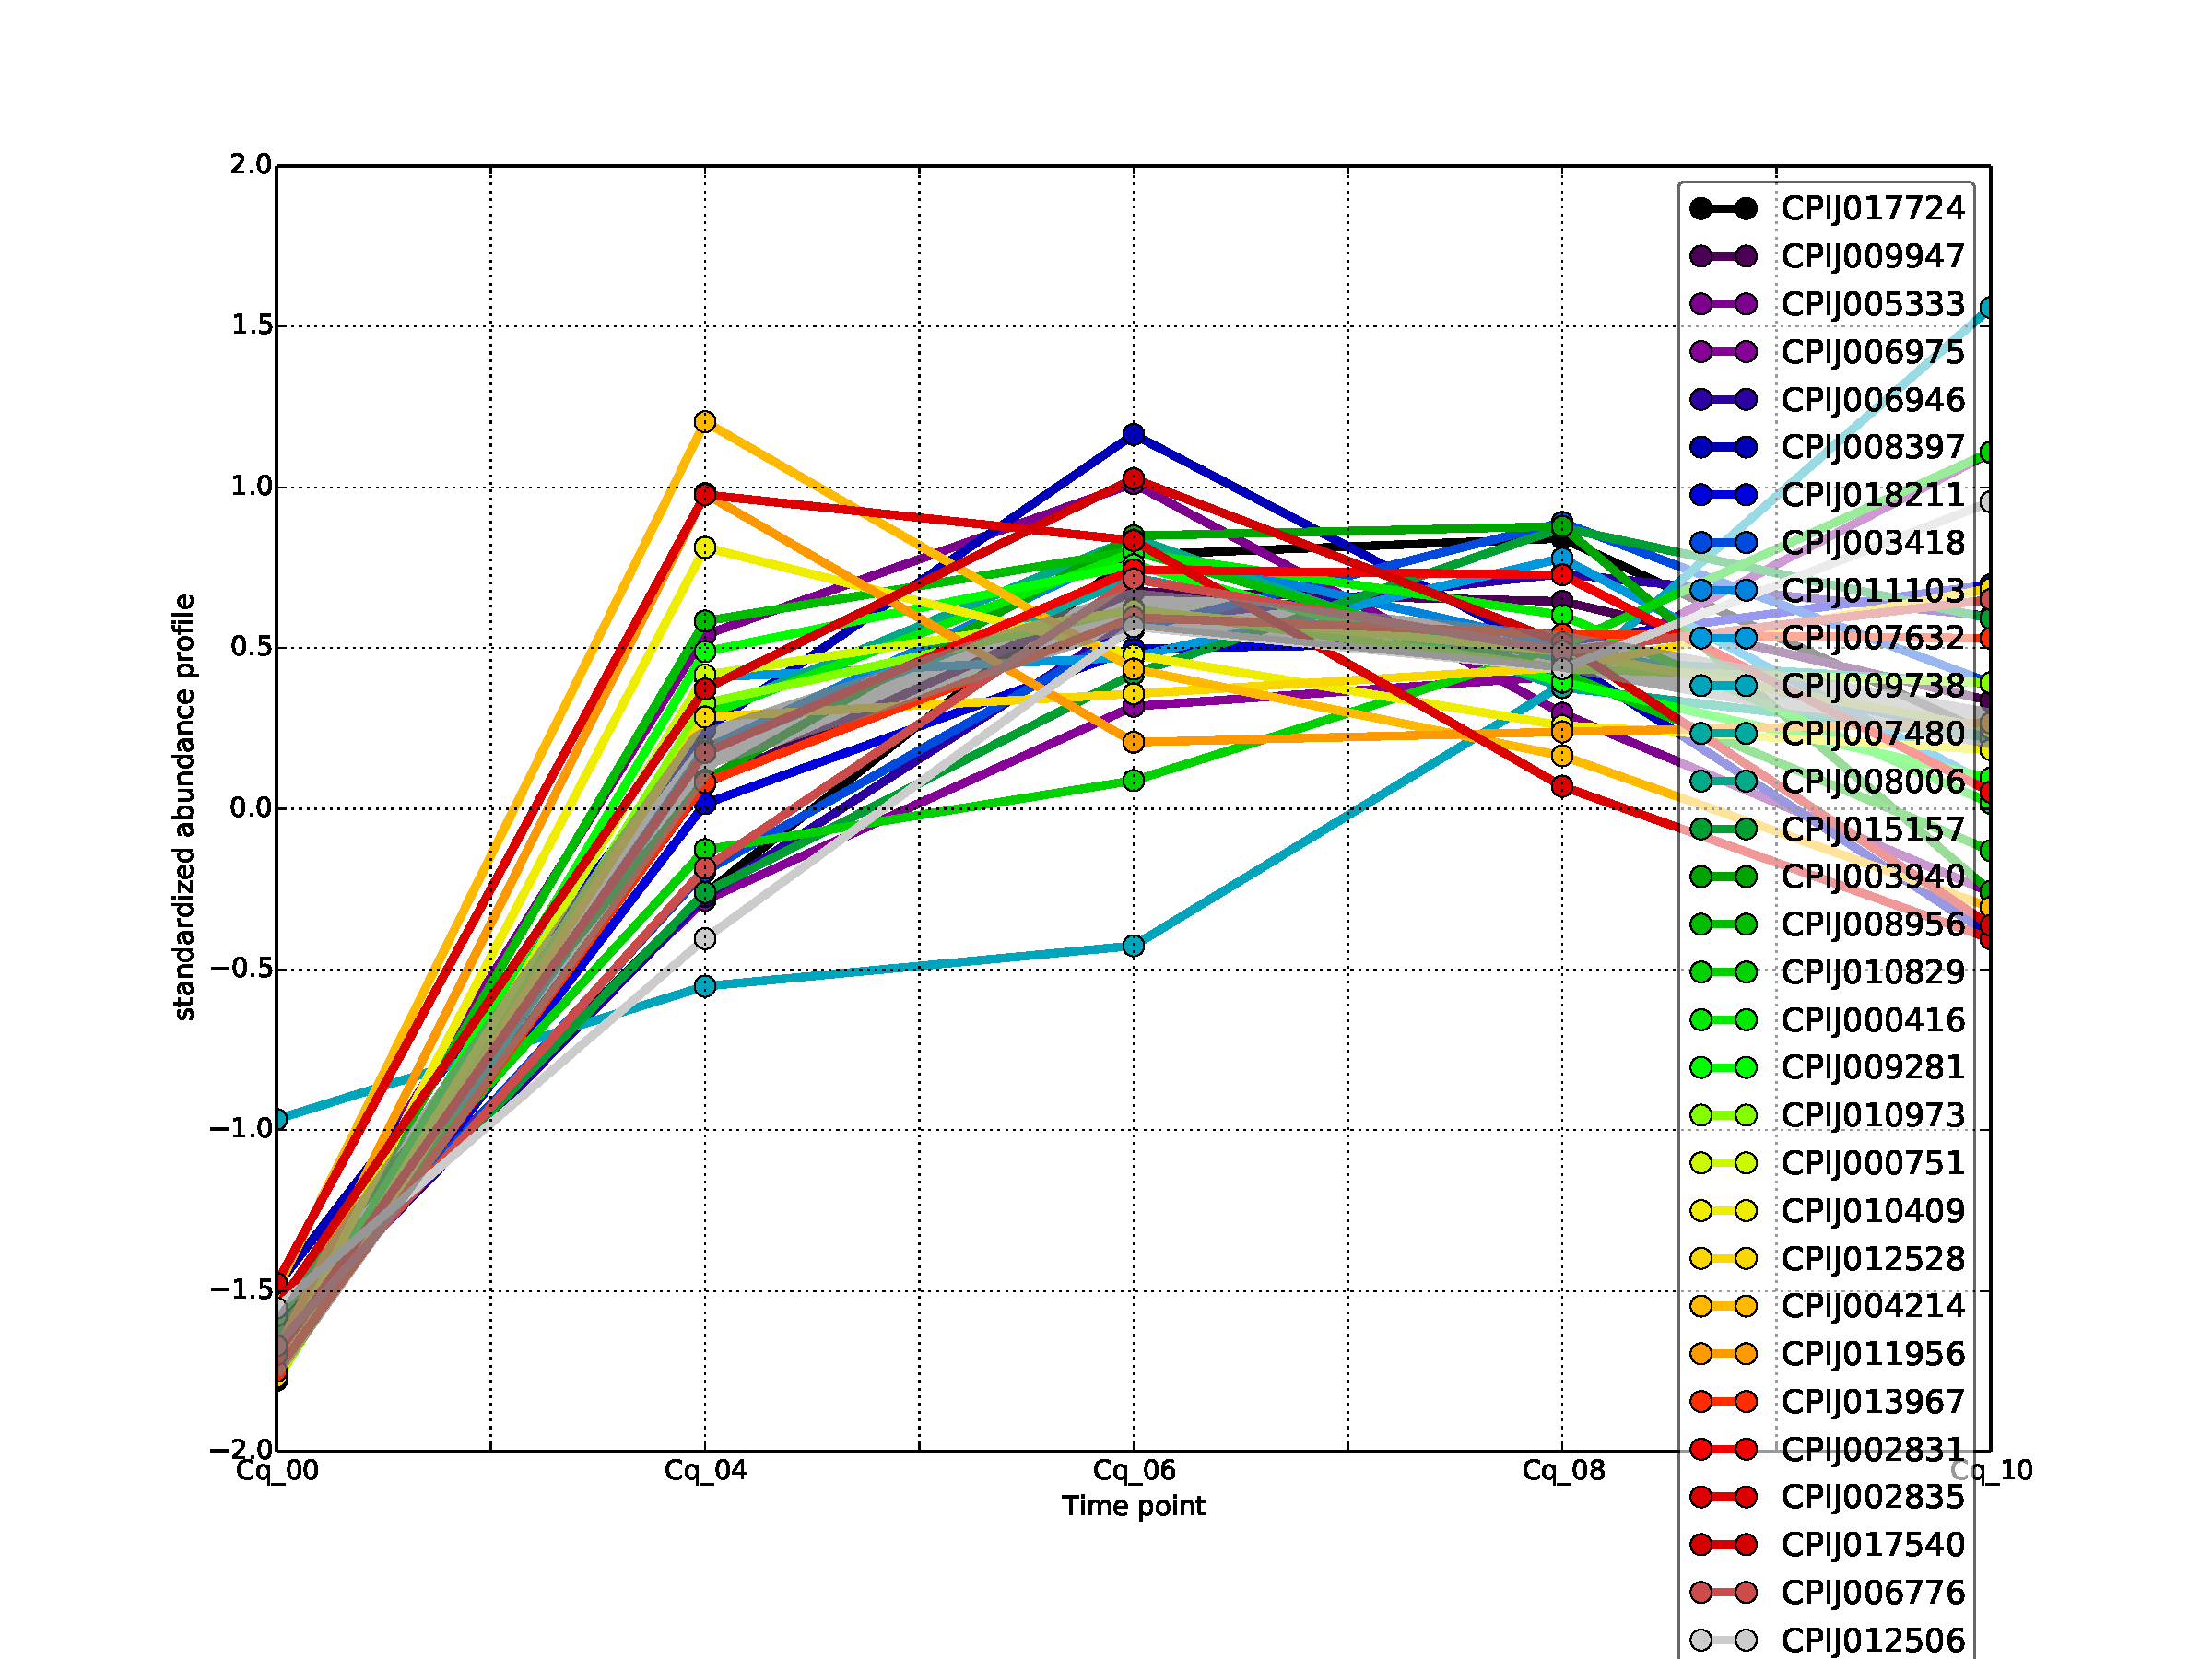
\includegraphics[width=\linewidth]{figures/figs/ecr_and_insects_ptci_20130903/upAfter4_gene_profiles_from_cummerbund/Cq_upAfter4_cls7_Ag_target_FPKMs_vb_orthos.pdf}
\caption{}
\label{fig:cluster7-Cq}
\end{subfigure}
% 
\caption[Orthologs of cluster 7]{\sf \textbf{Orthologs of cluster 7:}\\

\textbf{(A)} \Aa.
\textbf{(B)} \Ag.
\textbf{(C)} \Cq.
\todo[inline,caption={Finish Fig \ref{fig:cluster7}}]{ 
\begin{itemize}
    \item the text
    \item double gene names
    \item fix fig widths
\end{itemize}}
}
\label{fig:cluster7}
\end{figure}
% Figure \ref{fig:cluster7}
% 
% \input{/home/gus/Dropbox/common/projects/Aa_Ag_Cq_As/gfunc_stuff/prelim_gene_analysis/ecr_OR_insect_20130903/ptci_1_0/clusters/cls7/pandas_out/process.tex}
% Table \ref{tab:cluster7-P-mean-TS}
% 
% 
% 
\begin{figure}[hp]
% 
\begin{subfigure}[t]{.5\linewidth}
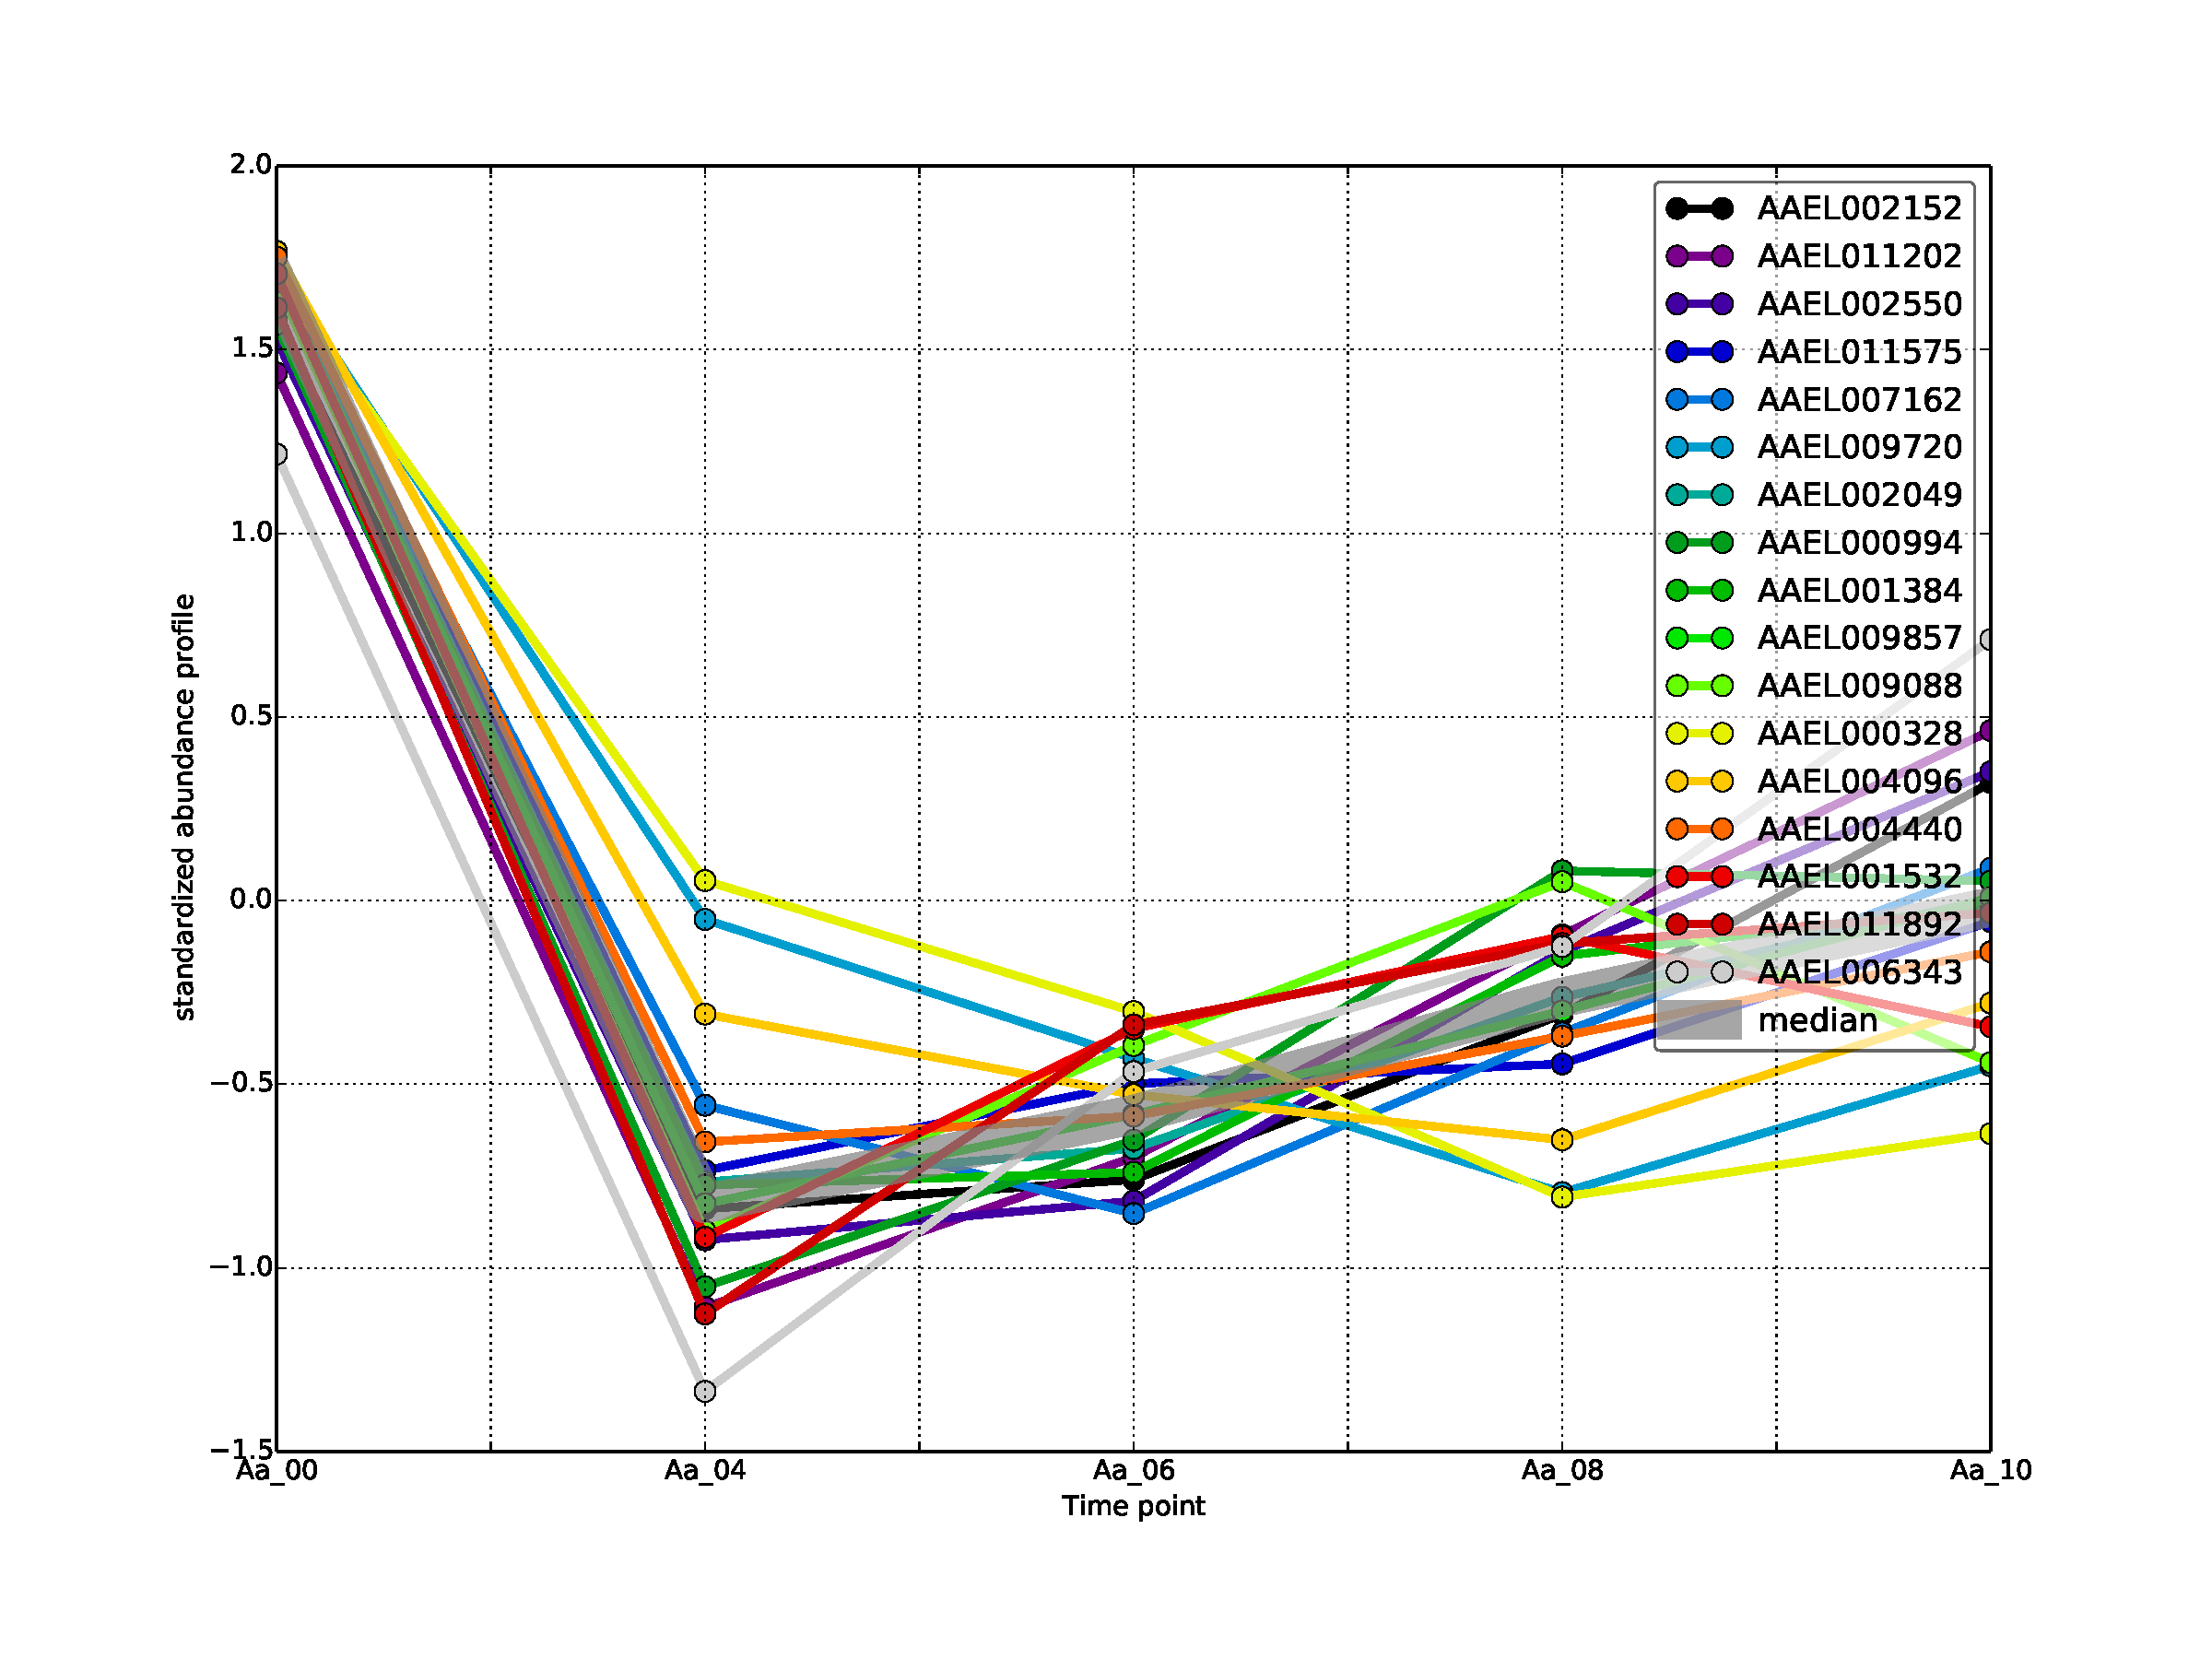
\includegraphics[width=\linewidth]{figures/figs/ecr_and_insects_ptci_20130903/downAt4_gene_profiles_from_cummerbund/Aa_downAt4_cls19_Ag_target_FPKMs_vb_orthos.pdf}
\caption{}
\label{fig:cluster19-Aa}
\end{subfigure}%
%
\begin{subfigure}[t]{.5\linewidth}
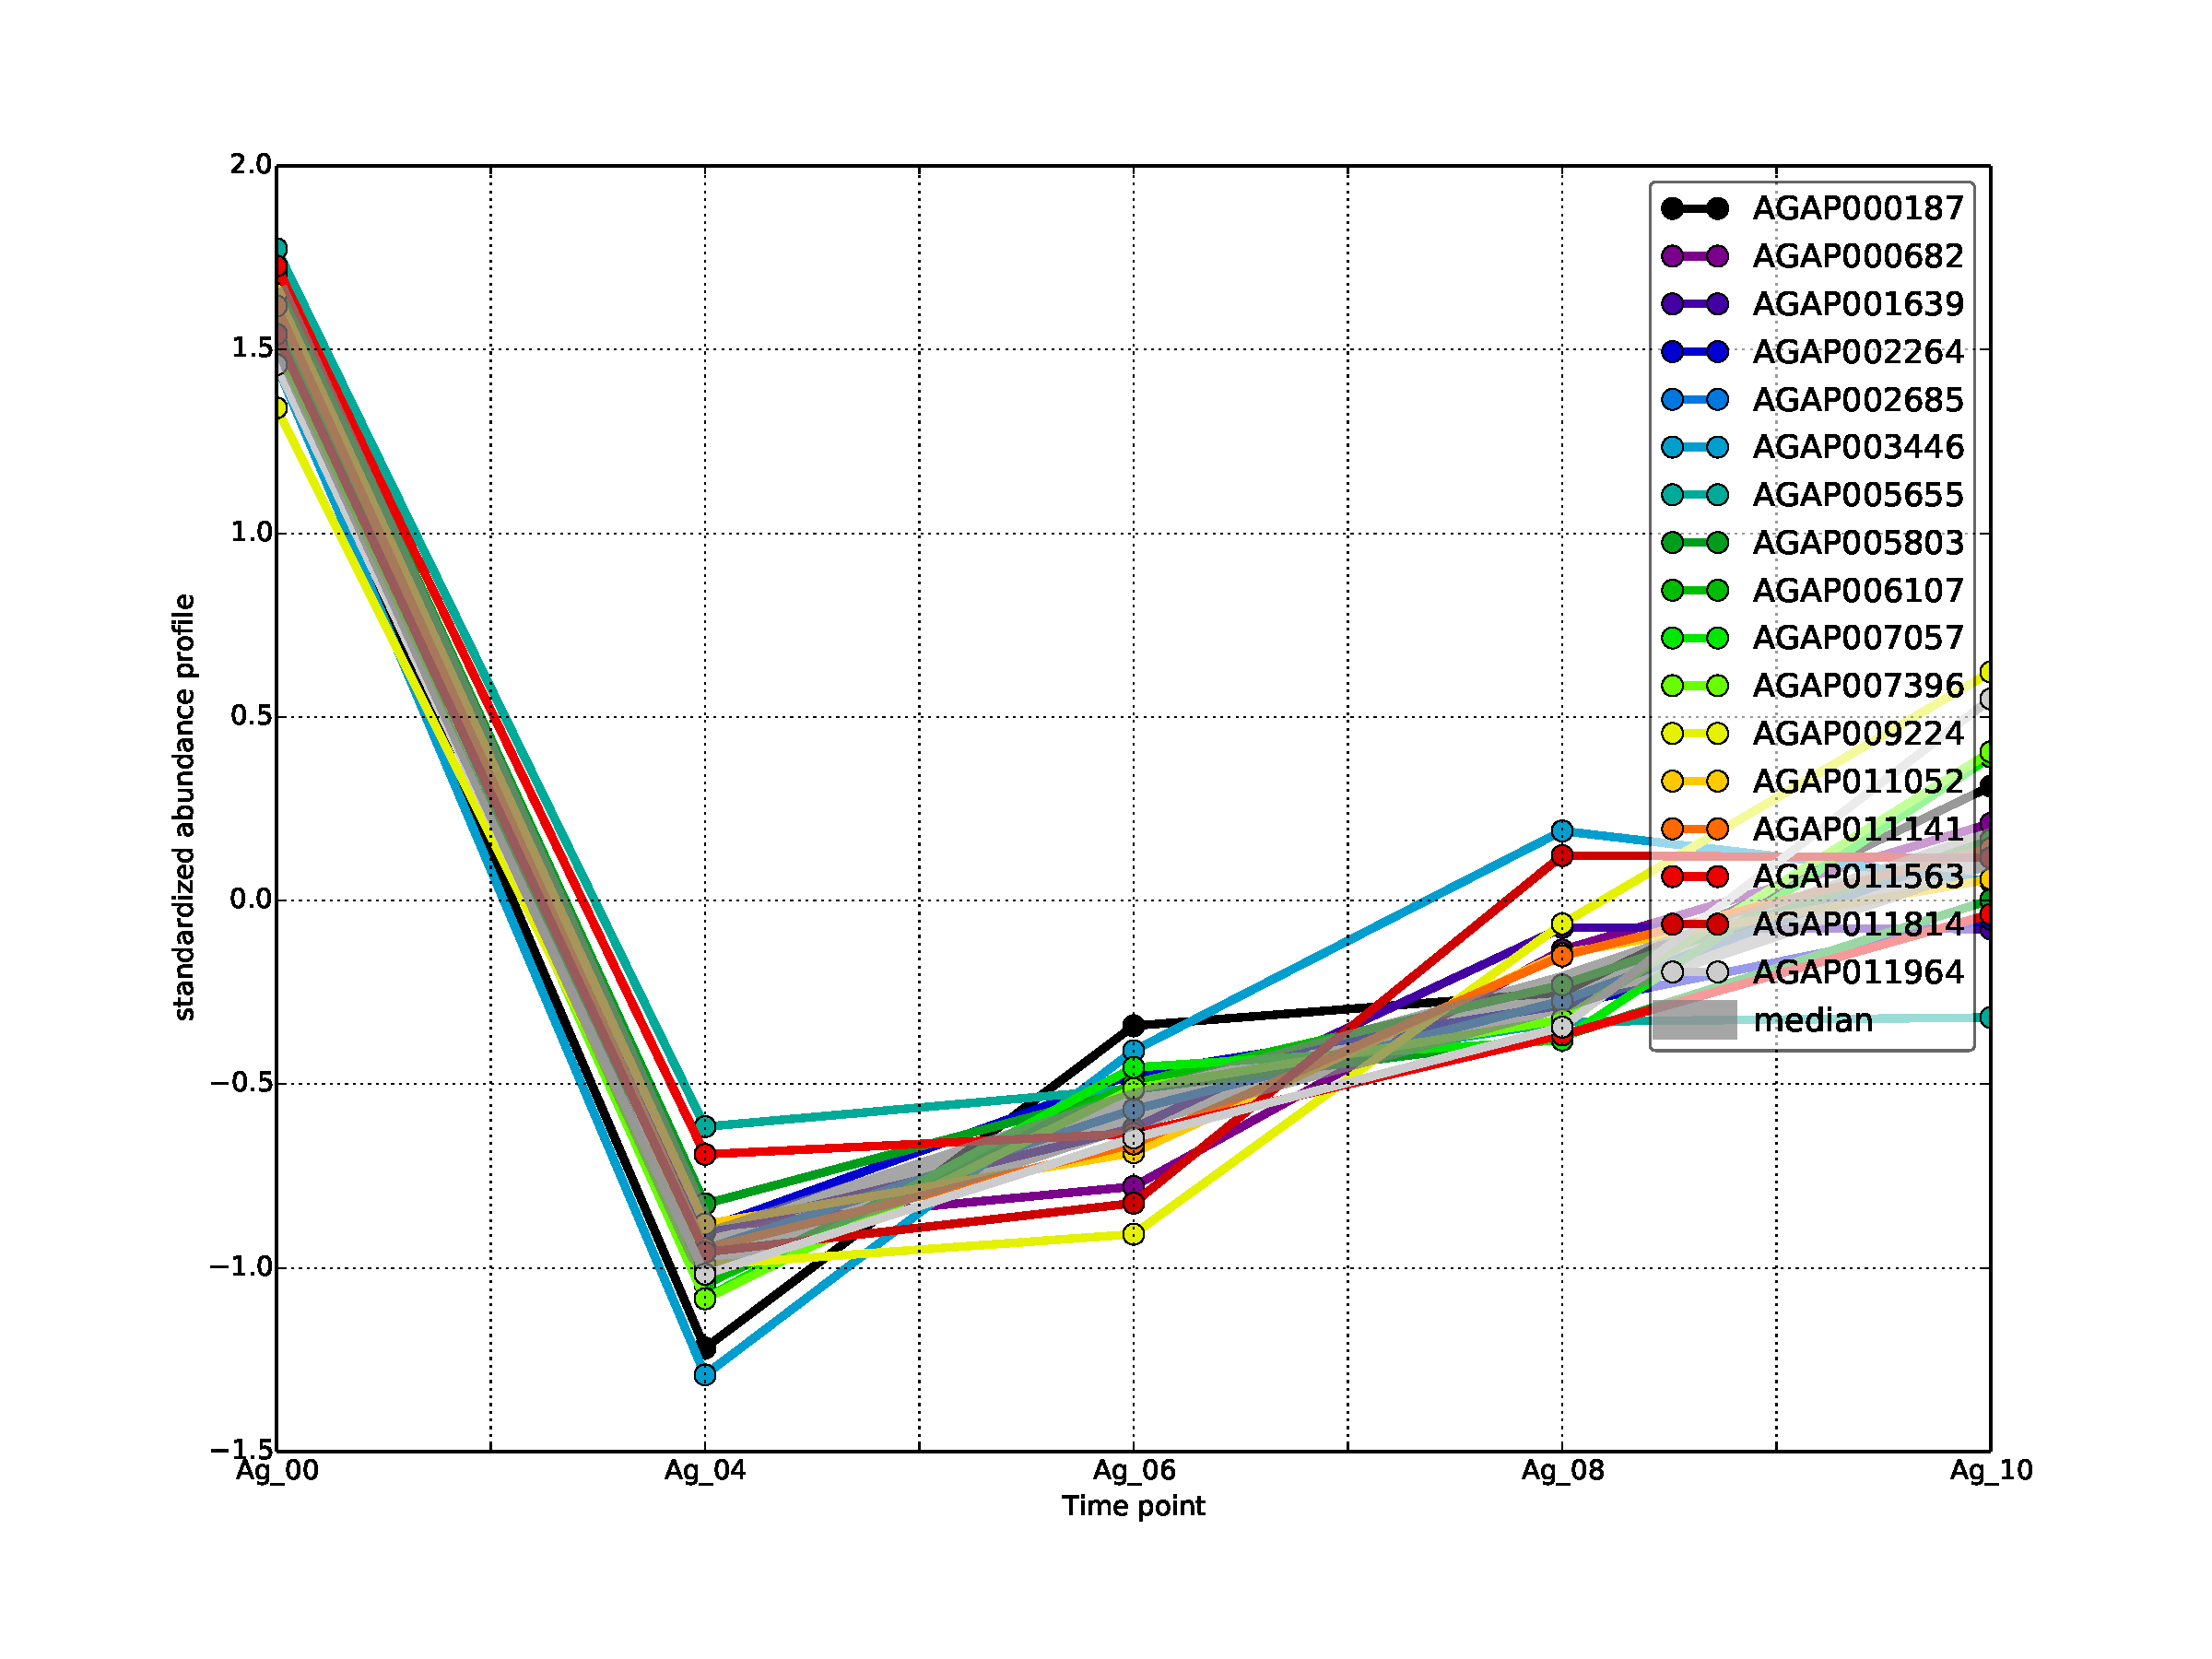
\includegraphics[width=\linewidth]{figures/figs/ecr_and_insects_ptci_20130903/downAt4_gene_profiles_from_cummerbund/Ag_downAt4_cls19_Ag_target_FPKMs_vb_orthos.pdf}
\caption{}
\label{fig:cluster19-Ag}
\end{subfigure}
% 
\begin{subfigure}[t]{.5\linewidth}
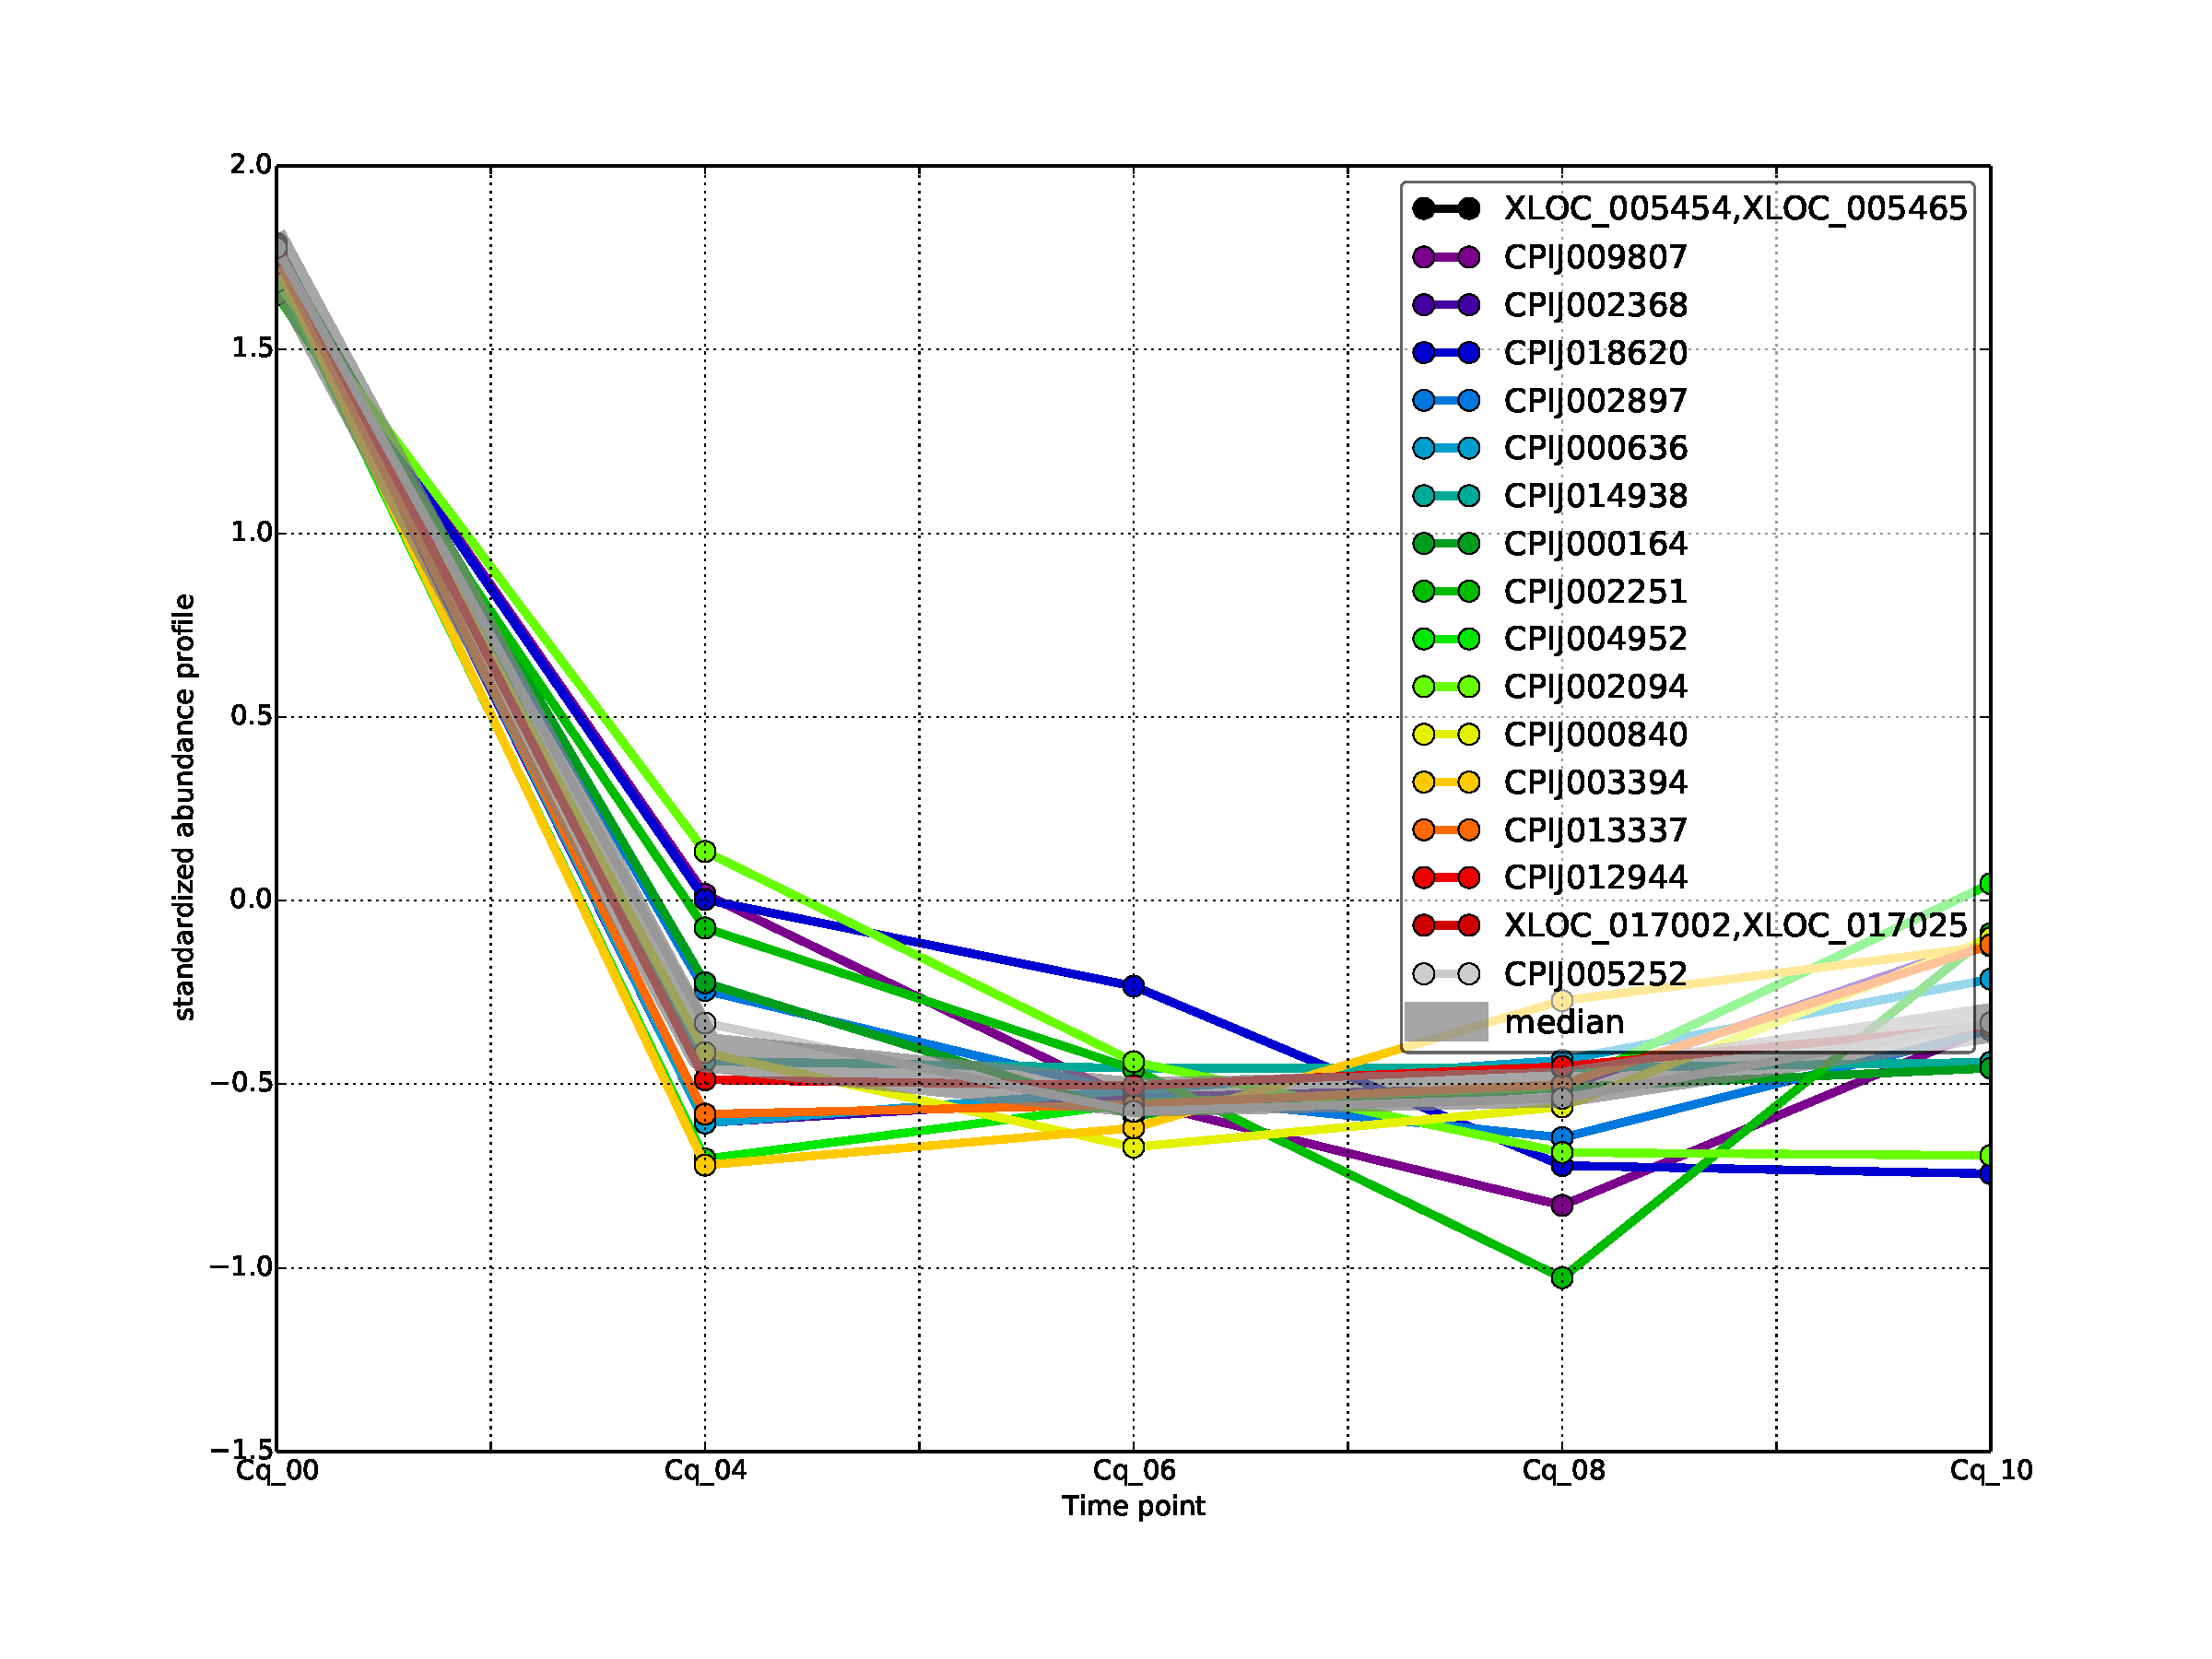
\includegraphics[width=\linewidth]{figures/figs/ecr_and_insects_ptci_20130903/downAt4_gene_profiles_from_cummerbund/Cq_downAt4_cls19_Ag_target_FPKMs_vb_orthos.pdf}
\caption{}
\label{fig:cluster19-Cq}
\end{subfigure}
% 
\caption[Orthologs of cluster 19]{\sf \textbf{Orthologs of cluster 19:}\\

\textbf{(A)} \Aa.
\textbf{(B)} \Ag.
\textbf{(C)} \Cq.
\todo[inline,caption={Finish Fig \ref{fig:cluster19}}]{Finish this fig: 
\begin{itemize}
    \item the text
    \item double gene names
    \item fix fig widths
\end{itemize}}
}
\label{fig:cluster19}
\end{figure}
% Figure \ref{fig:cluster19}



%%% Local Variables: ***
%%% mode: latex ***
%%% TeX-master: "thesis.tex" ***
%%% End: ***

\chapter{Contributions to Literature Not Otherwise Mentioned}
\todo[inline]{decide whether this gets included}
\section{Purpose}
xxxxxxxxxxxxxxxxxxxxxxxxxx
\begin{enumerate}
 \item xxx
\end{enumerate}


%%% Local Variables: ***
%%% mode: latex ***
%%% TeX-master: "thesis.tex" ***
%%% End: ***

\chapter{Conclusions}

\section{Purpose}
xxxxxxxxxxxxxxxxxxxxxxxxxx
\begin{enumerate}
 \item xxx
\end{enumerate}

%%% Local Variables: ***
%%% mode: latex ***
%%% TeX-master: "thesis.tex" ***
%%% End: ***



% ... and so on

% These commands fix an odd problem in which the bibliography line
% of the Table of Contents shows the wrong page number.
\clearpage
\phantomsection

% "References should be formatted in style most common in discipline",
% abbrv is only a suggestion.
\bibliographystyle{abbrv}
\bibliography{thesis}

% The Thesis Manual says not to include appendix figures and tables in
% the List of Figures and Tables, respectively, so these commands from
% the caption package turn it off from this point onwards. If needed,
% it can be re-enabled later (using list=yes argument).
\captionsetup[figure]{list=no}
\captionsetup[table]{list=no}

% If you have an appendix, it should come after the references.
% The original template (from Trevor) had a custom \appendix command,
% but I found it to break figure/table counters. I'm not sure how
% reliable my fix is, so I ended up reverting back to the standard
% latex version, and renaming the custom command to \myappendix.  You
% can try both and see how things work out:
% 1) Call \appendix once, and then make each appendix a \chapter
% 2) Call \myappendix once, and then make each appendix a \section.

\appendix

\printglossaries

\chapter{Methods}

\section{Comparative genomics allows the discovery of \textit{cis}-regulatory elements in mosquitoes}
% CITEME 3  Nene2007
% CITEME 13 Marinotti2005
% CITEME 14 Marinotti2006
% CITEME 50 Vilella2009
% CITEME 51 Richardson2006
% CITEME 52 Mahony2007stamp
% CITEME 53 Mahony2007dna
% CITEME 54 Benjamini1995
% CITEME 55 Saeed2003

\subsection{Sequence Datasets}
Orthologous gene pairs among \Cxq\ (genebuild CpiJ1.2), \Aea\ (genebuild AaegL1.1), \Ang\ (genebuild AgamP3.4), and \Dmel\ (genebuild BDGP4.3) were determined using the Ensemble Compara pipeline \cite{Vilella2009}.
This pipeline is based on maximum likelihood phylogenetic gene trees built from the gene transcripts and representing the evolutionary history of gene families.
Duplication or speciation events are differentiated by comparing the gene trees to the species tree.
This method is analogous to the reciprocal best-hit approach in the simple case of unique orthologous genes (one-to-one orthologues).
The resulting lists of genes are available from Vectorbase at \url{http://www.vectorbase.org/Other/ComparativeAnalyses}.
All mosquito gene coordinates were obtained from VectorBase and \Dm\ data were from Ensembl API (\Aa: Ensembl 49 genebuild AaeL1.1; \Ag: Ensembl 49, genebuild Agam3.4; \Cq: VectorBase, genebuild CpiJ1.2; \Dm: Ensemble 49, genebuild BDGP4.3).
Repeat-masked \Cq\ sequences were obtained from VectorBase and all other genome sequences were retrieved premasked using the Ensembl perl API.
The one-to-one mosquito orthologous datasets were evaluated further before using in the MDOS analyses.
The pronounced intron elongation in 5′- and 3′-end UTRs resulting from the insertion of repetitive elements within these regions \cite{Nene2007} and the presence of coding sequence incorrectly included in annotated UTRs were mitigated by only using sequences found within fragments 2 kb in length at the 5′-end of the annotated gene boundaries.
Overlaps of these DNA sequences with adjacent genes were determined through use of fjoin \cite{Richardson2006} and the sequences truncated accordingly.
Only sequences with a final size ≥ 10 base (bp) were analyzed.
Pairwise comparisons were conducted with MDOS limits set for the discovery of 7-, 8-, and 9-mers.

\subsection{Discovery of Evolutionarily Conserved Putative CREs Among Mosquitoes}
Motifs receiving a conservation z-score ≥3 in all 3 mosquito pairwise comparisons were combined into a nonredundant list.
To discover motifs with greater exclusivity within the 3 mosquitoes, the conservation z-scores for each motif in 2-kb 5′-end flanking regions of shared \Dm\ orthologues also were determined.
A reciprocal analysis was conducted in which 8-mers conserved in 5′-end flanking regions of one-to-one orthologs of \Dm\ and each mosquito species also were determined (conservation z-score ≥3), followed by conservation z-scores determination of these motifs in the other 2 mosquito species.
This analysis addresses the effect of the order of motif discovery, and whether the discovery process was biased by first discovering conserved motifs in mosquitoes followed by assessment in \Dm\ or vice versa.
The discovered motifs were grouped by a “Familial Binding Profile” construction through use of the STAMP program \cite{Mahony2007stamp,Mahony2007dna}, using default settings (Metric = PCC, Alignment = SWU, Gap-open = 1,000, Gap-extend = 1,000, nonoverlap-align Multiple Alignment = IR, Tree = UPGMA).
Putative identifications of the discovered motifs were determined using STAMP through comparisons to mosquito TFBS reported in the literature, with acceptable matches defined as those with E-values $<$ 1\e{-5} and no more than 1 mismatched nucleotide.

\subsection{Clustering of Temporal- and Spatially Regulated \Ag}
Preexisting microarray data \cite{Marinotti2005,Marinotti2006} were used to identify groups of genes with specific temporal- or spatial-mRNA accumulation profiles.
Alignments of probe sequences to the \Ag genome (Ensembl 49) were provided by Nathan Johnson (Ensembl group, EBI).
Probe-sets aligning to multiple genes or with ≥2 probes with more than 1 mismatch were not included.
One-way ANOVA was performed to identify probe-sets (genes) with significant changes in expression with a conservative false discovery rate of 0.001 \cite{Benjamini1995}, followed by k-means clustering with Euclidean distance separation using open-source software (MeV MultiExperiment Viewer v4.1.01, TM4 \cite{Saeed2003}).
The probe sets showing significant dynamic expression patterns following a blood meal were clustered into distinct TC groups.
To further refine the expression gene/cluster assignments, probe-sets that align to the same gene were required to have a Pearson's Correlation Coefficient ≥0.9; otherwise, the respective gene was removed from further analysis.
Expression values from 4 samples (whole-body females, midguts, fat body, and ovaries, all processed at 24 hPBM) were analyzed by one-way ANOVA.
Probe-sets (genes) from each sample displaying ≥ 3-fold enrichment over the remaining samples as well as having a p-value ≤ 0.05 (Tukey honest significant difference) were considered to be enriched within the respective sample.

\subsection{Determination of Association of Mosquito Motifs Within Expression Clusters}
The 5′-end flanking sequences of genes within each \Ag\ expression cluster were scanned for the occurrence of the mosquito motifs, and their enrichment scored using the hypergeometric distribution.
The number of genes containing a particular motif in their 5′-end flanking sequences is designated $K$, and those occurring within a specific expression cluster, $k$.
If the total number of 5′-end sequences analyzed is $N$, and the number of genes in that particular cluster is represented as $n$, all sequences without the motif (“negative set”) would be $N - K$ and those within the sample $n - k$.
The probability of observing by chance at least $k$ matches within the cluster $n$ can be calculated through the equation:

 

\begin{gather} \label{eq:cumulative-hypergeometric}
 P(k) = \sum_{ k' = k }^{\min{n,K}} \frac{ \binom{K}{k'} \binom{N-K}{n-k'}}{\binom{N}{n}}
\end{gather}


Distributions of p-values obtained from mosquito-motif associations with expression clusters were compared with those derived from alternative sequences.
To generate alternative sequences, mosquito motifs were shuffled following 2 different procedures: the first used a translation key (A = G; G = T; T = C; C = A) to substitute the nucleotides at each position; the second produced random permutations by shuffling the order of motif constituents, maintaining the nucleotide composition.


\section{RNA-seq analyses of blood-induced changes in gene expression in the mosquito vector species, \Aea}
% [*\CITEME 27] \cite{Ribeiro-AegyXcel}
% [*\CITEME 33] \cite{Lawson2009}
% [*\CITEME 56] \cite{Carlson2007}
% [*\CITEME 59] \cite{Dimon2010}
% [*\CITEME 65] \cite{MACDONALD1963}
% [*\CITEME 66] \cite{Nene2007}
% [*\CITEME 67] website
% [*\CITEME 68] website
% [*\CITEME 69] \cite{Langmead2009}
% [*\CITEME 70] \cite{Quinlan2010}
% [*\CITEME 71] \cite{Wang2010}
% [*\CITEME 72] \cite{Benjamini1995}
% [*\CITEME 73] \cite{Schmittgen2008}

\subsection{Mosquito strains and rearing}

The \Aa\ Liverpool strain (LTV) used in this study originated from West Africa where it was selected for susceptibility to the filarial worm parasite, Brugia malayi \cite{MACDONALD1963}, and has been maintained at the Liverpool School of Tropical Medicine since 1936. DNA from mosquitoes of this strain, derived after twelve consecutive generation of single-pair inbreeding, was used to generate the currently available \Aa\ genome sequence \cite{Nene2007}. Mosquitoes were maintained at 28°C, 70-80\% relative humidity, with 12-12 h light-dark photoperiod at Colorado State University (Fort Collins, Colorado). Larvae were fed on a finely-ground fish food (Tetramin, Tetra Werke, Germany). Males and females were kept together in a cage with unlimited access to water and sugar (raisin) until blood feeding. Mosquitoes aged 3-5 days after eclosion were allowed to feed on immobilized mice. The study was carried out in strict accordance with the recommendations in the Guide for the Care and Use of Laboratory Animals of the National Institutes of Health. Female mosquitoes were flash-frozen in dry ice and promptly stored (-80°C) five hours after blood feeding and shipped to the University of California, Irvine for RNA extraction.

\subsection{RNA extraction and Illumina library preparation}

Total RNA was extracted with TRIZOL (Invitrogen) from pools of three females (3-5 days old) either exclusively kept on a sugar diet (S) or five hours after blood feeding (B). After checking for the quality of RNA with an Agilent 2100 bioanalyzer, two samples of S and B were pooled to reach the 20 micrograms necessary for the preparation of two single-read Illumina libraries. Illumina libraries were prepared and run for 40 cycles by the Expression Analysis Core at the UC Davis Genome Center. Libraries were run at a concentration of 4-5 pM.

\subsection{Processing of Illumina sequencing data}

Sequencing data were retrieved from the UC Davis Genome Center through r-sync. Sequencing data have been deposited at the Short Read Archive (NCBI) under accession number GSE24872. Data from the two technical replicates were combined to gain sequencing depth after having verified the technical reproducibility of the two libraries generated for each condition (B and S). Bowtie \cite{Langmead2009} was used to align the Illumina reads against the \Aa\ genome (version AaegL1) \cite{Lawson2009}, allowing a maximum of two mismatches and with the -m option, which returns only reads with a single best match in the genome. Reads mapping to ribosomal RNA genes were filtered out from the Bowtie output using a custom Python script. The percentage of covered transcriptome was determined using BEDTools \cite{Quinlan2010}. Differential expression between conditions was assessed by the likelihood ratio test as implemented in the program DEGseq \cite{Wang2010}, after accounting for the different total gene counts of each library, at a p value of 0.001 and with a false discovery rate (FDR) of 0.1\% \cite{Benjamini1995}. Transcript description was based on the \Aa\ protein database AegyXcel \cite{Ribeiro-AegyXcel}.

\subsection{Real-time quantitative RT-PCR validation of RNA-seq data}

A total of 13 genes identified by RNA-seq to be expressed differentially between S and B mosquitoes were chosen for real-time quantitative PCR analysis. Total RNA was extracted by TRIZOL (Invitrogen) from a pool of eight females kept exclusively on a sugar diet or a similar pool collected five hours after blood feeding. Following DNAse I (Invitrogen) treatment, a total of 10 μg of RNA were used for cDNA synthesis with superscript III (Invitrogen) and random primers. Real-time quantitative PCR reactions of 20 μl were performed in triplicate with SYBR Green Supermix (Biorad) and 0.3 μM of each primer on three sequential five-fold dilutions each of the original cDNA. Real-time quantitative PCR reactions were run on an iQ3 system (Biorad). No primer dimer was detected when inspecting the melting curves and primer pairs were chosen that displayed greater than 90\% amplification efficiency, in all cases except AAEL002565, where efficiency was 89.313 ± 5.384. Fold-changes in gene expression between S and B mosquitoes were derived by the comparative CT method \cite{Schmittgen2008}, using the constitutive gene rp49 (GenBank Acc. No.:AY539746; AAEL003396) as the reference and four samples each for S and B mosquitoes. Correlation between the expression values detected by RNA-seq and qRT-PCR for the 13 genes tested was estimated by calculating Spearman's Rho correlation in the JMP501 statistical software (SAS Institute INC., Cary, NC). The paired t-test in Excel was used to compare the expression values for each transcript in the two methods. The significance of the qRT-PCR-based difference in expression values between B and S mosquitoes based on four samples each for B and S were calculated using a standard t-test.

\subsection{Splice-site predictions}

The program HMMsplicer \cite{Dimon2010} followed by custom Python scripts was used to assess transcriptome plasticity. Initial HMMsplicer runs were performed separately for sugar-fed and blood-fed samples using all RNA-seq reads that passed Illumina's quality filtering, regardless of whether they aligned to the genome. Junctions were predicted initially for single reads and then combined with perfectly matching junctions and junctions within 3 bp of each other. The combined junction inherits the location of the highest scoring junction and the combined score is adjusted appropriately. Only junctions predicting canonical splice sites after this combination were retained. Predictions for sugar-fed and blood-fed samples were combined and scores adjusted similar to above to improve the predictive power, but perfectly matching junctions were required for junctions to be combined. Finally, only junctions with more than one supporting RNA-seq read and an HMMsplicer score of 600 or greater were considered here.

\subsection{Motif discovery}

SCOPE \cite{Carlson2007} uses an ensemble method to combine the results of three specialized motif finders that separately concentrate on non-degenerate motifs, degenerate motifs and motifs that contain two separate ``half-sites''. It generates significance scores by combining overrepresentation, positional bias and the proportion of the co-regulated promoters to contain at least one instance of the motif. It is resistant to the common problem of extraneous or ``non-informative'' promoter regions included in the co-regulated set. SCOPE was run using the 2000 bp upstream of the start codon for each transcript with SCOPE's OccurrenceKSScorer to generate the significance values.




\section{Strain Variation in the Transcriptome of the Dengue Fever Vector, \Aea}
% CITEME Ptitsyn et al. 2011  Ptitsyn2011
% CITEME Stobbart 1977 Stobbart1977
% CITEME Bonizzoni et al. 2011 Bonizzoni2011
% CITEME Bonizzoni et al. 2011 Bonizzoni2011
% CITEME Langmead et al. 2009 Langmead2009
% CITEME Bonizzoni et al. 2011 Bonizzoni2011
% CITEME Wang et al. 2010 Wang2010
% CITEME Benjamini and Hochberg 1995 Benjamini1995
% CITEME Guo et al. 2010 Guo2010
% CITEME Ingsriswang et al. 2011 Ingsriswang2011

\subsection{\Aea\ strains}
LVP, CTM, and Rex-D mosquitoes were reared under identical laboratory conditions to prevent the effects of environmental factors on transcription. Female and male mosquitoes were kept together in cages with unlimited access to sugar (raisins) and water until blood feeding. Three- to five day-old female mosquitoes were allowed to feed on anesthetized mice. Blood-fed females were transferred to another cage, kept with access to water and sugar, and whole-animal samples harvested at 5, 8, 12, 24, or 72 hr post-bloodmeal (hPBM) and stored at −80°. Blood-feedings occurred between 8 and 10 AM to avoid differences in expression profiles attributable to circadian rhythms \cite{Ptitsyn2011}.

\subsection{Weight comparisons of sugar and blood-fed mosquitoes}
Three-day old females were separated into pools of 20 mosquitoes each, denied access to water for 4 hr, immobilized by \coo, and weighed. Mosquitoes then were given access to water and sucrose until 4 hr before blood-feeding. At 24 hr after the first weight measurement, six pools of each strain were allowed to feed on anesthetized mice for 15 min. Immediately after blood-feeding, each pool was immobilized by \coo\ and reweighed. Two additional weight measurements were recorded at 30-min intervals to account for diuresis \cite{Stobbart1977}. The differences in weight before and after blood-feeding and among the three strains were analyzed by a t-test, assuming equal variance.

\subsection{RNA-seq library preparation and sequencing}
Total RNA was extracted with TRIZOL (Invitrogen) from pools of three female mosquitoes either kept on a sugar diet (S) or 5 hr after blood-feeding (B), The quality of the RNA was checked on an Agilent 2100 Bioanalyzer, and two samples each of S and B mosquitoes were pooled for RNA-seq library preparation. Libraries were prepared following the standard Illumina protocol (\url{http://www.illumina.com/products/mrna_seq_8_sample_prep_kit.ilmn}) and sequenced with 40-bp single reads at the Expression Analysis Core at the UC Davis Genome Center (\url{http://genomecenter.ucdavis.edu/expression_analysis/}). Libraries were run at a nucleic acid concentration of 4 to 5 pM.

\subsection{Reverse transcription gene amplification}
Total RNA was extracted using TRIZOL (Invitrogen) from pools of 300 embryos collected 12 hr after egg deposition, 30 3rd instar larvae, 30 pupae, or five adults. Adult samples included 3- to 5-day-old male or female mosquitoes kept on a sugar diet and 3- to 5-day-old females collected 5, 24 and 72 hPBM. Total RNA from six adult samples of each of the time points was pooled in equal amounts to have a representation of 30 individuals as in the case of larvae and pupae. After DNAse I treatment (Ambion), 800 ng of RNA were used for cDNA synthesis with Superscript III (Invitrogen) and random oligonucleotide primers. Gene amplification reactions were performed with the use of 2 μl of cDNA, 0.4 μM of each transcript-specific primer, 0.2 nM each dNTP, 2 mM MgSO$_{4}$, 1X buffer, and 1 Unit of Platinum Taq DNA Polymerase (Invitrogen). Amplification conditions were 94° for 2 min followed by 25 to 40 cycles of 94° for 15 sec, 45 to 65° for 30 to 45 sec, 68° for 30 sec, and a final step at 68° for 6 min. Amplification products were resolved in a 2\% agarose gel and stained with GelRed (Phenix Research).

\subsection{Quantitative real-time gene amplification}
Total RNA was extracted by TRIZOL (Invitrogen) from pools of eight females either kept exclusively on a sugar diet or eight females collected at 5, 8, 12, and 24 hPBM. After DNAse I (Invitrogen) treatment, 10 µg of RNA were used for cDNA synthesis with Superscript III (Invitrogen) and random primers. Real-time quantitative gene amplification reactions for 13 selected transcripts were run and analyzed as described previously \cite{Bonizzoni2011}.

\subsection{RNA-seq data analyses}
RNA-seq data for the CTM and Rex-D strains are deposited at the NCBI Gene Expression Omnibus under accession number GSE32074. RNA-seq data for the LVP strain are available under the accession number GSE24872 \cite{Bonizzoni2011}. Sequence reads were mapped to the LVP reference genome with Bowtie \cite{Langmead2009}, allowing a maximum of two mismatches and with the -m option, which returns only reads with a single best match in the genome \cite{Bonizzoni2011}.

Differential transcript accumulation levels among conditions were assessed by the likelihood ratio test implemented in DEGseq \cite{Wang2010}, after accounting for the different total gene counts of each library, and at a P value of 0.001 with a false discovery rate of 0.1\% \cite{Benjamini1995}. Use of the modifier “significant” in the following text implies that accumulation values met the statistical criteria.

The reference file containing transcript annotation information and used in DEGseq was generated by converting a GTF annotation file obtained through \url{http://metazoa.ensembl.org/} to the format (refflat) accepted by DEGseq and represents gene-build AaegL1.2. Function parent attribution of the sequenced transcripts is based on the \Aa\ database AegyXcel (\url{http://exon.niaid.nih.gov/transcriptome.html#aegyxcel}). Transcripts accumulated differentially among samples were visualized in the \Aa\ protein network \cite{Guo2010} with the use of Cytoscape\_v2.7.0 (\url{http://www.cytoscape.org/}). Metabolic pathways were analyzed by LinkinPath \cite{Ingsriswang2011}, which accepts a maximum of 5000 sequences per session and the color of each group of sequences is assigned automatically.


\section{Complex modulation of the \Aea transcriptome in response to dengue virus infection}
% [*\CITEME 13] \cite{Salazar2007}
% [*\CITEME 30] \cite{Bernhardt2012}
% [*\CITEME 31] \cite{bonizzoni2012strain}
% [*\CITEME 32] \cite{Deubel1986}
% [*\CITEME 33] \cite{Hess2011}
% [*\CITEME 34] \cite{Pitts2011}
% [*\CITEME 35] \cite{Trapnell2009}
% [*\CITEME 36] \cite{Anders2010}
% [*\CITEME 37] \cite{Trapnell2010}
% [*\CITEME 38] \cite{Kersey2012}
% [*\CITEME 39] \cite{Waterhouse2007}
% [*\CITEME 40] \cite{Bailey1994}
% [*\CITEME 41] \cite{Mahony2007stamp}

\subsection{Mosquitoes}

The \Aa\ Chetumal (CTM) strain derives from mosquitoes collected in Chetumal (Yucatan Peninsula, Mexico) in 2005 \cite{Bernhardt2012}. Mosquitoes were maintained at 28°C, 70-80\% relative humidity, with 12-12 h light-dark photoperiod at Colorado State University (CSU; Fort Collins, Colorado). Larvae were fed on finely-ground fish food (Tetramin, Tetra Werke, Germany). Adult males and females were kept together in cages with unlimited access to water and a sugar source (raisins) until blood feeding. Defibrinated sheep blood (Colorado Serum Company, Denver, CO) was used for artificial blood meals.

\subsection{Virus and Mosquito Oral Infection}

A DENV-2 strain, Jam1409, of the American-Asian genotype isolated in Jamaica in 1983, was used in this study \cite{Deubel1986}. DENV-2 Jam1409 was cultured in \textit{Ae. albopictus} C6/36 cells and high passage (>25 passages) viruses were used in oral challenges \cite{Salazar2007}. Specifically, 350 and 330 adult females were fed either a DENV2-infected meal diluted 1:1 in sheep’s blood or uninfected C6/36 cell culture medium diluted 1:1 in sheep’s blood, respectively. Blood meals had a viral titer of 7.9 log10 pfu/ml. ‘DENVI’ or ‘B’ designate mosquitoes fed either the infected or uninfected blood meal, respectively. After blood feeding, 20 DENVI mosquitoes were sacrificed and viral titers determined for each individual using a standard method \cite{Hess2011}. Specifically, mosquito bodies were homogenized in 270 µl of Dulbecco’s Modified Eagle Medium (DMEM) and then centrifuged to eliminate large debris particles. The supernatant was further filtered and used in serial dilutions to infect monolayers of Vero cells. The lowest concentration infecting Vero cells was used to calculate the viral titer of DENVI mosquitoes. Prevalence of infection was 65\% and the median viral titer in infected mosquitoes was 2.2 log10 pfu per mosquito. Samples of 20-30 mosquitoes were removed at 1, 4 and 14 days post infection (dpi), and midguts were dissected from the carcasses. Midguts, salivary glands and corresponding carcasses were collected at 14 dpi. The time points of 1, 4 and 14 dpi were chosen as representing an early time point post-infection when viral particles are confined within the midguts, a time point during the dissemination out of the midgut and a time point within the peak of viral titers in the salivary glands, respectively \cite{Salazar2007}. Midguts and carcasses were collected individually for DENVI and in pools of 10 for B mosquitoes. Salivary glands were collected in pools of 20. Oral challenges and tissue dissections were conducted in a BSL-3 facility at CSU. All dissected samples were placed in 50 µl of 1:1 PBS:Trizol, frozen in dry ice and shipped to the University of California, Irvine, for RNA extraction.

\subsection{RNA-seq Library Preparation and Sequencing}

Total RNA was extracted with TRIZOL (Invitrogen) from pools of 5-10 midguts, 20 salivary glands and corresponding carcasses. The quality of the RNA was checked on an Agilent 2100 Bioanalyser and RNA from a total of 20-40 mosquitoes was pooled in equal amounts for RNA-seq library preparation. Illumina single-end RNA-seq libraries were prepared and sequenced for 40 cycles by the Expression Analysis Core at the UC Davis Genome Center. The need for biological replicates was mitigated as done previously by pooling samples of a large number of mosquitoes for each library \cite{Pitts2011}. Libraries were run at a concentration of 4-5 pM. Evidence for a correlation in transcript accumulation levels as estimated by RNA-seq data and quantitative real-time polymerase chain reaction (qRT-PCR) was provided previously \cite{bonizzoni2012strain}.

\subsection{Data Analyses}

RNA-seq data are deposited at NCBI's Sequence Read Archive (SRA) under accession number SRA058076. Reads were mapped to the Liverpool reference transcriptome (gene build AaegL1. 2) with the splice aligner TopHat, imposing a fragment length of 20 \cite{Trapnell2009}. The accumulation levels of poly-adenylated RNAs were assumed to reflect changes in transcriptional activity of the corresponding genes and quantified in terms of mean number of reads per gene by DESeq \cite{Anders2010}, and in terms of \gls{FPKM} using Cufflinks \cite{Trapnell2010}. FPKM accounts for gene/transcript length and allows more accurate comparisons of accumulation levels across genes/transcripts within a sample.

Statistical significance in differential accumulation of poly-adenylated RNAs between DENVI and B mosquitoes at each time point/tissue was assessed conservatively by two different programs: DESeq and Cuffdiff within Cufflinks \cite{Anders2010,Trapnell2010}. DESeq requires the raw number of reads as input. As a consequence, DESeq was run at the gene level to avoid counting multiple times the reads mapping to exons shared by different transcript isoforms. Cuffdiff output comprises significance in accumulation levels of poly-adenylated RNAs both at the gene and transcript isoform level. Significance in differential gene product representation may not correspond unequivocally to significance at the transcript level because many genes encode a number of transcript isoforms. As a consequence, comparison of results between DESeq and Cuffdiff were done at the gene level. DESeq was run with the “blind” method, the “fit-only” sharing mode and the “local” fit type. Cuffdiff was run requiring a minimum alignment count of 10 and the upper-quartile-norm option, which can improve robustness of differential accumulation calls for less abundant transcripts. Both DESeq and Cuffdiff assess significance in differential accumulation fitting data to a negative binomial distribution, a method shown to maintain control of type-I error and that represents a statistical improvement with respect to the likelihood ratio test we applied previously \cite{bonizzoni2012strain,Anders2010}. As a consequence, differences are expected in transcript quantification levels and significance in differential accumulation between CTM-B and -DENVI mosquitoes of this study and CTM-sugar fed and CTM-B mosquitoes at 5 hours post blood-meal \cite{bonizzoni2012strain}. Gene description used the biomart function of the EnsemblMetazoa (\url{http://metazoa.ensembl.org/index.html}) and Immunodb (\url{http://cegg.unige.ch/Insecta/immunodb}) \cite{Kersey2012,Waterhouse2007}.

The motif-based sequence analyses suite MEME \cite{Bailey1994} was used to investigate the 2000 base-pairs (bp) adjacent to the 5′-end of ATG start-codon (hereafter designated “promoters”) of selected genes. MEME was run imposing 10 motifs, ranging from 6-20 bp. Each identified motif was analyzed for potential transcription-factor binding sites based on the hypothesis that sequence similarity reflects functional similarity. STAMP, a web tool for analyzing DNA-binding motif similarity, was used to search the closest match for each motif in the STAMP-supported transcription-factor databases \cite{Mahony2007stamp}.



\chapter{Code}


%%% Local Variables: ***
%%% mode: latex ***
%%% TeX-master: "thesis.tex" ***
%%% End: ***


\end{document}
